\documentclass[english]{dpsmthesis}
%change the language to german if you want to write the master thesis in german!

% place for more packages
\usepackage{multicol}
\usepackage{multirow}
\usepackage{pdfpages}
\usepackage{subfigure}
\usepackage{listing}
\usepackage{amsmath}
\usepackage{algorithm}
\usepackage[noend]{algpseudocode}
\usepackage{appendix}

% \setlength{\parskip}{2em}

\graphicspath{{../images/}}

% define listing options
\lstset{language=java}
\lstset{numbers=left, numberstyle=\tiny, numbersep=5pt, tabsize=2}
\lstset{keywordstyle=\color{blue},stringstyle=\color{black}, showstringspaces=false}
\lstset{basicstyle=\scriptsize,breaklines=true,commentstyle=\ttfamily\color[rgb]{0.5,0.5,0.5}}

%% Define a new 'leo' style for the package that will use a smaller font. 
\makeatletter
\def\url@leostyle{%
  \@ifundefined{selectfont}{\def\UrlFont{\sf}}{\def\UrlFont{\small\ttfamily}}}
\makeatother
%% Now actually use the newly defined style.
\urlstyle{leo}

\lstset{basicstyle=\small\ttfamily, backgroundcolor=\color[gray]{0.94}, frame=single, columns=fixed}
% 
\begin{document}

% BEGIN: titlepage setup ---------------------------------------------
\title{Bio-inspired optimization techniques using Apache Hadoop and Oozie}
\plaintitle{Bio-inspired optimization techniques using Apache Hadoop and Oozie}
\mailaddress{christian.gapp@student.uibk.ac.at}
\matriculationnumber{0116330}
\author{Christian Gapp}
\plainauthor{Christian Gapp}
\date{\today}
\supervisor{Dr. Juan José Durillo}
\institute{Institute of Computer Science}
% END: titlepage setup -----------------------------------------------
\maketitle

\abstract{Problem optimization is a fundamental task encountered everywhere, from everydays life to the most complex science areas. Finding the optimal solution often takes an unreasonable amount of time or computing resources. Therefore, approximation techniques are used to find near-optimal solutions. Bio-inspired algorithms provide such approximation techniques, they mimic existing solutions found in the nature. But even those techniques are sometimes to slow for extensive problems, so they need to be run in parallel.

This master thesis presents a new framework, Biohadoop, to facilitate the implementation and execution of parallelized bio-inspired optimization techniques on Apache Hadoop. Its usefulness is demonstrated by the implementation and performance evaluation of two bio-inspired optimization algorithms. Finally, an extension to the workflow scheduler Apache Oozie is presented that simplifies the usage of Biohadoop as part of a larger workflow.

% In this master-thesis, implementations of some bio-inspired optimization techniques are provided that can be run on an Apache Hadoop cluster, by using the capabilities of YARN. The runtimes of those algorithms are then compared to their sequential version. Finally, the implementations are made usable by Apache Oozie, which is a Hadoop workflow scheduler that uses XML for its workflow configuration. This way, those optimization techniques are made accessible to a broader range of users.}

\tableofcontents

\cleardoublepage
\pagenumbering{arabic}
% BEGIN: content -----------------------------------------------------
% \chapter{Introduction}
Bio-inspired optimization algorithms are used to find good (preferably best) solutions to a given optimization problem. They mimic the behavior of biological agents. A prominent example is the genetic algorithm (GA) \cite{sivanandam2008genetic} that uses a simplified model of natural evolution to improve the solutions towards an optimum. Another example is the particle swarm optimization (PSO) \cite{kennedy2010particle}, which is based on the movement of bird flocks.

Most optimization problems are NP-hard. It is not feasible to explore all possible solutions, since this would simply take too much time. Bio-inspired optimization algorithms can't change this fundamental issue, however, for many problems their approximation techniques provide solutions which are ``good enough'' in an acceptable time.

Parallelization techniques can be applied to further reduce computational time by parallelizing a single sample evaluation or by evaluating more samples in parallel. There are different approaches to parallelization on current computer architectures. Some of them focus on the exploitation of processing units that are local to a given machine like SIMD\footnote{\url{https://en.wikipedia.org/wiki/SIMD} last access: 07.01.2015}, multi core\footnote{\url{https://en.wikipedia.org/wiki/Multi-core_processor} last access: 07.01.2015} or specialized hardware (GPU\footnote{\url{https://en.wikipedia.org/wiki/Graphics_processing_unit} last access: 07.01.2015}, FPGA\footnote{\url{https://en.wikipedia.org/wiki/Field-programmable_gate_array} last access: 07.01.2015}, ASIC\footnote{\url{https://en.wikipedia.org/wiki/Application-specific_integrated_circuit} last access: 07.01.2015}). Local approaches work well in many cases, but the increase of computational power is limited by the resources of a single computer.

Further performance increases can be achieved by distributing the work among several computers, forming a cluster. The downside of this approach is the increased overall complexity. On the one side, hardware components are unreliable and may fail (e.g. hard drives), which must be detected and handled in an appropriate way. On the other side, the computers need to communicate with each other through the network to distribute work tasks and data.

Apache Hadoop\footnote{\url{https://hadoop.apache.org/} last access: 07.01.2015} is an open source software project that provides management tools for clusters and libraries to build distributed applications. It is often referred to as an operating system for clusters. It assumes that cluster hardware is inherently unreliable and provides mechanisms to automatically detect and handle failures. This enables distributed applications to focus on the implementation rather than on cluster management concerns. Hadoop also provides the mechanisms to start, stop and monitor distributed applications and automatically restart them if needed.

Hadoop versions prior to 2.0 were restricted to the MapReduce \cite{dean2008mapreduce} computational model. This restriction made it difficult to implement, e.g., iterative algorithms, like the bio-inspired optimization techniques. With the release of Hadoop 2.0 the resource management implementation has been changed to YARN \cite{vavilapalli2013apache} which makes no assumptions about the application being executed .

One drawback of YARN, however, is the missing support for application specific communication. This restriction comes by design, as YARNs purpose is to manage the cluster, its resources and the running applications.

Different software projects try to improve Hadoop and solve the communication issue. Apache Storm\footnote{\url{https://storm.apache.org/} last access: 01.10.2014} implements a stream processing model on top of Hadoop, where cluster nodes are connected to form a graph through which the data flows. Data processing and transformation is performed on the nodes. Apache Spark\footnote{\url{https://spark.apache.org/} last access: 01.10.2014} supports both the stream model and a batch processing model on top of Hadoop. In addition, it provides a distributed in-memory store \cite{zaharia2012resilient}.

Biohadoop\footnote{\url{https://github.com/gappc/biohadoop/} last access: 15.12.2014} is another project whose goal is to simplify the implementation of distributed applications on top of Hadoop. It was developed during this thesis and works based on the master-worker pattern. Biohadoop offers an abstract communication mechanism that makes it easy to distribute work items from the master node to any number of worker nodes. The focus on the master-worker pattern makes it more lightweight than the previous solutions mentioned above, provided that the problem fits into the master-worker pattern.

Biohadoop differs from other projects such as Mahout\footnote{\url{https://mahout.apache.org/} last access: 02.02.2015} in that it does not depend on MapReduce. MapReduce has shown great performance for data intensive applications, but performs poor for iterative problems. Special techniques must be used to overcome its limitations, like result caching \cite{bu2010haloop} or long running map and reduce stages \cite{ekanayake2010twister}. This is not necessary using Biohadoop. It runs without sophisticated tricks by using the provided capabilities of YARN. To the authors best knowledge, Biohadoop is the first framework for the implementation of bio-inspired optimization algorithms on Hadoop that natively uses YARN on doesn't rely on MapReduce.

In this thesis, Biohadoop is introduced and its usefulness is demonstrated with two bio-inspired optimization techniques. The thesis provides additional information about Apache Oozie\footnote{\url{https://oozie.apache.org/} last access: 01.10.2014} (a Hadoop workflow tool) and how it was extended to support Biohadoop.

The rest of the document is organized as follows: chapter \ref{chap:bioalgorithms} provides an introduction to bio-inspired optimization algorithms as well as an overview of two common representatives: GA and PSO. Chapter \ref{chap:hadoop} provides information about Hadoop and Oozie needed to understand the functionality of Biohadoop. Chapter \ref{chap:impl} explains Biohadoops architecture and the modifications implemented for Oozie (section \ref{chap:impl:oozie}). Chapter \ref{chap:evaluation} evaluates the performance of Biohadoop using two different implementations of a GA. The conclusions in chapter \ref{chap:conclusions} summarize the master thesis and the obtained results.
% \chapter{Bio-inspired optimization techniques}
\label{chap:bioalgorithms}

Optimization is the task of finding a solution to a problem that is better, or even the best compared to other solutions. A common optimization example is the traveling salesman problem (TSP) \cite{alexander2005history}. In TSP, a salesman needs to visit a set of cities that are connected to each other through paths of varying length. The goal is to find the shortest tour, such that the salesman visits each city exactly once and, at the end, returns to the city where he started the travel.

\section{Single objective optimization}
Optimization is generally done according to a defined goal, also called objective. In the TSP example, the objective is to find the shortest path for a complete tour. If there is just one objective the problem is called single objective optimization problem (SOP). 

\noindent\textbf{Definition (SOP)}: a SOP is defined by the pair $P=(S,f)$, where
\begin{itemize}
  \item $S$ is the set of possible solutions also called solution space or search space
  \item $f: \ S \mapsto {\rm I\!R}$ is the objective function that we want to minimize or maximize
\end{itemize}
The process of finding the global optimum is called global optimization. The global minimum optimization for the problem stated above is given in formula \eqref{eq:global-minimum-optimization}.

\begin{equation}\label{eq:global-minimum-optimization}
  s' \in S \ | \ (f(s') \leq f(s) \ \mbox{for all} \ s \in S)
\end{equation}

In words: we want to find a solution that is better than the other solutions in S.

\section{Multi objective optimization}
We talk about a multi objective optimization problem (MOP), if we have several conflicting objectives that we want to optimize at the same time. Non conflicting objectives can be combined which leads, in the case that no objective is in conflict with any other, to a SOP.

\noindent\textbf{Definition (MOP)}: a MOP is defined by $P=(\mathbf{S},\mathbf{F})$, where
\begin{itemize}
  \item $\mathbf{S}$ is a vector over the set of possible solutions also called solution space or search space
  \item $\mathbf{F} = (f_1,...,f_k): \ \mathbf{S} \mapsto {\rm I\!R^k}$ are the $k$ objective functions that we want to minimize or maximize
\end{itemize}

To optimize a MOP, a vector $\mathbf{x} = [x_1,...,x_k] \in S^k$ needs to be found which satisfies the $m$ inequality constraints $g_i(\mathbf{x}) \ge 0, i=1,...,m$, the p equality constrains $h_i(\mathbf{x}) = 0, i=1,...,p$ and minimizes (maximizes) the components of the vector function $\mathbf{F}$. It should be noted that $g_i(\mathbf{x}) \ge 0$ and $h_i(\mathbf{x}) = 0$ represent constraints that must be fulfilled while minimizing (or maximizing) $\mathbf{F}$.

% \noindent\textbf{Definition (MOP)}: a MOP is defined as finding a vector $\mathbf{x} = [x_1,...,x_n] \in \Omega$, which satisfies the $m$ inequality constraints $g_i(\mathbf{x}) \ge 0, i=1,...,m$, the p equality constrains $h_i(\mathbf{x}) = 0, i=1,...,p$ and minimizes (maximizes) the components of the vector function $\mathbf{F}(\mathbf{x}) = (f_1(\mathbf{x}), ..., f_k(\mathbf{x}))$, where $f_1,...,f_k$ are the $k$ objective functions. It should be noted that $g_i(\mathbf{x}) \ge 0$ and $h_i(\mathbf{x}) = 0$ represent constraints that must be fulfilled while minimizing (or maximizing) $\mathbf{F}(\mathbf{x})$. The universe $\Omega$ contains all possible $\mathbf{x}$ that can be used to satisfy an evaluation of $\mathbf{F}(\mathbf{x})$.

If we extend the TSP example, the two objectives are to find a) the shortest path, that b) costs as little as possible. The shortest path includes driving on the highway (causing higher costs due to toll fee), the cheapest path forces the salesman to drive on a normal street (longer distance). So we have to find a compromise between the two conflicting goals which means that there isn't a single best solution, but a set of solutions. Some solutions may result in a shorter path, where other ones may result in lower costs. When optimizing a MOP, the task is to find the set of solutions from which a decision maker (usually a human) selects the final solution.

It's not obvious how to compare two solutions in MOP. Figure \ref{fig:dominance} gives three examples of a problem with four objectives, in each example the solutions A and B are compared, the task is to minimize a problem. In figure \ref{fig:dominance}(a), solution A is better than solution B, as all values of A are smaller than their respective values in B. In figure \ref{fig:dominance}(b), B is better than A for the same reason. The situation in figure \ref{fig:dominance}(c) is more complicated and doesn't give a clear answer to the problem, as some values in A are smaller than their respective values in B and vice versa. One could now argue, that solution A is better than solution B, because there are more elements in A that are smaller with respect to their elements in B. But this does not hold true, as the number of smaller values does not say anything about the optimality of the solution. Considering the TSP example, what is a better solution, the distance or the gas consumption? This can not be answered in general and depends on the user preference at a given moment of time. To find a set of solutions for a MOP, the Pareto Optimality theory is used \cite{ehrgott2005multicriteria}.

\begin{figure}[ht!]
  \centering
  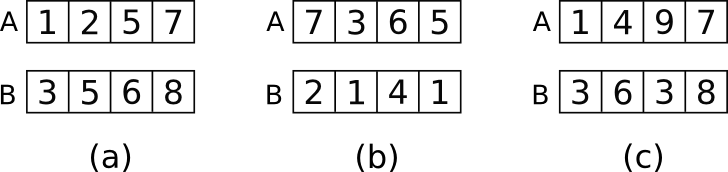
\includegraphics[width=100mm,natwidth=728,natheight=172]{bioinsp-dominance.png}
  \caption{Comparing solutions: (a) a is better than b, (b) b is better than a, (c) none is better - a and b are non-dominated}
  \label{fig:dominance}
\end{figure}

The Pareto Optimality theory defines the concept of Pareto Dominance, that can be used to compare two solutions. Figure \ref{fig:dominance2} gives an example of Pareto Dominance.

\begin{figure}[ht!]
  \centering
  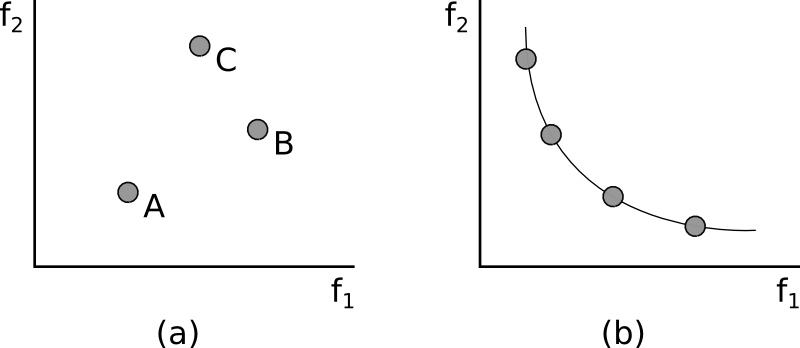
\includegraphics[width=110mm,natwidth=800,natheight=348]{bioinsp-dominance2.png}
  \caption{Pareto Dominance: (a) A dominates B and C, (b) all points are non-dominated}
  \label{fig:dominance2}
\end{figure}

\noindent\textbf{Definition (Pareto Dominance)}: a vector $\mathbf{u} = (u_1,...,u_k)$ is said to dominate a vector $\mathbf{v} = (v_1,...,v_k)$ (denoted by $\mathbf{u} \preceq \mathbf{v}$), if and only if $\mathbf{u}$ is partially less than $\mathbf{v}$, i.e., $\forall_i \in \{1,...,k\}, u_i \leq v_i \land \exists i \in \{1,...,k\}: u_i < v_i$.

In figure \ref{fig:dominance2}(a), we see that A dominates the solutions B and C, because
\begin{itemize}
  \item the values for $f_1$ and $f_2$ of A are the same or smaller than the corresponding values for B respectively C
  \item at least one of the values for A is smaller than the corresponding values for B respectively C
\end{itemize}
In figure \ref{fig:dominance2}(b) we see that no solution dominates another solution.

Using the concept of dominance, it is possible to define when a solution is optimal, this is known as Pareto Optimality.

\noindent\textbf{Definition (Pareto Optimality)}: a solution $\mathbf{x}$ is Pareto Optimal, if there is no $\mathbf{x'} \in \Omega$ for which $\mathbf{v} = \mathbf{F}(\mathbf{x'}) = (f_1(\mathbf{x'}),...,f_k(\mathbf{x'}))$ dominates $\mathbf{u} = \mathbf{F}(\mathbf{x}) = (f_1(\mathbf{x}),...,f_k(\mathbf{x}))$.

This means that no objective of a Pareto Optimal solution $\mathbf{x}$ can be improved without negatively affecting at least one of it's other objectives.

The solution to a MOP is then the set of non-dominated solutions, also called the Pareto Optimal Set.

\noindent\textbf{Definition (Pareto Optimal Set)}: for a given MOP $\mathbf{F}(\mathbf{x})$, the Pareto Optimal Set is defined as $\mathcal{P}^* = \{\mathbf{x} \in \Omega | \neg \exists \mathbf{x'} \in \Omega, \mathbf{F}(\mathbf{x'}) \preceq \mathbf{F}(\mathbf{x}) \}$

Its correspondence in the objective space (that is, the space where the results of the the objective functions lay) is called the Pareto Optimal Front, or just Pareto Front.

\noindent\textbf{Definition (Pareto Front)}: for a given MOP $\mathbf{F}(\mathbf{x})$ and Pareto Optimal Set $\mathcal{P}^*$, the Pareto Front $\mathcal{PF}^*$ is defined as $\mathcal{PF}^* = \{\mathbf{F}(\mathbf{x}) | \mathbf{x} \in \Omega \}$

When searching for the solutions of a MOP the goal is to find an approximation to the Pareto Front that:
\begin{itemize}
  \item has good convergence to the optimal Pareto Front, i.e. it is as near to the optimal Pareto Front as possible
  \item has good diversity, i.e. the solutions are well distributed throughout the Pareto Front
\end{itemize}

Figure \ref{fig:conv-div} gives an example for convergence and diversity of the Pareto Front. In figure \ref{fig:conv-div}(a) we have a Pareto Front with a bad convergence, as it is far away from the optimal/true Pareto Front. Figure \ref{fig:conv-div}(b) shows a Pareto Front that has bad divergence, i.e. several sections of the optimal Pareto Front are not covered with solutions. Figure \ref{fig:conv-div}(c) shows the ideal case, where the Pareto Front matches with the optimal Pareto Front - this is the desired solution.

\begin{figure}[ht!]
  \centering
  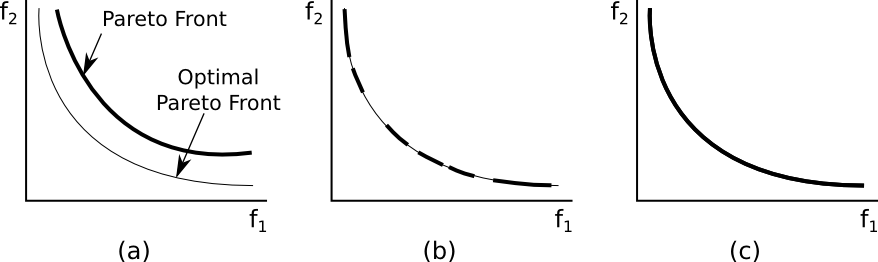
\includegraphics[width=130mm,natwidth=878,natheight=262]{bioinsp-conv-div.png}
  \caption{Example Pareto Fronts: (a) Pareto Front with bad convergence, (b) Pareto Front with bad divergence, (c) ideal case, where the Pareto Front matches the optimal Pareto Front}
  \label{fig:conv-div}
\end{figure}

\section{Complexity considerations}
Optimization is usually a computationally intensive task. For the TSP example, we can compute how many different solutions exist for a problem with $n$ cities, using formula \eqref{eq:tsp-cities}. Already a small number of cities entails a large number of solutions. For example, if we have 15 cities, we have a search space of over 43 billion solutions that we need to evaluate to get the best solution (assuming that we have no better suited technique to solve the problem). This number grows quickly if new cities are added and soon it becomes impossible to compute the optimal solution.

\begin{equation}\label{eq:tsp-cities}
  (n - 1)! / 2, \ \mbox{where} \ n \ \mbox{is the number of cities}
\end{equation}

Often there is no need to find the best solution to a problem, or there is no way at all. Instead it is sufficient to find a good enough solution in reasonable time. Approximation techniques can be used for this purpose. They don't guarantee to find the exact optimal solution, as they don't evaluate all solutions of the entire solution space. The advantage of approximation techniques is that they deliver solutions in a fast way. The results are usually near-optimal, although they can also be arbitrarily bad.

One well known family of approximation techniques are the metaheuristics \cite{yang2010nature}. A metaheuristic defines an abstract sequence of steps that leads to the optimization of a problem. As such, they are not problem specific and can be applied to a broad range of optimization problems.

\section{Optimization, inspired by nature}
Bio-inspired optimization techniques are a sub family of the metaheuristics. The name derives from the fact that they mimic behaviors observed in nature. For example, genetic algorithms (GA) \cite{sivanandam2008genetic} imitate the concept of evolution where only the fittest individuals survive and reproduce. Another example is particle swarm optimization (PSO) \cite{kennedy2010particle} that mimics the behavior of a flock of birds.

Bio-inspired optimization techniques are used today in many areas, like mechanical and electrical engineering, image processing, machine learning, network optimization, data mining etc. \cite{sivanandam2008genetic}.

\subsection{Genetic algorithm}
\label{chap:bioalgorithms:ga}
Genetic algorithms (GAs) are population-based optimization strategies. The population consists of $n$ individuals, each one representing a solution to the optimization problem. Every individual gets assigned a fitness value which represents its adoption to the environment. The fitness value is computed according to the optimization objective.

The idea behind genetic algorithms is to iteratively evolve the population towards individuals better adopted to the environment, which in an optimization problem means solutions of higher quality (preferably the optimum). The evolution is performed by applying selection, recombination and mutation to the population.

Recombination is performed by selecting two or more individuals out of the whole population. Those individuals are called the parent individuals. Fitter individuals are preferred for the recombination, as they have a high chance to produce fit offsprings. The parents are recombined using an operator called crossover. An example of a crossover operator is the computation of the mean value between the parents. The crossover results in one ore several child individuals. A mutation operator is then applied to the children, resulting in slightly mutated child individuals.

% Typically, in each iteration, a population of size $n$ generates $n$ child individuals, but there are also other strategies, e.g. a steady state reproduction strategy \cite{durillo2008study}.

At the end of each iteration, the fitness of all individuals (parents and children) is computed and the fittest individuals are selected to form the base population of the next iteration. This process is known as natural selection or survival of the fittest and leads intuitively towards fitter and better results. 

Algorithm \ref{algorithm:ga-pseudo} shows the pseudo code for a GA.

\begin{algorithm}
  \caption{Genetic algorithm}\label{algorithm:ga-pseudo}
  \begin{algorithmic}[1]
  \Procedure{GA}{}
  \State $\textit{P} \gets \text{generateInitialPopulation}$
  \State $\text{evaluate(} \textit{P} \text{)}$
  \While {$\text{!} \textit{terminationCriteria}$}
    \State $\textit{P'} \gets \text{recombine(} \textit{P} \text{)}$
    \State $\textit{P''} \gets \text{mutate(} \textit{P'} \text{)}$
    \State $\text{evaluate(} \textit{P''} \text{)}$
    \State $\textit{P} \gets \text{select(} \textit{P, P''} \text{)}$
  \EndWhile
  \Return best solution found so far
  \EndProcedure
  \end{algorithmic}
\end{algorithm}

The GA algorithm can be used to solve SOPs and MOPs. In the case of MOPs, the GA must be modified in order to produce a set of solutions that form a Pareto Front. A typical implementation of such a modification is NSGA-II \cite{deb2002fast}. In NSGA-II, the selection is performed based on ranking and crowding distance.

The ranks of the individuals are computed by iteratively finding the non-dominated solutions in the set of yet not ranked individuals, and assigning the current rank to them. The rank starts at 0, after each iteration, it increases by one. The iteration stops after all individuals are ranked.

The crowding distance is used to sort the best individuals of a given rank. This happens when $p$ out of $q$ individuals of a given rank need to be selected (with $q > p$). The crowding distance measures how distant neighboring solutions are to a given individual. Higher crowding distances are preferred, since this leads to better diversity in the final solution.

As an example, look at figure \ref{fig:rank-crowdingdist}. In figure \ref{fig:rank-crowdingdist}(a) we have a population of three individuals, namely A, B and C. As one can see from the figure, A is non-dominated, but dominates B and C. So, if we want to apply the ranking algorithm, rank 0 is assigned to A (because A is non-dominated). Then, the rank is increased by one. Now we have two individuals that are yet not ranked, B and C. Those individuals are again non-dominated, because we don't consider A anymore, which is already ranked. The rank of 1 is applied to A and B. After this iteration, the ranking algorithm stops, because all individuals have a rank.

Figure \ref{fig:rank-crowdingdist}(b) gives a graphical representation of crowding distance that is used to select the $p$ out of $q$ best solutions for individuals with the same rank.

\begin{figure}[ht!]
  \centering
  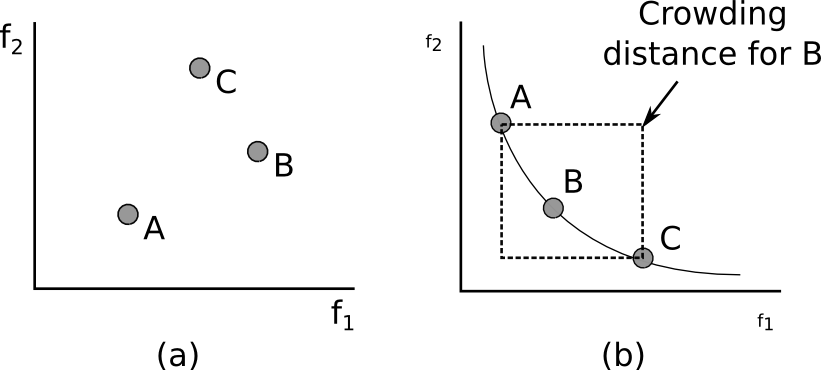
\includegraphics[width=110mm,natwidth=821,natheight=370]{bioinsp-rank-crowdingdist.png}
  \caption{Ranking and crowding distance: (a) A has rank 0, B and C rank 1, (b) crowding distance of solution B}
  \label{fig:rank-crowdingdist}
\end{figure}

\subsection{Particle swarm optimization}
The particle swarm optimization algorithm (PSO) mimics the behavior of a flock of birds. The birds in a flock usually follow a highlighted bird, for example the first one. If the highlighted bird changes its direction, the other birds will also adjust their direction. This principle can be used for optimization.

In PSO, the population consists of a number of particles (birds). Each particle has a position, a velocity and a fitness value. Each particle knows about the global best solution found so far (gBest), and its personal best solution (pBest), found so far. A particle moves in the direction of gBest and pBest. For this, in each iteration the particle adjusts its velocity according to its current velocity and the distance to gBest and pBest. Then it moves according to the adjusted velocity. This simple behavior lets the particle converge towards gBest.

The PSO can be implemented using a simple vector operation, given in formula \eqref{eq:pso-speed}.

\begin{equation}\label{eq:pso-speed}
  v(t) = w * v(t - 1) + c_1 * r_1 * (pBest - x(t - 1)) + c_2 * r_2 * (gBest - x(t - 1))
\end{equation}

This vector operation is performed for each iteration on all particles. $v(t)$ is the velocity of the particle at time $t$, $v(t - 1)$ is the velocity in the previous iteration and $x(t - 1)$ defines the position of the particle, also in the previous iteration. $w$ is called the inertia weight and defines the influence of the current speed on the new velocity. The parameter $c_1$ is called the cognitive acceleration coefficient and defines how much the particle is influenced by its personal best solution. $c_2$ is called the social acceleration coefficient and defines how much the particle is influenced by the global best solution. The parameters $r_1$ and $r_2$ are random values between 0 and 1 and are used as a source of diversity.

After the particles velocity is computed, its current position is updated using formula \eqref{eq:pso-position}
\begin{equation}\label{eq:pso-position}
  x(t) = v(t) + x(t - 1)
\end{equation}

\begin{figure}[ht!]
  \centering
  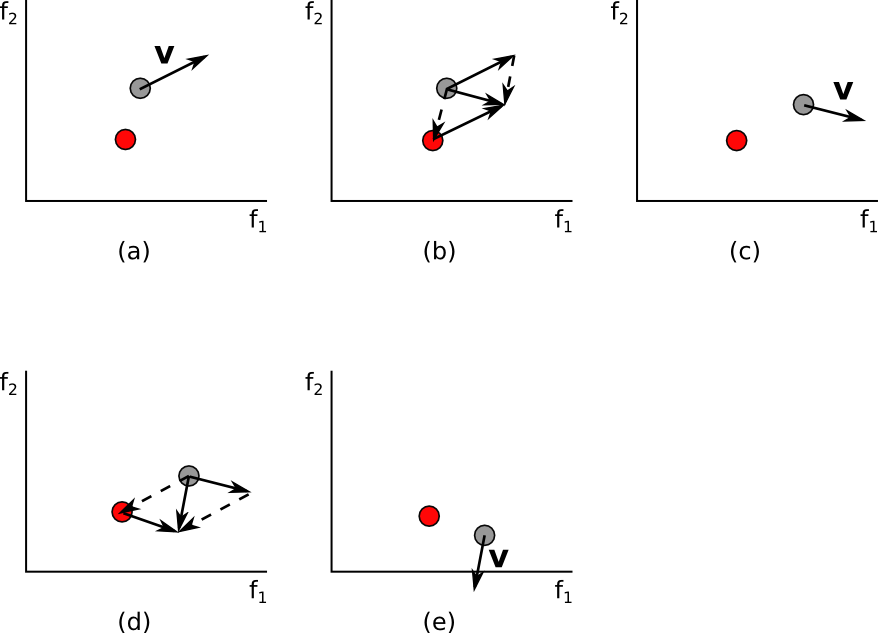
\includegraphics[width=130mm,natwidth=929,natheight=1037]{bioinsp-pso.png}
  \caption{Four iterations of PSO for a single particle. The red dot marks gBest, the gray dot the particle. The velocity and position of the particle does rely only on gBest in this example, pBest is not used}
  \label{fig:pso}
\end{figure}

An example of four iterations for a single particle can be found in figure \ref{fig:pso}. Figure \ref{fig:pso}(a) shows the initial situation, the red dot highlights gBest, the gray dot the particle. Figure \ref{fig:pso}(b) shows how the current velocity and position of the particle, as well as the position of gBest, influence the velocity and position of the particle in the next iteration, which is shown in figure \ref{fig:pso}(c). Figure \ref{fig:pso}(d) to \ref{fig:pso}(i) show additional iterations, all conforming to the same principle. The value of pBest is not considered in this example.

PSO can also be used to compute solutions to a MOP. In this case, the non-dominated solutions are stored in an archive. New solutions are inserted into the archive if they are non-dominated by the elements in the archive. Subsequently the archive is scanned for dominated solutions that can arise from new inserted solutions. The dominated solutions are removed from the archive. The non-dominated solutions to the MOP can be extracted from the archive after PSO terminates.

\section{Parallelization using the island model}
\label{chap:bioalgorithms:island-model}
The island model is a high level parallelization model that is sometimes used in optimization problems. In the island model, several optimization algorithms run in parallel, trying to compute the result to the same problem. The parallel running algorithms are called the islands. Each of these algorithms is independent of the others, and each one may have a different solution at a given point of time. By exchanging their data after some intervals, islands may get interesting solutions from other islands that can be integrated in their own computation to enhance their solution. If we take the GA as an example, the islands would consist of independently running GAs that exchange individuals to improve the solution. Figure \ref{fig:island-model} shows an example island model with 3 GAs that exchange individuals.

\begin{figure}[ht!]
  \centering
  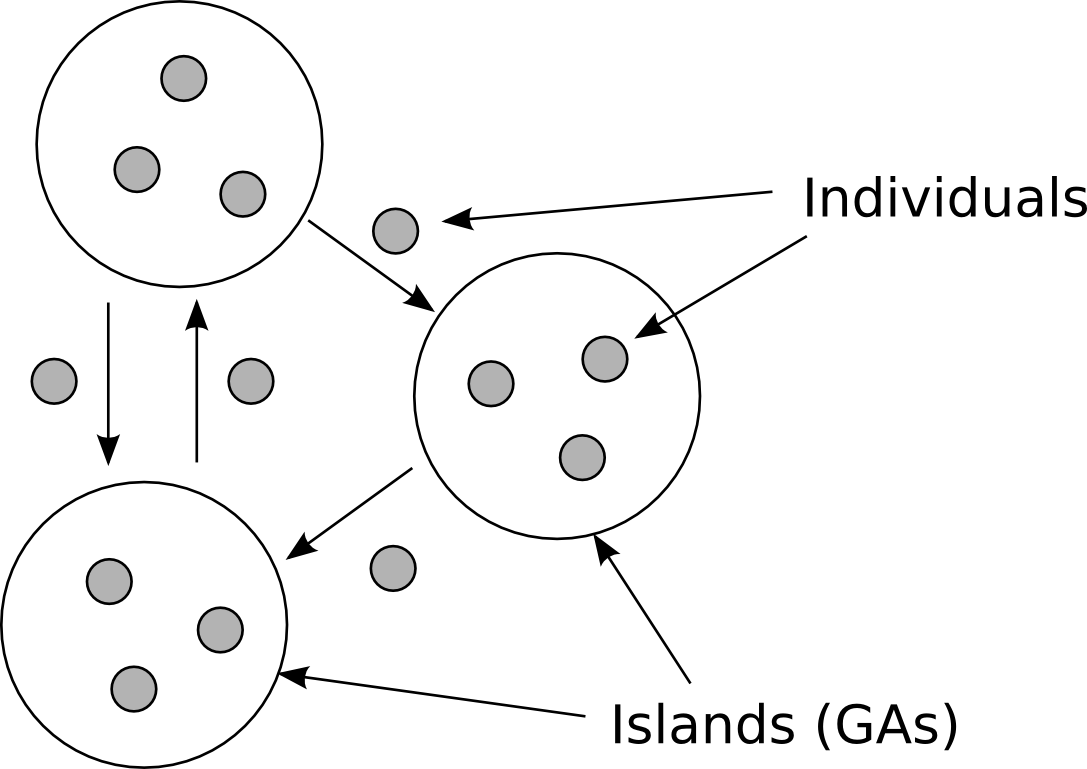
\includegraphics[width=70mm,natwidth=1087,natheight=769]{island-model.png}
  \caption{Example island model with 3 GAs, exchanging individuals}
  \label{fig:island-model}
\end{figure}

The island model enhances the exploratory behavior of optimization algorithms, which often results in better overall solutions. As the data exchange is only done at certain points of time, the islands have the chance to exploit their own solution. When they get stuck in a local optima, they get the chance to escape this optima by considering solutions from other islands.

Biohadoop, the framework implemented during this thesis, provides the capabilities to execute an island model. More information can be found in \ref{chap:impl:island-model}.

% \subsection{Ant colony optimization}
% The ant colony optimization (ACO) is an optimization technique for combinatorial problems, like the TSP. It is inspired by ant colonies, that are very effective in finding shortest paths from their nest to a source of food.
% 
% To find this paths, ants deposit a pheromone on the track they are using. The pheromone evaporates over time, such that paths that are frequently used (for example because they are shorter), have more pheromones applied, than seldom used paths. If an ant must decide which path to take, it follows with a higher probability the path that has the most pheromones applied. While using this path, it applies again pheromones, which increases the probability that other ants will follow this path.
% 
% Individually, the ants take only simple decisions, based on the amount of pheromones on a given path. Collectively, they work on solving an optimization problem.
% \chapter{Hadoop}
\label{chap:hadoop}
Apache Hadoop is an open source software project for massive data processing and parallel computing in a cluster. It derives from Google's publications about MapReduce \cite{dean2008mapreduce} and Google File System (GFS) \cite{ghemawat2003google}, but has undergone quite some changes due to its active development, e.g., the introduction of YARN (see section \ref{chap:hadoop:yarn}).

Hadoop is designed to run on commodity hardware and provides a high degree of fault tolerance, implemented in software. It scales from a single server up to thousands of machines. Each machine stores data and is used for computation.

In the following key properties of Hadoop are listed:
\begin{description}
  \item[Scalability]: Hadoop is able to scale horizontally, which means that the performance scales with the number of cluster machines. The performance can be improved by dynamically adding nodes at runtime if required. Furthermore, unnecessary nodes can be shut down if their additional performance is not needed.
  \item[Cost effectiveness]: Since Hadoop runs on commodity hardware there is no need for exclusive, specialized proprietary hardware. It is possible to run Hadoop on an existing infrastructure. Hadoop runs also in the cloud. Different offers from Amazon, Google, Cloudera, etc. exist. This can further reduce costs, as the customer has to pay only for the resources used and doesn't need to maintain its own data center.
  \item[Flexibility]: Hadoop can handle any kind of data. Custom applications running on Hadoop enable the transformation of, and computation on arbitrary data. For example, Hadoop can be used to analyze log files. It can equally well be used by physicists to find patterns in their huge datasets.
  \item[Fault tolerance]: Hadoop expects hardware failures and is designed from ground up with fault tolerance in mind. If a machine fails, Hadoop automatically redirects the computations and data of this machine to another machine.
\end{description}

Hadoop consists of two main components, HDFS (Hadoop Distributed File System) and YARN (Yet Another Resource Manager). HDFS is a distributed, scalable and reliable file system. YARN assigns resources (CPU, memory, and storage) to applications running on a Hadoop cluster and is part of Hadoop since version 2.0. It replaced the resource management capabilities, that were bundled in MapReduce prior to Hadoop version 2.0. Since this version, MapReduce uses YARN for the resource management.

YARNs concept of resources is more flexible than the MapReduce resource management model used for Hadoop prior to version 2.0. The old resource management is tailored to MapReduce tasks and divides the cluster resources into separate map and reduce slots. Map tasks and reduce tasks are only executed on map slots and reduce slots, respectively. The number of map and reduce slots are statically configured and established during the startup of Hadoop. This can lead to poor resource usage if the MapReduce applications don't fit to the configured number of slots. The situation gets even worse for applications with a different computational model like Biohadoop, which provides a framework for iterative computations. With the old resource management model iterative tasks run either on the map slots or on the reduce slots while unused slots idle. Therefore, resources are not fully exploited. YARN, on the other hand, is able to host arbitrary computational models, as it provides the resources in an application agnostic way. More details about YARNs resource management can be found in section \ref{chap:hadoop:yarn}.

Figure \ref{fig:hadoop-layer} shows the current architecture of Hadoop. HDFS provides data services as the basic layer. YARN builds on top of HDFS and manages the resources of the cluster. The different applications, like MapReduce, Storm, Spark, Biohadoop, etc. run on top of YARN.

\begin{figure}
  \centering
  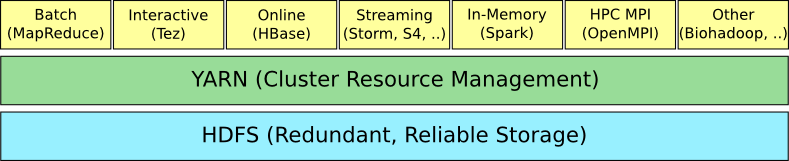
\includegraphics[width=130mm,natwidth=789,natheight=161]{hadoop-layer.png}
  \caption[Hadoop layers]{Hadoop layers: HDFS forms the base and provides data services, YARN builds on it and provides resource management. The applications run on top of YARN.}
  \label{fig:hadoop-layer}
\end{figure}

\section{HDFS}
\label{chap:hadoop:hdfs}
HDFS is the distributed, scalable and reliable file system of Hadoop, written in Java. A HDFS cluster consists of a single NameNode and several DataNodes. The NameNode manages the file system namespace, regulates the client access to files, commands the DataNodes and decides where to store the data. A DataNode stores the assigned data on the storage that is attached to its cluster node (usually there is one DataNode running on each cluster node). HDFS performs file transfer and storage only between clients and DataNodes or among DataNodes. The NameNode never comes directly in touch with the user data. This way, HDFS can scale by adding more DataNodes.

The files in HDFS are stored in blocks of a configurable maximum size (default 128MB). Reliability arises from the replication of blocks to other available DataNodes. The decision where to store data replicas is made by the NameNode, the exchange of replicas is performed directly between the DataNodes. The number of replicas is configurable and has a default value of 3, which means that each block is stored three times in HDFS. If a node goes down, for example because of a hardware failure, HDFS automatically replicates this node's data blocks to other nodes by using the remaining copies, such that the replication factor is satisfied again. Files that are bigger than the maximum block size are split into several smaller blocks. The resulting blocks are handled as described above.

The restriction of a single NameNode instance makes the NameNode effectively a single point of failure, but there exist solutions for high availability that make use of a Quorum Journal manager \footnote{\url{http://hadoop.apache.org/docs/current/hadoop-project-dist/hadoop-hdfs/HDFSHighAvailabilityWithQJM.html} last access: 12.11.2014} or NFS.\footnote{\url{http://hadoop.apache.org/docs/current/hadoop-project-dist/hadoop-hdfs/HDFSHighAvailabilityWithNFS.html} last access: 12.11.2014}

Figure \ref{fig:hadoop-hdfs} shows how HDFS organizes the data. Here, each file is replicated twice (replication factor of 2). Note how HDFS tries to store block replicas on different nodes. For the sake of simplicity, all files in this example are smaller than the HDFS maximum block size, thus fitting in a single block.

\begin{figure}
  \centering
  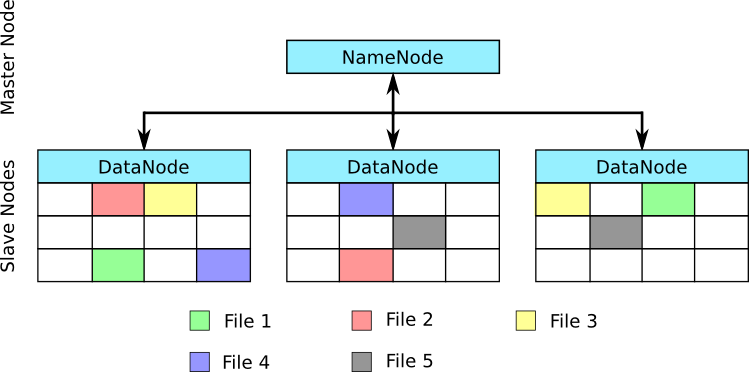
\includegraphics[width=130mm,natwidth=749,natheight=372]{hadoop-hdfs.png}
  \caption[HDFS file storage]{HDFS file storage, each file is replicated twice.}
  \label{fig:hadoop-hdfs}
\end{figure}

HDFS provides rack awareness, which allows applications to consider the physical location of a machine when data has to be stored or moved. Rack awareness allows for a variety of advanced features, e.g., it is faster to execute computations on the nodes where the required data is already available instead of first moving the data to another node. This minimizes possibly slow data traffic. Another example is HDFS itself, that uses its rack awareness for its performant replication process, while considering the physical location of the replicas.

\section{YARN}
\label{chap:hadoop:yarn}
YARN is the resource manager of Hadoop. It schedules and satisfies resource requests of applications. It also monitors running applications. Resources are granted in form of resource containers, that consist of CPU, RAM, storage etc.

The functionality of YARN is provided by one ResourceManager and several NodeManagers (similar to HDFS). This architecture offers the needed scalability. Like in HDFS, the ResourceManager is a single point of failure, but solutions for high availability do also exist here in the form of standby ResourceManagers.\footnote{\url{http://hadoop.apache.org/docs/current/hadoop-yarn/hadoop-yarn-site/ResourceManagerHA.html} last access: 13.11.2014}

The ResourceManager has two components, the Scheduler and the ApplicationsManager. The Scheduler allocates resources for running applications but performs no monitoring of running applications. This is the job of the ApplicationsManager. The ApplicationsManager is responsible for accepting new application submissions, negotiating the first container of an application and monitoring of running applications. The monitoring aspect allows the ApplicationsManager to automatically restart failed applications.

The NodeManager (usually one per node) is responsible for the containers, that run on its node. It monitors their resource usage and reports this information back to the ResourceManager.

A typical YARN application consists of three components:

\begin{description}
  \item[Client]: this is the starting point of every YARN application. It submits the application to the ResourceManager, which allocates a free container in the cluster and starts the ApplicationMaster inside this container.
  \item[ApplicationMaster]: the ApplicationMaster (not to confuse with the ApplicationsManager) communicates with the ResourceManager. The ApplicationMaster can request additional containers, for example if it wants to distribute some of its work. It can return already allocated containers, if they are not needed. And it provides information about its current status via a heartbeat. The heartbeat is used by the ApplicationsManager to determine if the application is still alive or needs to be restarted.
  \item[Additional Containers]: the additional containers are not mandatory, but can be useful, as they provide additional resources. The containers can be used to offload work to them, for example in a master-worker scheme, like implemented in Biohadoop. The master runs on the ApplicationMaster and starts several containers. Each container runs a worker.
\end{description}

There is no defined way for data exchange between an ApplicationMaster and its additional containers. If data exchange is a requirement, it must be implemented separately. To see how this is done in Biohadoop, confer to section \ref{chap:impl:communication}.

The automatic restart capabilities of YARN are not extended to additional containers, as there is no general valid solution for their restart. For example, some containers need to maintain state, which must be reflected on a restart. Other containers may work in a stateless fashion. What YARN does, is to provide information about the states of its additional containers to the ApplicationMaster. This way, the ApplicationMaster can implement the restart of failed containers on its own.

YARN runs applications simultaneously, as long as there are enough cluster resources available. Applications are queued if the currently available resources are not sufficient. Figure \ref{fig:hadoop-app} shows an example for the occupation of a Hadoop cluster with one master node and three slave nodes. The NameNode (HDFS) and ResourceManager (YARN) run on the master node, the DataNodes (HDFS) and NodeManagers (YARN) run on the slave nodes and communicate with the corresponding services on the master node. The applications are started by the clients, that request an initial container for their ApplicationMaster from the ResourceManager. After the ApplicationMasters are started they in turn request additional containers from the ResourceManager. In this example, two applications are started. Application 1 occupies five containers and Application 2 occupies seven containers.

\begin{figure}
  \centering
  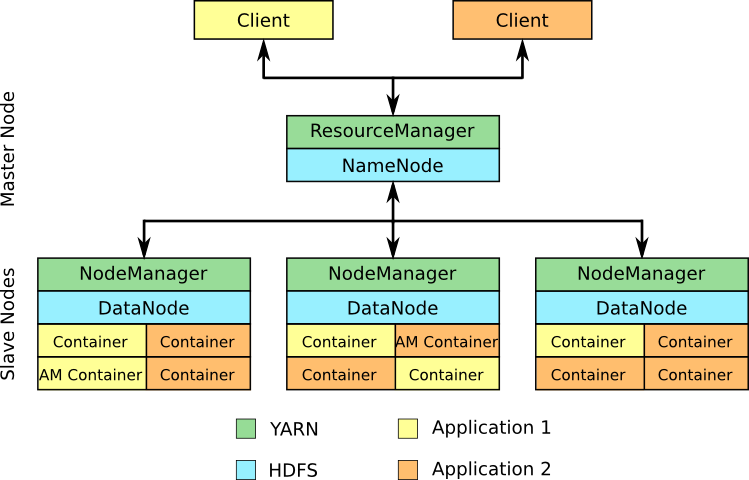
\includegraphics[width=130mm,natwidth=749,natheight=480]{hadoop-app.png}
  \caption[Occupation of a Hadoop cluster for two applications]{Occupation of a Hadoop cluster for two applications. The NameNode (HDFS) and ResourceManager (YARN) run on the master node. DataNodes (HDFS) and NodeManagers (YARN) run on the slave nodes and communicate with the corresponding services on the master node. The applications, including the ApplicationMasters (AM container), run on the slave nodes inside containers.}
  \label{fig:hadoop-app}
\end{figure}

\section{Oozie}
\label{chap:hadoop:oozie}
Apache Oozie is a workflow tool, that runs on Hadoop. The workflow jobs are Directed Acyclic Graphs (DAGs) of actions, written in XML.\footnote{\url{http://www.w3.org/TR/xml/} last access: 09.01.2015} Oozie uses an internal scheduler to make decisions about the submitted workflows and their progress, the action execution is delegated to Hadoop.

Each Oozie action has two possible outcomes: ``ok'' if the action completed successfully, and ``error'' in the case of an error. The action outcome influences the next transition in the DAG. 

An Oozie workflow consists of two types of nodes, the control flow nodes and the action nodes. Control flow nodes define the sequence of actions in a workflow (start, end, failure, decision, fork, join). Action nodes are used to execute a program or computation.

Oozie provides a number of default actions, like the Java action, that can be used to start a YARN application. Other actions include MapReduce actions, HDFS file system actions (move, delete and mkdir), Email, etc. Oozie allows also to implement new custom actions, that expose different behaviors. In the course of this work a custom action was implemented to invoke Biohadoop from Oozie. More details about this custom action and its configuration can be found in chapter \ref{chap:impl:oozie}.

Figure \ref{fig:oozie-example} shows a workflow example. It is started at the control flow node labeled ``Start'' followed by  the ``FS action''. The transition to the next step is depending on the result of this action. Actions ``Failed'' and ``Fork'' are invoked in case of an error or success, respectively. The ``Fork'' action starts two Java actions in parallel. Actions performed inside a ``Fork'' action have a special error semantic. If an error occurs in any of the parallel actions inside a fork node, all parallel actions are considered as failed. If no error happened, the ``Join'' node waits for two (or possibly more) parallel actions to finish. Then, a ``Decision'' action is invoked, that transitions to the ``MapReduce'' action if the needed conditions are given. If the whole workflow has no errors it terminates at the ``End'' node.

\begin{figure}
  \centering
  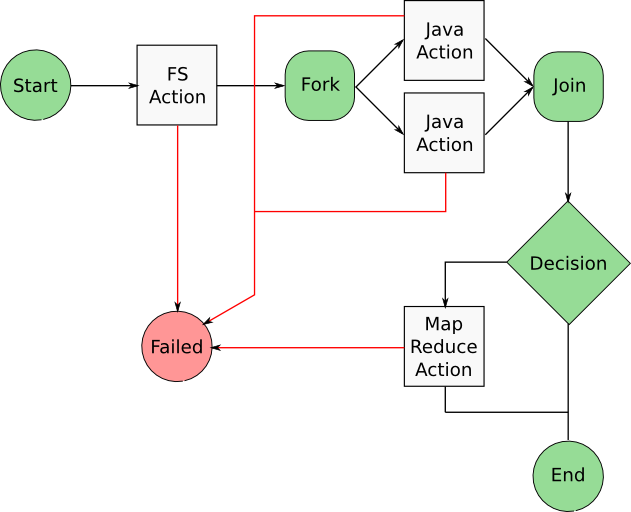
\includegraphics[width=100mm,natwidth=631,natheight=512]{oozie-example.png}
  \caption[Oozie workflow transitions]{Oozie workflow transitions. If any action returns with an error, the workflow transitions to the final state ``Failed'', else the workflow advances according to the defined sequence.}
  \label{fig:oozie-example}
\end{figure}

It can be difficult and error prone to manually write a workflow XML. Graphical tools like Hue \footnote{\url{http://gethue.com/category/oozie/} last access: 26.12.2014} can simplify this process.
\chapter{Implementation}
\label{chap:impl}

\section{System architecture}
\label{chap:impl:system-architecture}
Biohadoop is a framework to parallelize algorithms on Apache Hadoop. It works according to the master - worker principle, where one master commands several workers. The master runs an algorithm whose compute intensive parts are executed by the workers in parallel. Time consuming sections of an algorithm, that can be parallelized, are good candidates to run on the workers.

The genetic algorithm (GA) from chapter \ref{chap:bioalgorithms:ga} is used in the following sections as an example of how to parallelize an algorithm for the master - worker scheme. A GA is an iterative procedure, each iteration creates a set of new individuals (offsprings), evaluates their fitness and selects the best individuals for the next iteration, based on the fitness of all GA individuals. The creation of an offspring and its subsequent fitness evaluation can be combined into a single function. This function consumes most of the time in a GA, but it can be executed in parallel, as it depends only on its input values (the parents) and has no side effects. It is therefore a good example of a parallel task that can be performed by workers, while the rest of the GA algorithm runs on the master (see figure \ref{fig:master-worker}).

\begin{figure}[ht!]
  \centering
  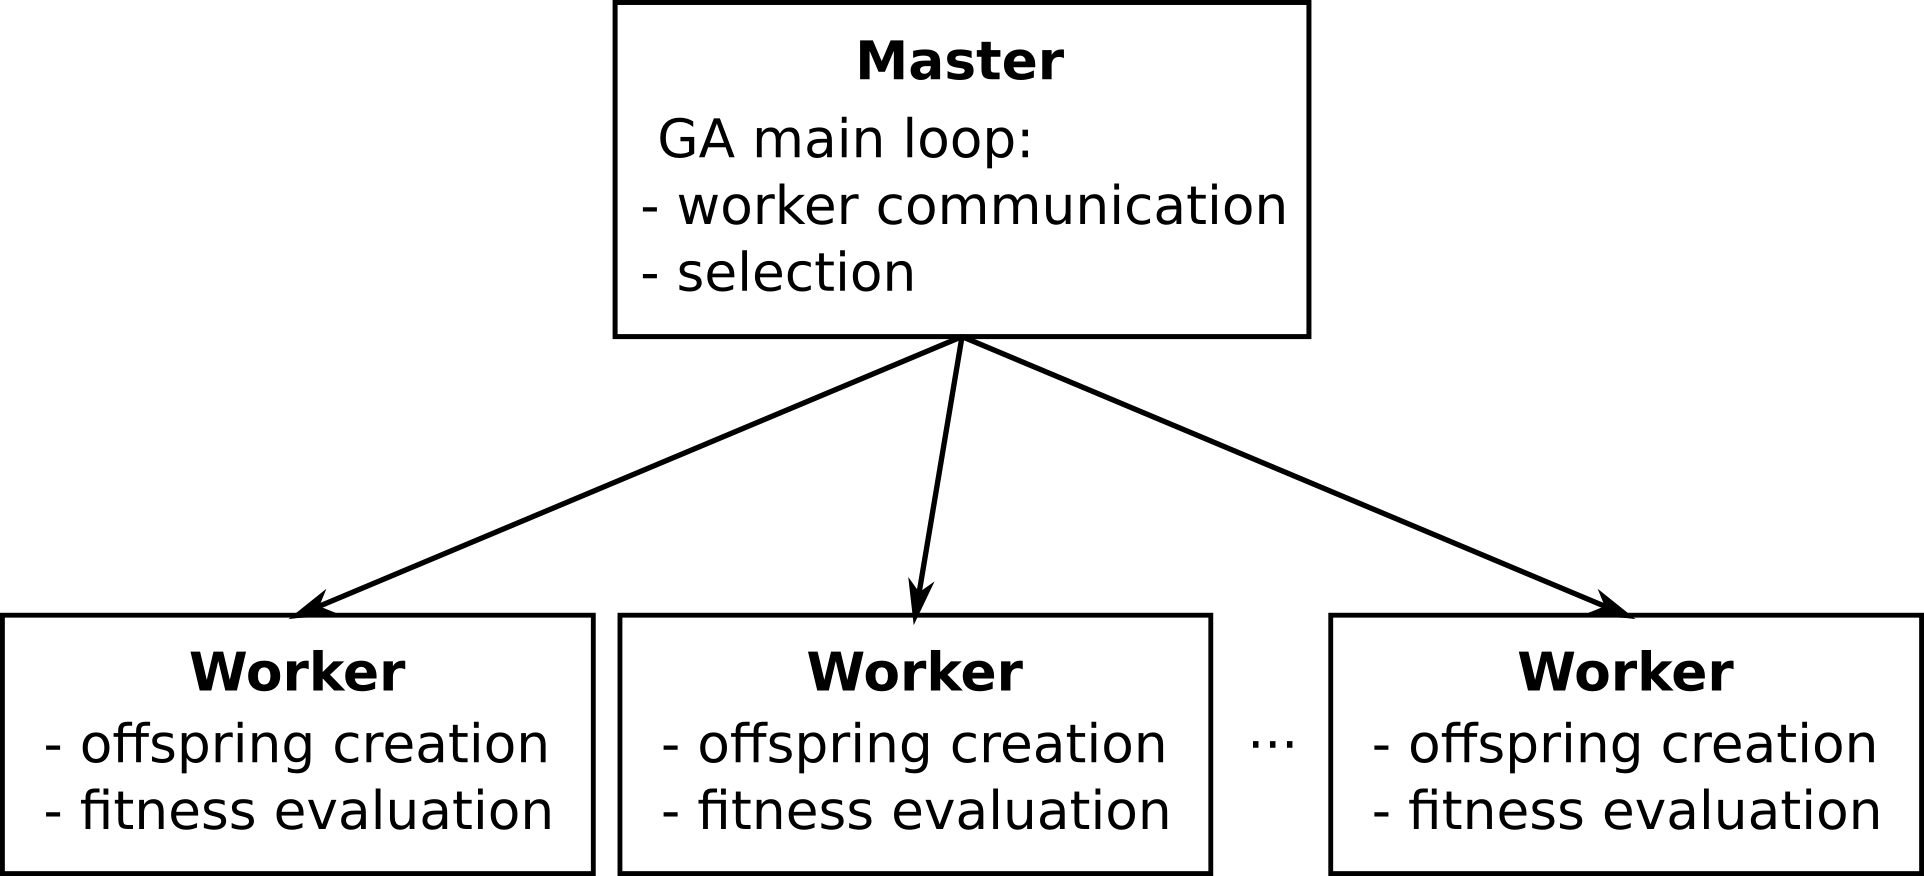
\includegraphics[width=100mm]{master-worker.png}
  \caption{Master - worker principle for a GA, one master commands several workers. The master runs the main loop, where it communicates with the workers to get new individuals. Then it selects the best individuals to become the population of the next iteration.}
  \label{fig:master-worker}
\end{figure}

The master - worker architecture was chosen for Biohadoop, because many algorithms can be parallelized by this approach, like the GA and the PSO presented in chapter \ref{chap:bioalgorithms}. Another reason is that the master - worker scheme maps very well to YARN (see chapter \ref{chap:hadoop:yarn}).

Biohadoop is written to run as a YARN application and provides features, that otherwise need to be implemented manually, such as:

\begin{itemize}
  \item support for the execution of several algorithms at the same time in a single Biohadoop instance. This has the advantage that workers, and therefore resources, can be shared by the algorithms. It guarantees also that the algorithms run at the same time. This guarantee can't be given when several Biohadoop instances are used, as YARN decides when it executes a scheduled application
  \item asynchronous communication between master and workers using the task system (section \ref{chap:impl:task-system}). YARN doesn't provide a default communication facility between its containers
  \item storage and load of arbitrary data sets to and from a file system (section \ref{chap:impl:persistence})
  \item support for the island model, a high level parallelization that can be used to improve the optimization performance of bio-inspired optimization techniques by exchanging results between multiple instances of an algorithm (section \ref{chap:impl:island-model})
  \item support for Apache Oozie through a custom action (section \ref{chap:impl:oozie}). This custom action can be used to schedule one or many Biohadoop instances. It also allows the usage of Biohadoop in a larger workflow
\end{itemize}

Every YARN application needs a client that submits the application to YARN. The YARN client in Biohadoop is implemented in the class \texttt{BiohadoopClient}. It is the main entrance point to run Biohadoop in a Hadoop environment and responsible to start the ApplicationMaster under the control of Hadoop.

Biohadoops ApplicationMaster starts the configured workers using additional YARN containers, and as it is the master in the master - worker scheme, it executes the configured algorithms and communicates with the workers. The ApplicationMasters main class is \texttt{BiohadoopApplicationMaster}. In a local (development) environment, it acts as the main entrance point to run Biohadoop without YARN (more on how to run Biohadoop can be found in \ref{chap:usage:run}).

The workers are started in additional YARN containers, each worker resides in a dedicated container.

Figure \ref{fig:architecture} shows how Biohadoops architecture maps to the architecture of a typical YARN application. It also gives a first impression of the task system that hides the technical details of the master - worker scheme from the algorithm. The task system consists of a task broker, one ore more endpoints and one or more workers.

\begin{figure}[ht!]
  \centering
  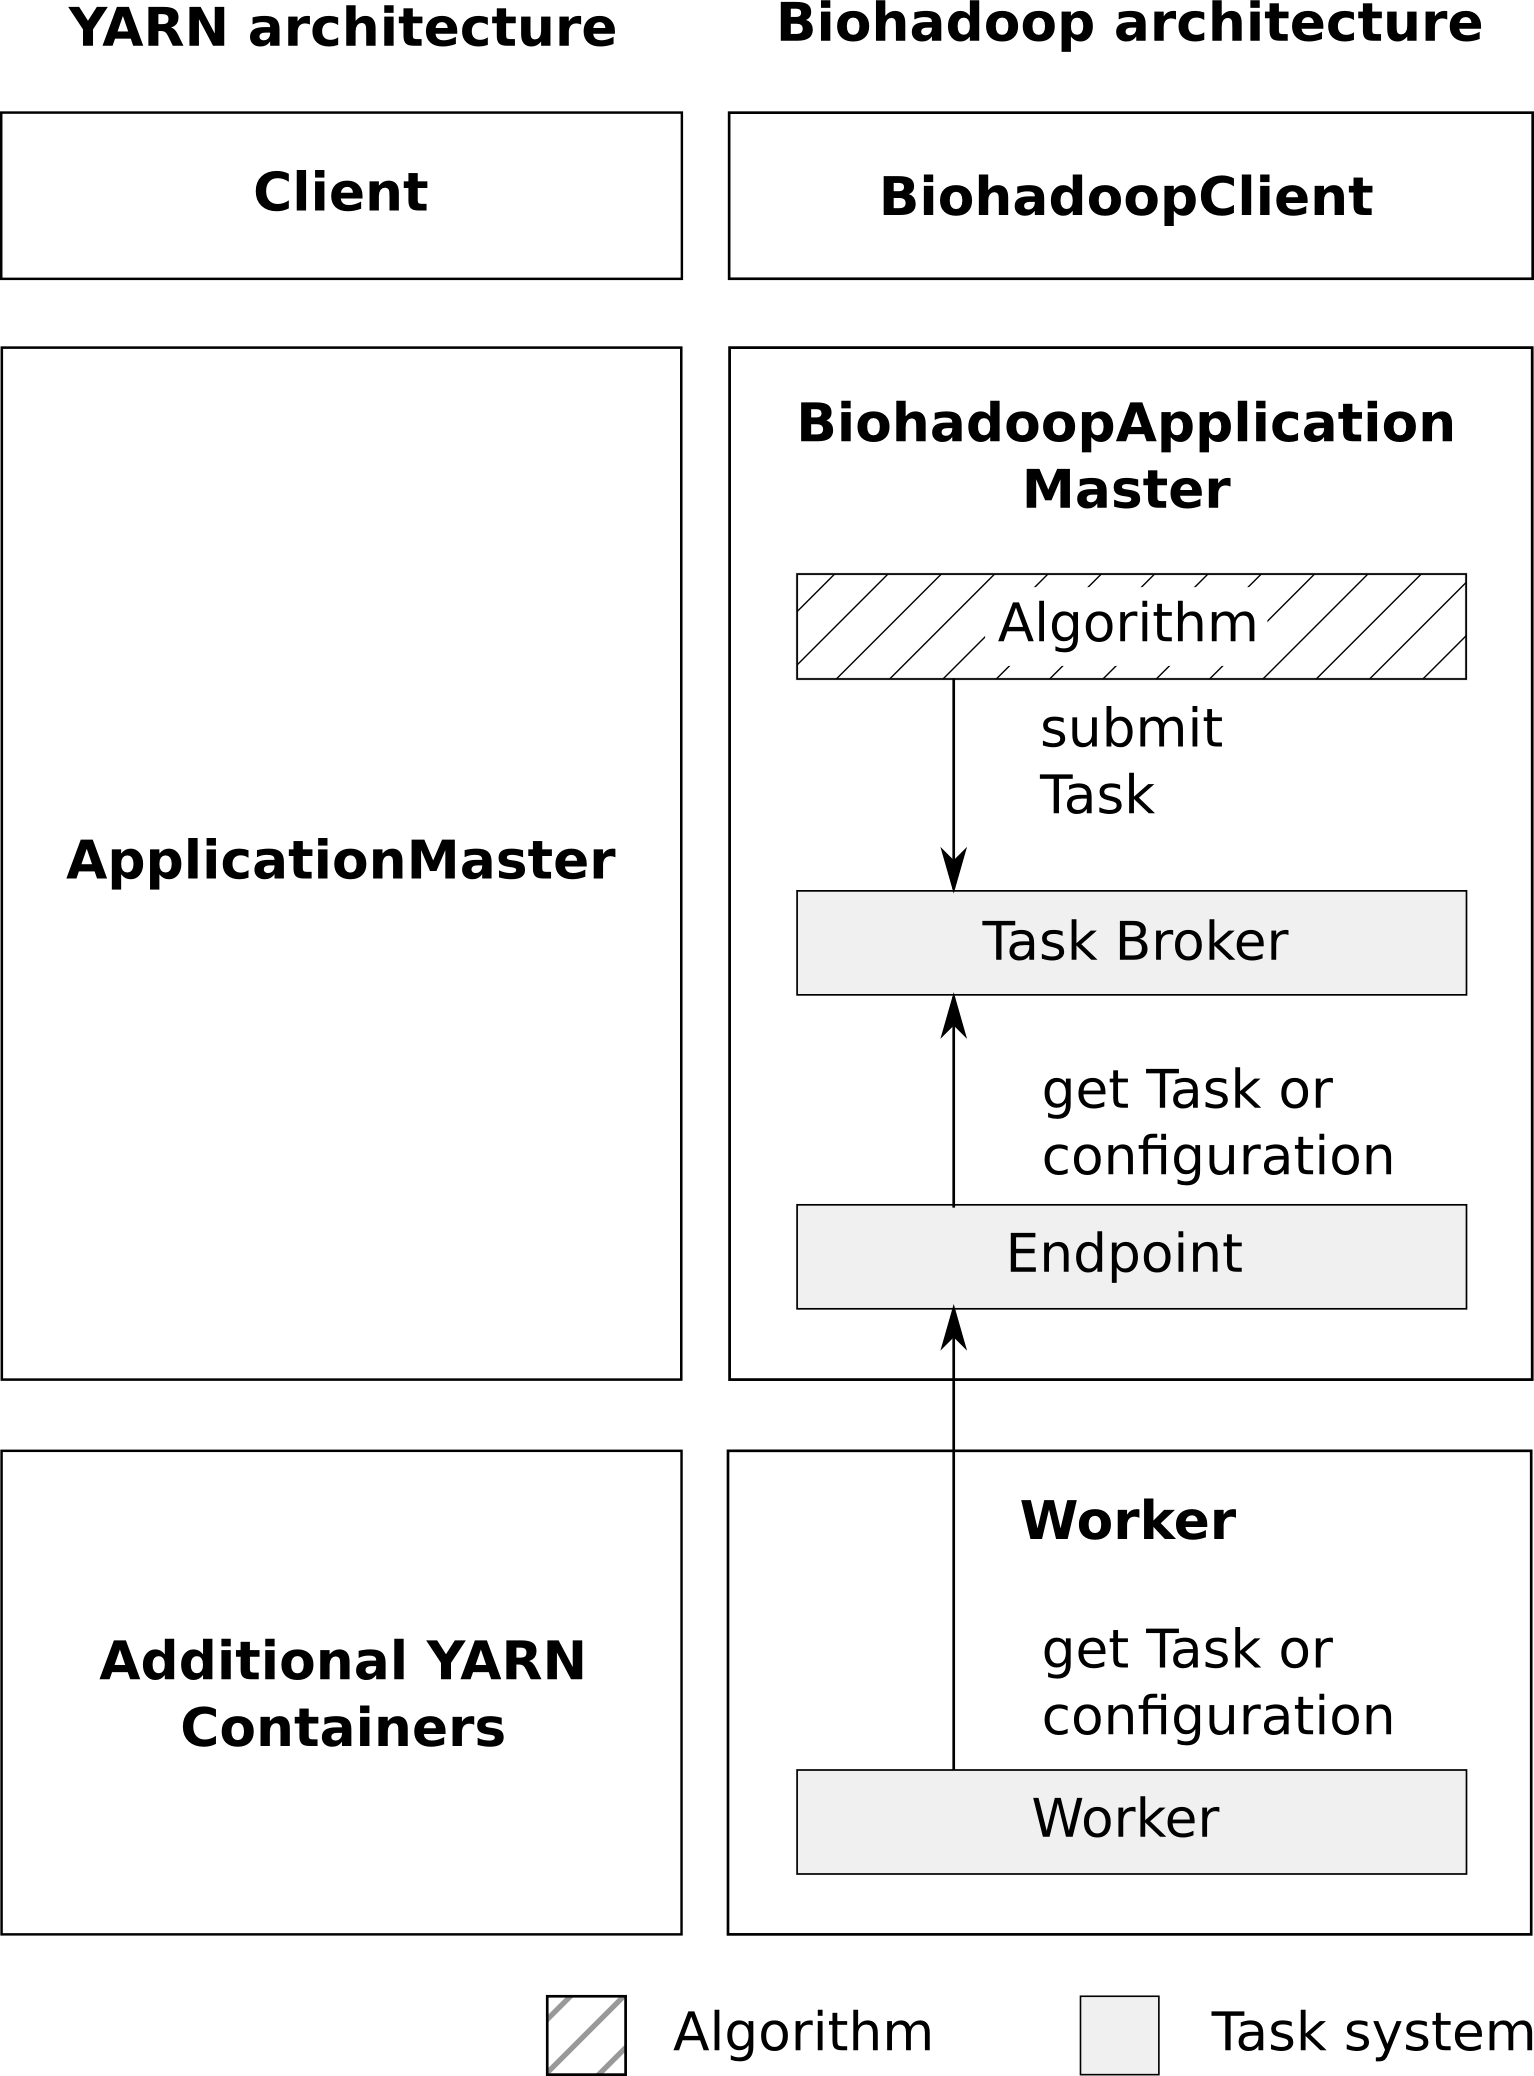
\includegraphics[width=80mm]{architecture.png}
  \caption{The figure shows, how the Biohadoop architecture maps to the architecture of a typical YARN application}
  \label{fig:architecture}
\end{figure}

An algorithm uses the task system to submit work items, from here on called tasks, to the workers and wait for the results. A task contains data and a reference to a task configuration that defines how to compute the result for the task. In the GA example, a task would be to create individuals and compute their fitness. In this case, the task data represents the parent individuals that are used to create an offspring. The configuration defines the method for offspring creation and fitness computation.

Submitted tasks are queued by the task broker. Endpoints get tasks from the broker and send them to waiting workers. The workers execute the configured computations on the tasks and return the results to the endpoints, that promote the results back to the broker and from there to the algorithms.

A task configuration is usually shared by many tasks, for example each task in the GA uses the same method to compute an offspring and its fitness value. Therefore, a task configuration is send to a worker only the first time it is needed, and cached by the worker otherwise. This reduces the communication amount between the master and the workers.

Figure \ref{fig:task-conf-reuse} shows how a worker requests tasks or task configurations to compute the result for a task. The worker requests a task from the master in picture \ref{fig:task-conf-reuse}(a), which is delivered in \ref{fig:task-conf-reuse}(b). The worker then recognizes that it doesn't know how to compute the result for the task - it has to request the task configuration in \ref{fig:task-conf-reuse}(c). The task configuration is returned in \ref{fig:task-conf-reuse}(d), the worker can now compute the task result in \ref{fig:task-conf-reuse}(e). The result is returned in \ref{fig:task-conf-reuse}(f), together with the request for the next task. The next task is delivered in \ref{fig:task-conf-reuse}(g) and as it uses the same task configuration as the prior task, the worker can reuse this configuration and directly compute the result in \ref{fig:task-conf-reuse}(h), after which the result is returned together with the request for the next task.

\begin{figure}[ht!]
  \centering
  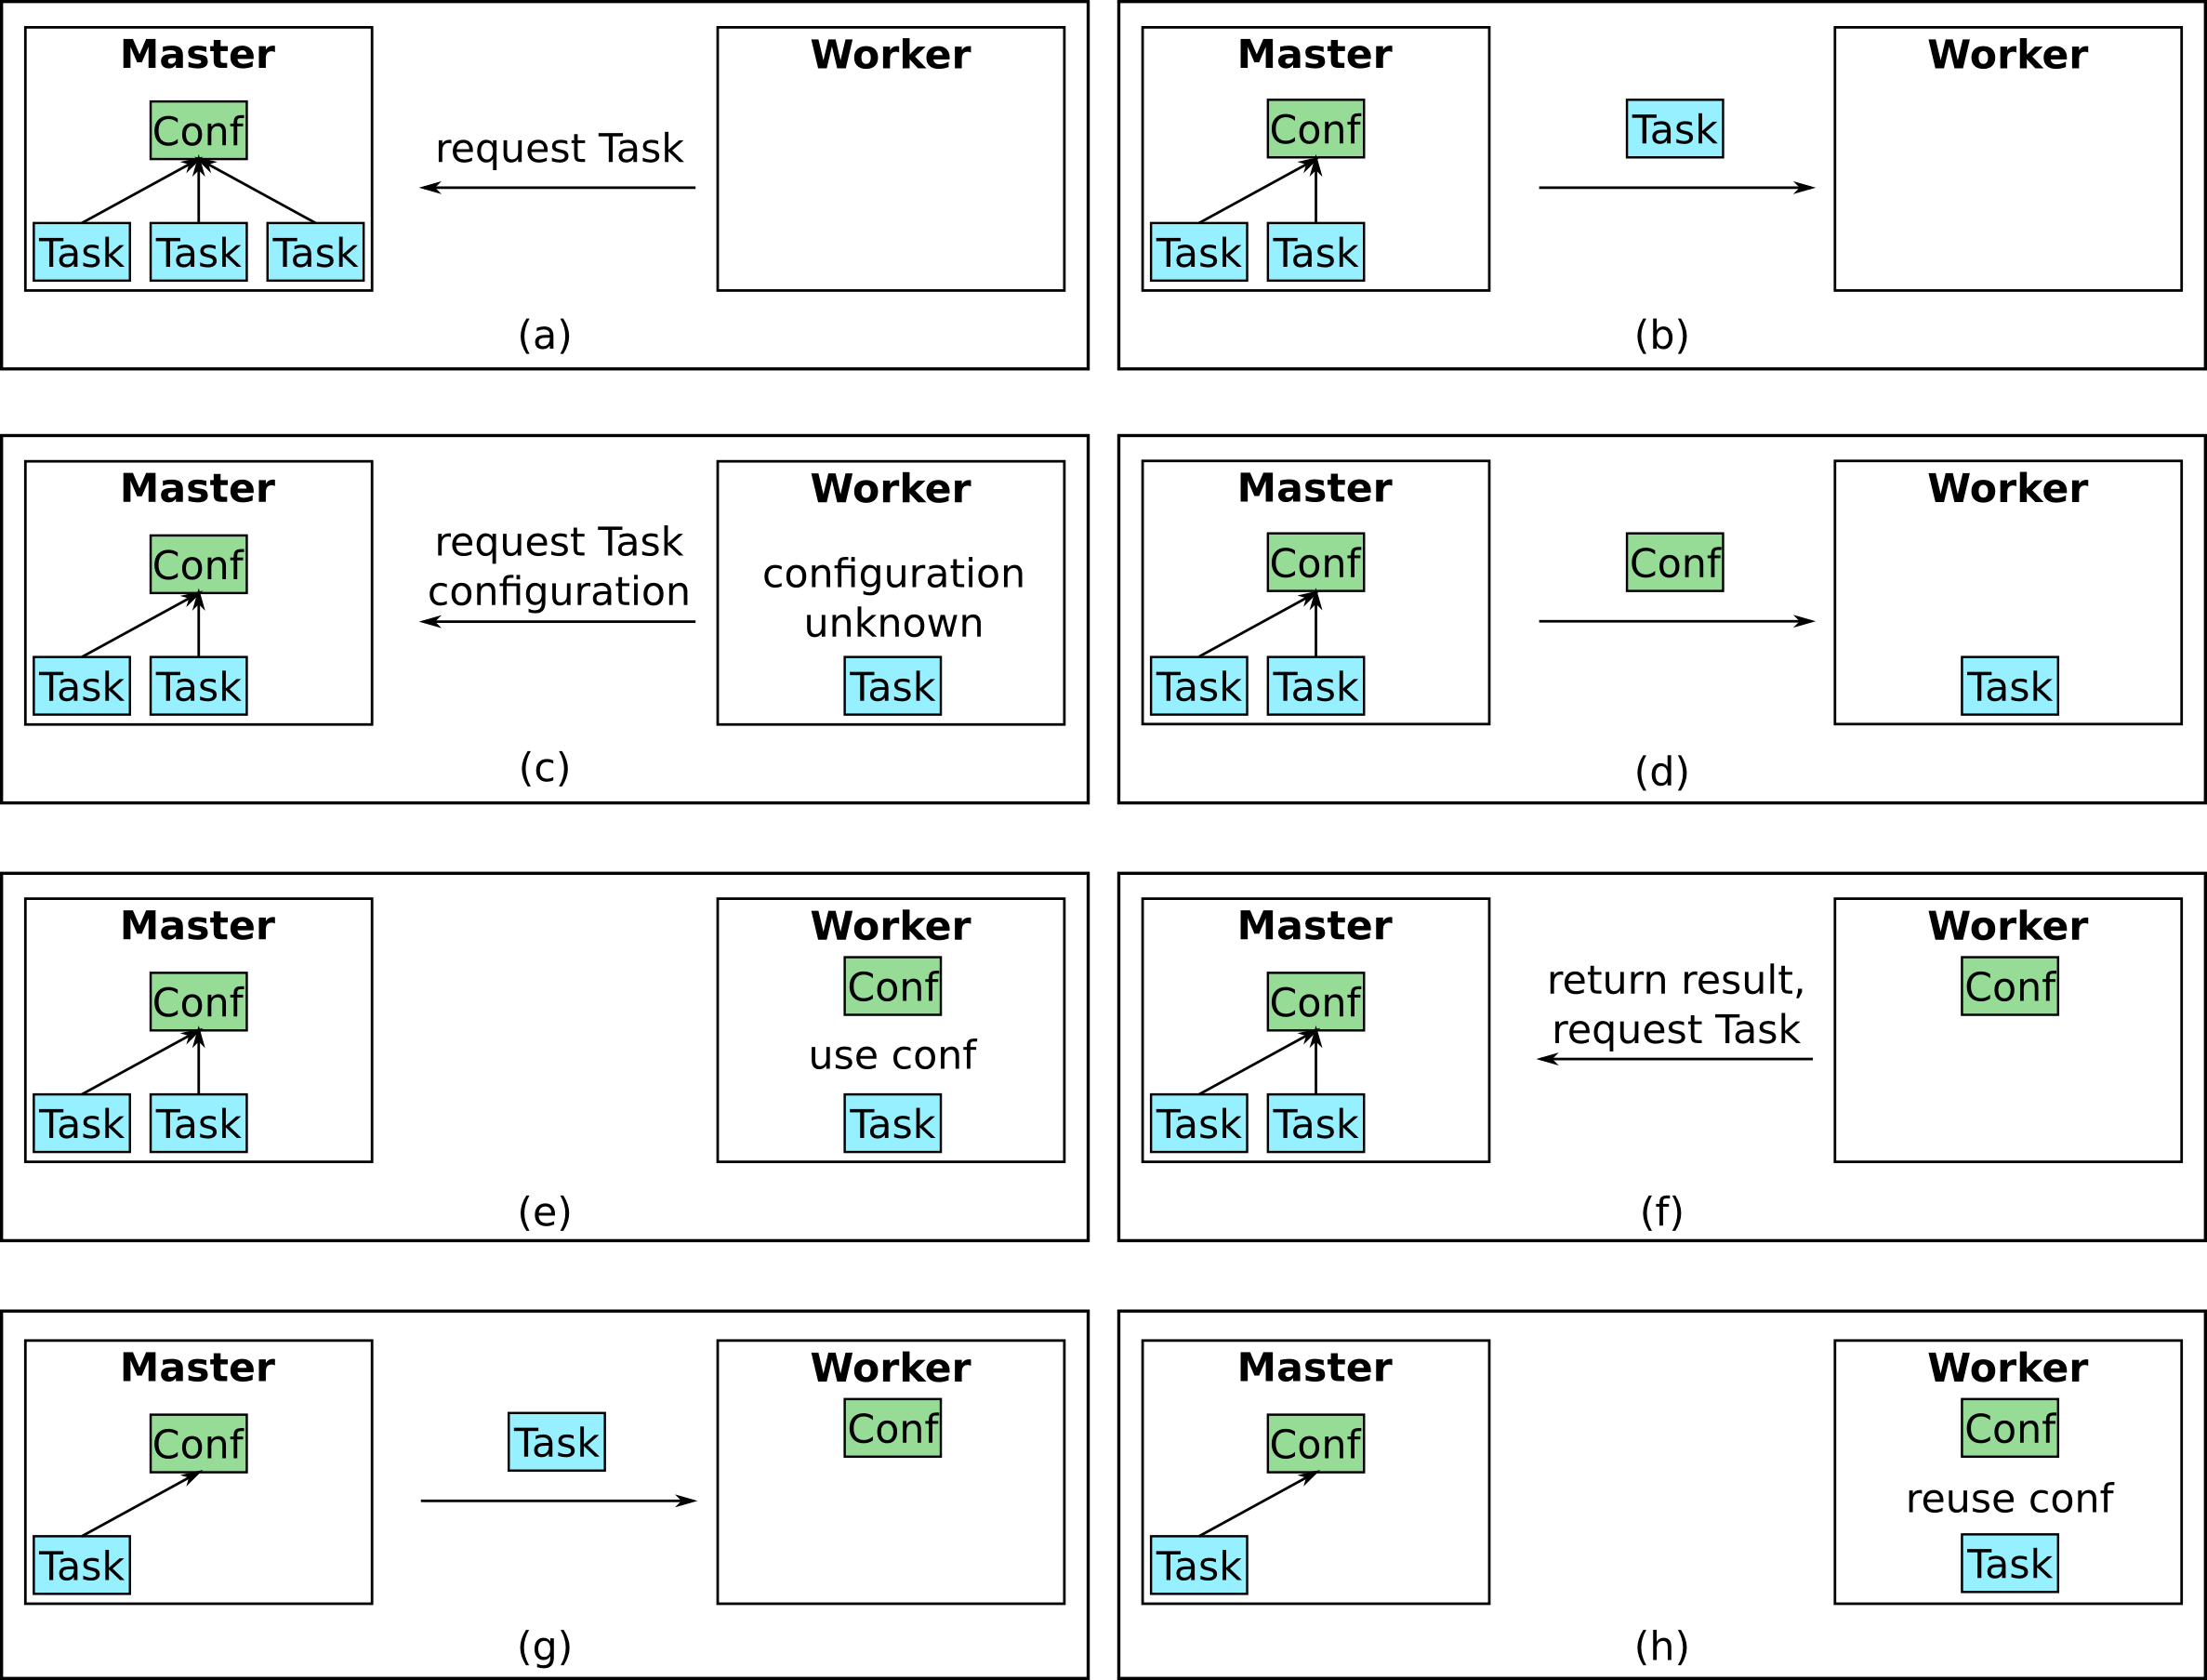
\includegraphics[width=130mm]{task-conf-reuse.png}
  \caption{A worker requests tasks from the master. The task configuration is send to the worker on demand.}
  \label{fig:task-conf-reuse}
\end{figure}

More details about the task system can be found in section \ref{chap:impl:task-system}

Persistence is another feature provided by Biohadoop. It can be used to save and load arbitrary data sets to and from the file system. This is convenient in many cases, for example if an algorithm wants to save its current state and reload this state at the next startup. To get more information about the persistence, refer to section \ref{chap:impl:persistence}.

Biohadoop is capable of running several algorithms at the same time in a single Biohadoop instance. They all run in the same JVM as Biohadoop does, and can be of arbitrary type. For example it is possible to run two GA instances and one PSO instance at the same time. As YARN doesn't guarantee when an application runs, the mentioned capability of launching several algorithms at the same time in the same JVM is a useful enhancement when it comes to high level parallelization using the island model, as it guarantees that the algorithms really run at the same time. If the algorithms are started as separate Biohadoop instances, it is possible that they run in sequential order, instead of running at the same time.

But Biohadoop doesn't restrict the usage of the island model to algorithms that run in the same JVM. By taking advantage of ZooKeeper \cite{zookeeper}, running algorithms find each other also across the boundaries of different Biohadoop instances. This can lead to higher scalability, as each instance gets its own resources, but entails the aforementioned problem that YARN doesn't guarantee when an application runs, so a trade off has to be made. More information about how to use the island model in Biohadoop can be found in section \ref{chap:impl:island-model}.

Biooozie (section \ref{chap:impl:oozie}) implements a custom action for Apache Oozie and is used to run Biohadoop as part of a larger workflow. The action schedules a single Biohadoop instance or several instances in parallel, depending on its configuration.

The following sections in this chapter continue to describe the details of Biohadoop in more detail, starting with the notion of Algorithm in section \ref{chap:impl:algorithm}. Section \ref{chap:impl:task-system} talks about the task system and its components, followed by the description of the communication mechanisms in section \ref{chap:impl:communication}. The enhancements section \ref{chap:impl:enhancements} provides information about Biohadoops support for persistence and the island model. Section \ref{chap:impl:configuration} explains how to configure Biohadoop. Biooozie is presented in the section \ref{chap:impl:oozie} of this chapter. Information on how to use Biohadoop can be found in chapter \ref{chap:usage}.

\section{Algorithm}
\label{chap:impl:algorithm}
An algorithm in terms of Biohadoop is the implementation of an abstract problem that should be solved. For example, a genetic algorithm (GA) can be implemented to solve an optimization problem.

Biohadoop supports the programmer with an easy way to parallelize the algorithm by providing the asynchronous task system (see \ref{chap:impl:task-system}). The algorithm can submit tasks to the task system and the task system takes care about the distribution and computation of the tasks and promotes the results back to the algorithm. The technical details of the task system are hidden from the algorithm.

Additional mechanisms that are offered to algorithms include persistence and high level parallelization using an island model (see \ref{chap:impl:enhancements}).

All those capabilities can be used by the algorithm, but Biohadoop does not force their usage. The only thing an algorithm has to do to be run by Biohadoop, is to implement the \texttt{Algorithm} interface. This interface defines one method, namely \texttt{run}, which is invoked by Biohadoop after the system initialization has completed. The return value of the \texttt{run} method is void as there is no return data that could be used in a general way. This may change in future versions.

It is possible to run several algorithms of any kind at the same time in one Biohadoop instance (for example two GA and one PSO), this is just a matter of configuration (see section \ref{chap:impl:configuration}).
   
If there is an error during the execution of an algorithm, the algorithm may throw a \texttt{AlgorithmException} at any time. The meaning of a thrown \texttt{AlgorithmException} is, that there was an unrecoverable error which prevented the algorithm from progress, but the programmer was aware that such an error could happen, e.g. when a needed configuration argument is missing. Sometimes an algorithm may throw an unchecked exception, like the \texttt{NullPointerException}. The difference to the \texttt{AlgorithmException} lies in the semantics: unchecked exceptions are considered as the outcome of bugs. At the moment, Biohadoop makes no difference in handling \texttt{AlgorithmException} and unchecked exceptions, in both cases, the error is logged and the algorithm is terminated without affecting other running algorithms. But it is possible that this behavior may change in the future. For example, it is thinkable that a custom recovery procedure is invoked in case of an \texttt{AlgorithmException}.

\section{Task system}
\label{chap:impl:task-system}
If a programmer decides to parallelize some parts of an algorithm, it can use Biohadoops task system. The task system takes care of promoting tasks to waiting workers and to return the results to the algorithm, while hiding the details of this process from the algorithm.

The task system consists of a task broker, at least one endpoint and at least one worker. The broker and endpoints are executed on the master, which is the ApplicationMaster in YARN. The workers are executed in additional YARN containers.

An algorithm submits its tasks to the task system, by adding them directly to the broker or by using the \texttt{TaskSubmitter}. It is advised to use the the \texttt{TaskSubmitter}, as it offers a simple interface for task submission, while the broker offers additional methods that are needed internally by the task system. When an algorithm submits a task, it immediately receives back a \texttt{TaskFuture} that works similar to the Java \texttt{Future}. The \texttt{TaskFuture} represents the result of the task computation. The attempt to read the result of a task computation from a \texttt{TaskFuture} has two possible outcomes. In the first case, the result is known and can be read from the \texttt{TaskFuture}. In the second case, the result is yet not known (because it still needs to be computed) and the read attempt blocks until the result is available. In addition to the possibly blocking read, the \texttt{TaskFuture} provides a non blocking method to check if the \texttt{TaskFuture} contains a result.

A queued task is eventually taken out of the broker by an endpoint. Endpoints represent a boundary between the broker on the master side and the workers on the other side. They interact with the broker and communicate with the workers. On worker request, an endpoint takes the next task out of the broker and sends it to the worker. The worker computes the result for the task, using the task data and its related task configuration, and returns the result to an endpoint. The endpoint then returns the result to the task broker, which promotes it back to the algorithm. Figure \ref{fig:task-system} gives a graphical representation of this procedure.

The task system works in an asynchronous manner and doesn't block the algorithm while processing the tasks. However, it provides also mechanisms to block and wait for a result to be computed, if this is preferred.

\begin{figure}[ht!]
  \centering
  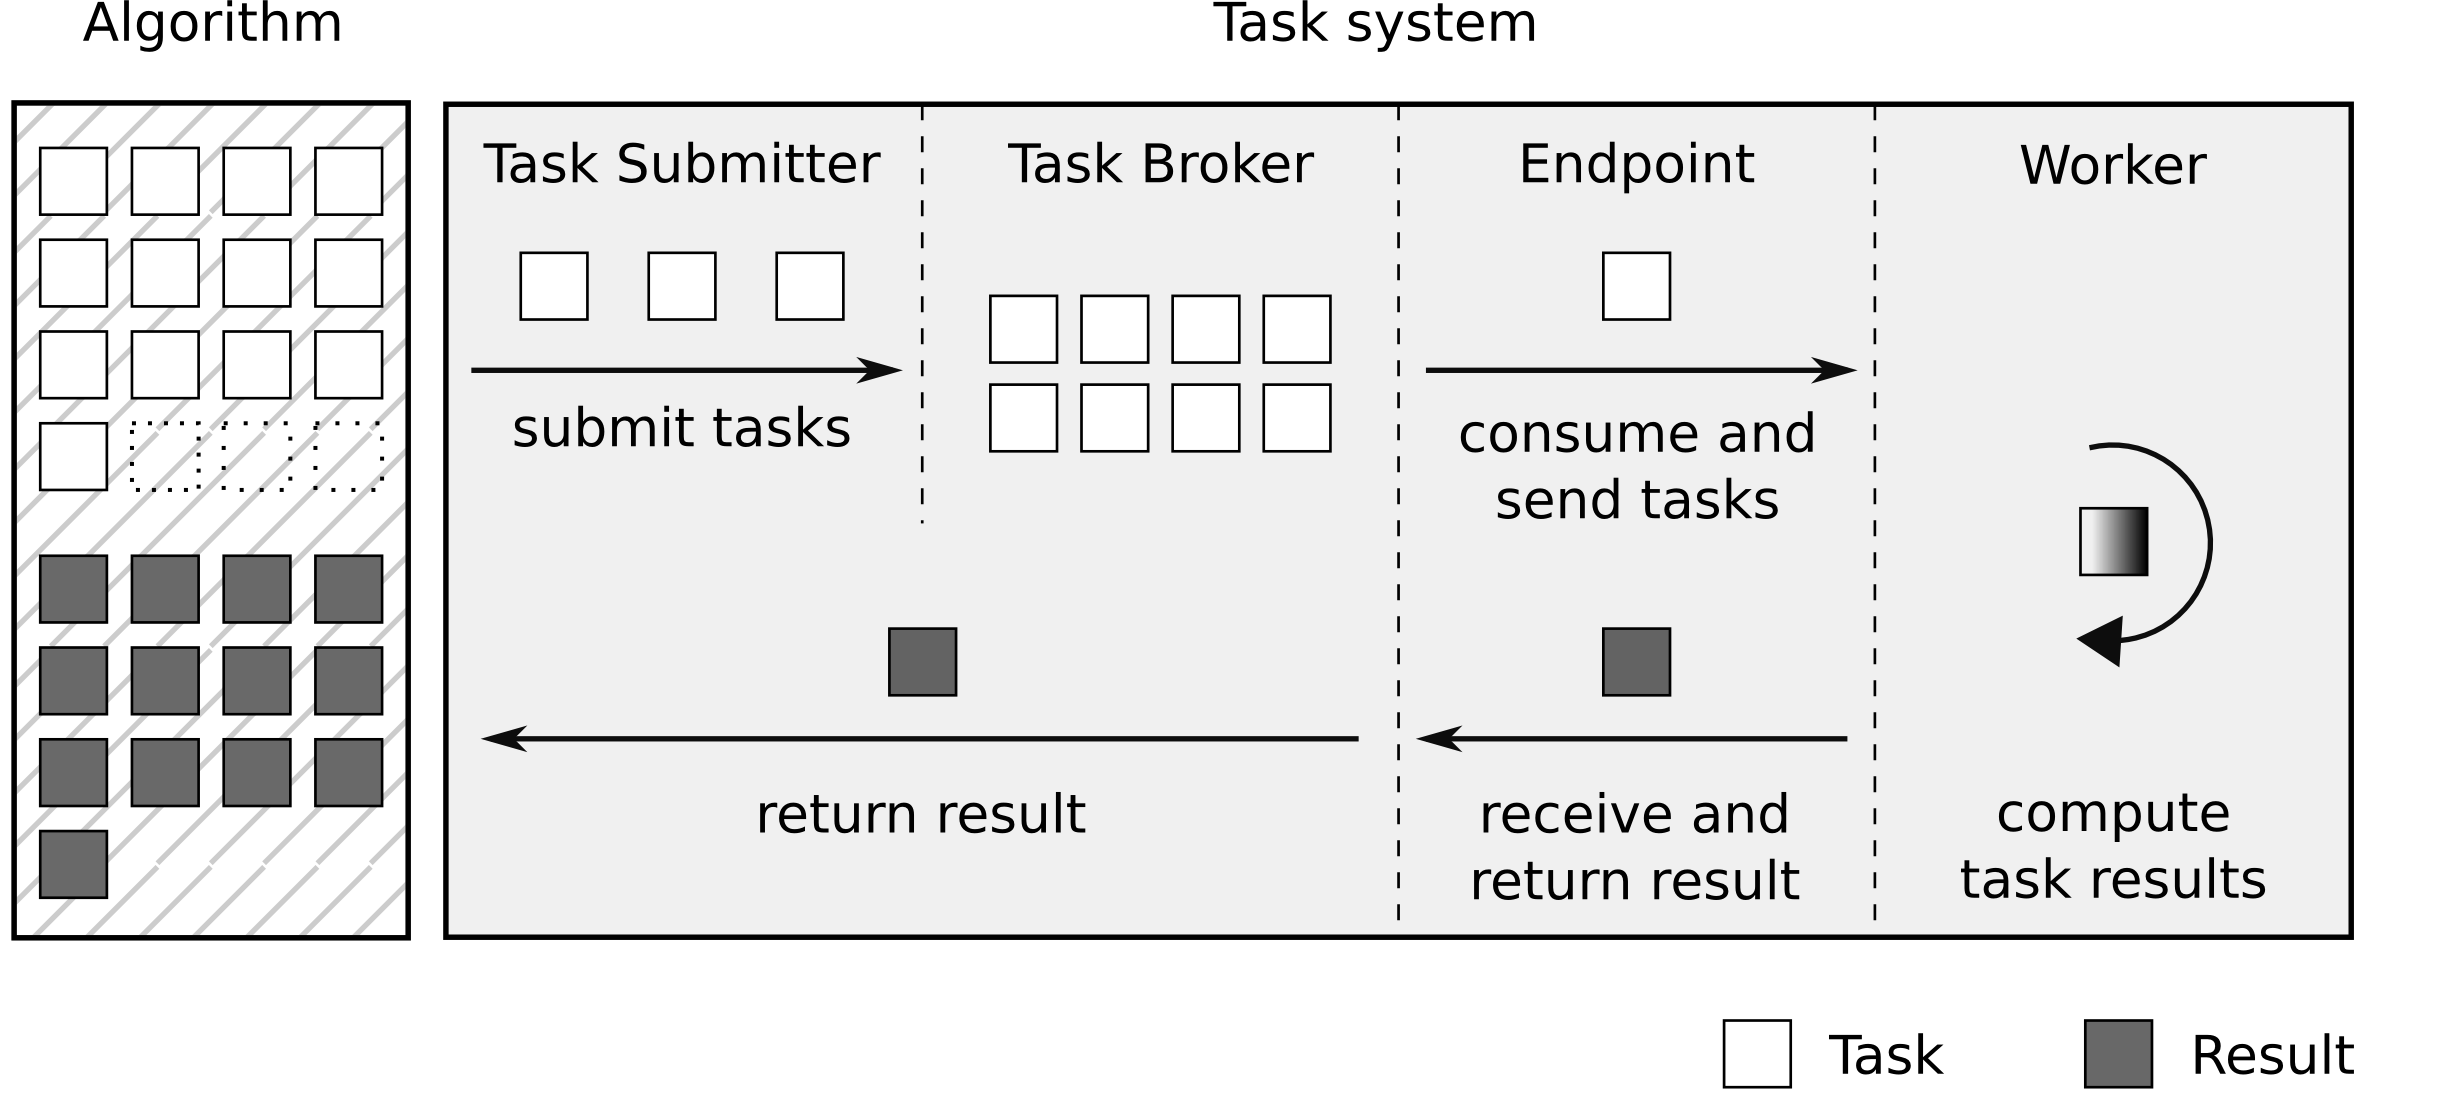
\includegraphics[width=130mm]{task-system.png}
  \caption{Submitting tasks to the task system. The task system consists of a task broker and any number of endpoints and workers. For the sake of simplicity, the figure shows only one endpoint and one worker. In this figure, an optional task submitter is used for task submission.}
  \label{fig:task-system}
\end{figure}

\subsection{Task Broker}
The task broker is the central feature in the task system, it is used to exchange tasks and their results between the algorithms and the endpoints. The broker combines an internal FIFO queue with additional task bookkeeping (see the concepts below).

All submitted tasks reference a task configuration that is used by the workers to compute the task result. This configuration can be shared by any number of tasks. The configuration reference for a given task is stored in the task broker. The configuration itself is send to the workers on demand. A worker requests a specific task configuration, if it encounters a task whose configuration is unknown to the worker. After the configuration was received, it is cached by the worker for later reuse. This is appropriate as usually many tasks use the same configuration. In the GA example, where the workers generate offsprings and compute their fitness values, a single task configuration is enough for all tasks, as offspring generation and fitness evaluation is done in the same way for all tasks. Therefore, a worker needs to obtain the task configuration only once, reducing the communication overhead. It is of course also possible to assign each task an individual task configuration. The result would be, that the worker has to request the configuration for each task individually, the communication overhead would be much higher than in the previous example.

To work properly, the task broker uses two concepts that are needed to perform its work. 

The first concept is its internal first-in first-out (FIFO) queue, that stores the submitted tasks. The FIFO queue is thread safe, to allow multiple producers (algorithms) and consumers (endpoints) to interact with the queue at the same time. As an example, lets suppose that two GAs are running in one Biohadoop instance. Both algorithms can submit new tasks, while the endpoints consume tasks from the broker. By using a thread safe FIFO queue, all of this can happen at the same time, without causing problems.

The second concept is a map, that connects submitted tasks to their configuration and their \texttt{TaskFuture}. This must be done, because a task loses its references once it is taken out of the FIFO queue and send to a worker. The configuration for the task would become unknown and the result of the task could no longer be associated with the corresponding \texttt{TaskFuture}. The mentioned map resolves this problem.

The two concepts are depicted in figure \ref{fig:task-broker}. In the first step, a task and its configuration is submitted to the broker. The broker inserts the task in its internal FIFO queue and adds the task, the configuration and a new \texttt{TaskFuture} to its internal map. The \texttt{TaskFuture} is immediately returned to the algorithm as result of the task submission. At this stage, any attempt to access the result of the \texttt{TaskFuture} would block, as the result of the task computation is unknown yet. At a certain point, step 2 is performed, where the queued task $T_N$ is consumed by an endpoint and send to a waiting worker. If the worker doesn't know about the referenced configuration $TC_N$ for task $T_N$, it asks the endpoint for the configuration, which gets the configuration from the broker in step 3. The configuration for the task $T_N$ can only be retrieved, because the broker kept a reference to it in its internal map. In step 4, the worker returns the computed result to the endpoint, which forwards it to the broker. The broker associates the result for task $T_N$ with the according \texttt{TaskFuture} $TF_N$, again using its internal map. After the result for the \texttt{TaskFuture} is set, the algorithm can access the result for task $T_N$ without blocking.

\begin{figure}[ht!]
  \centering
  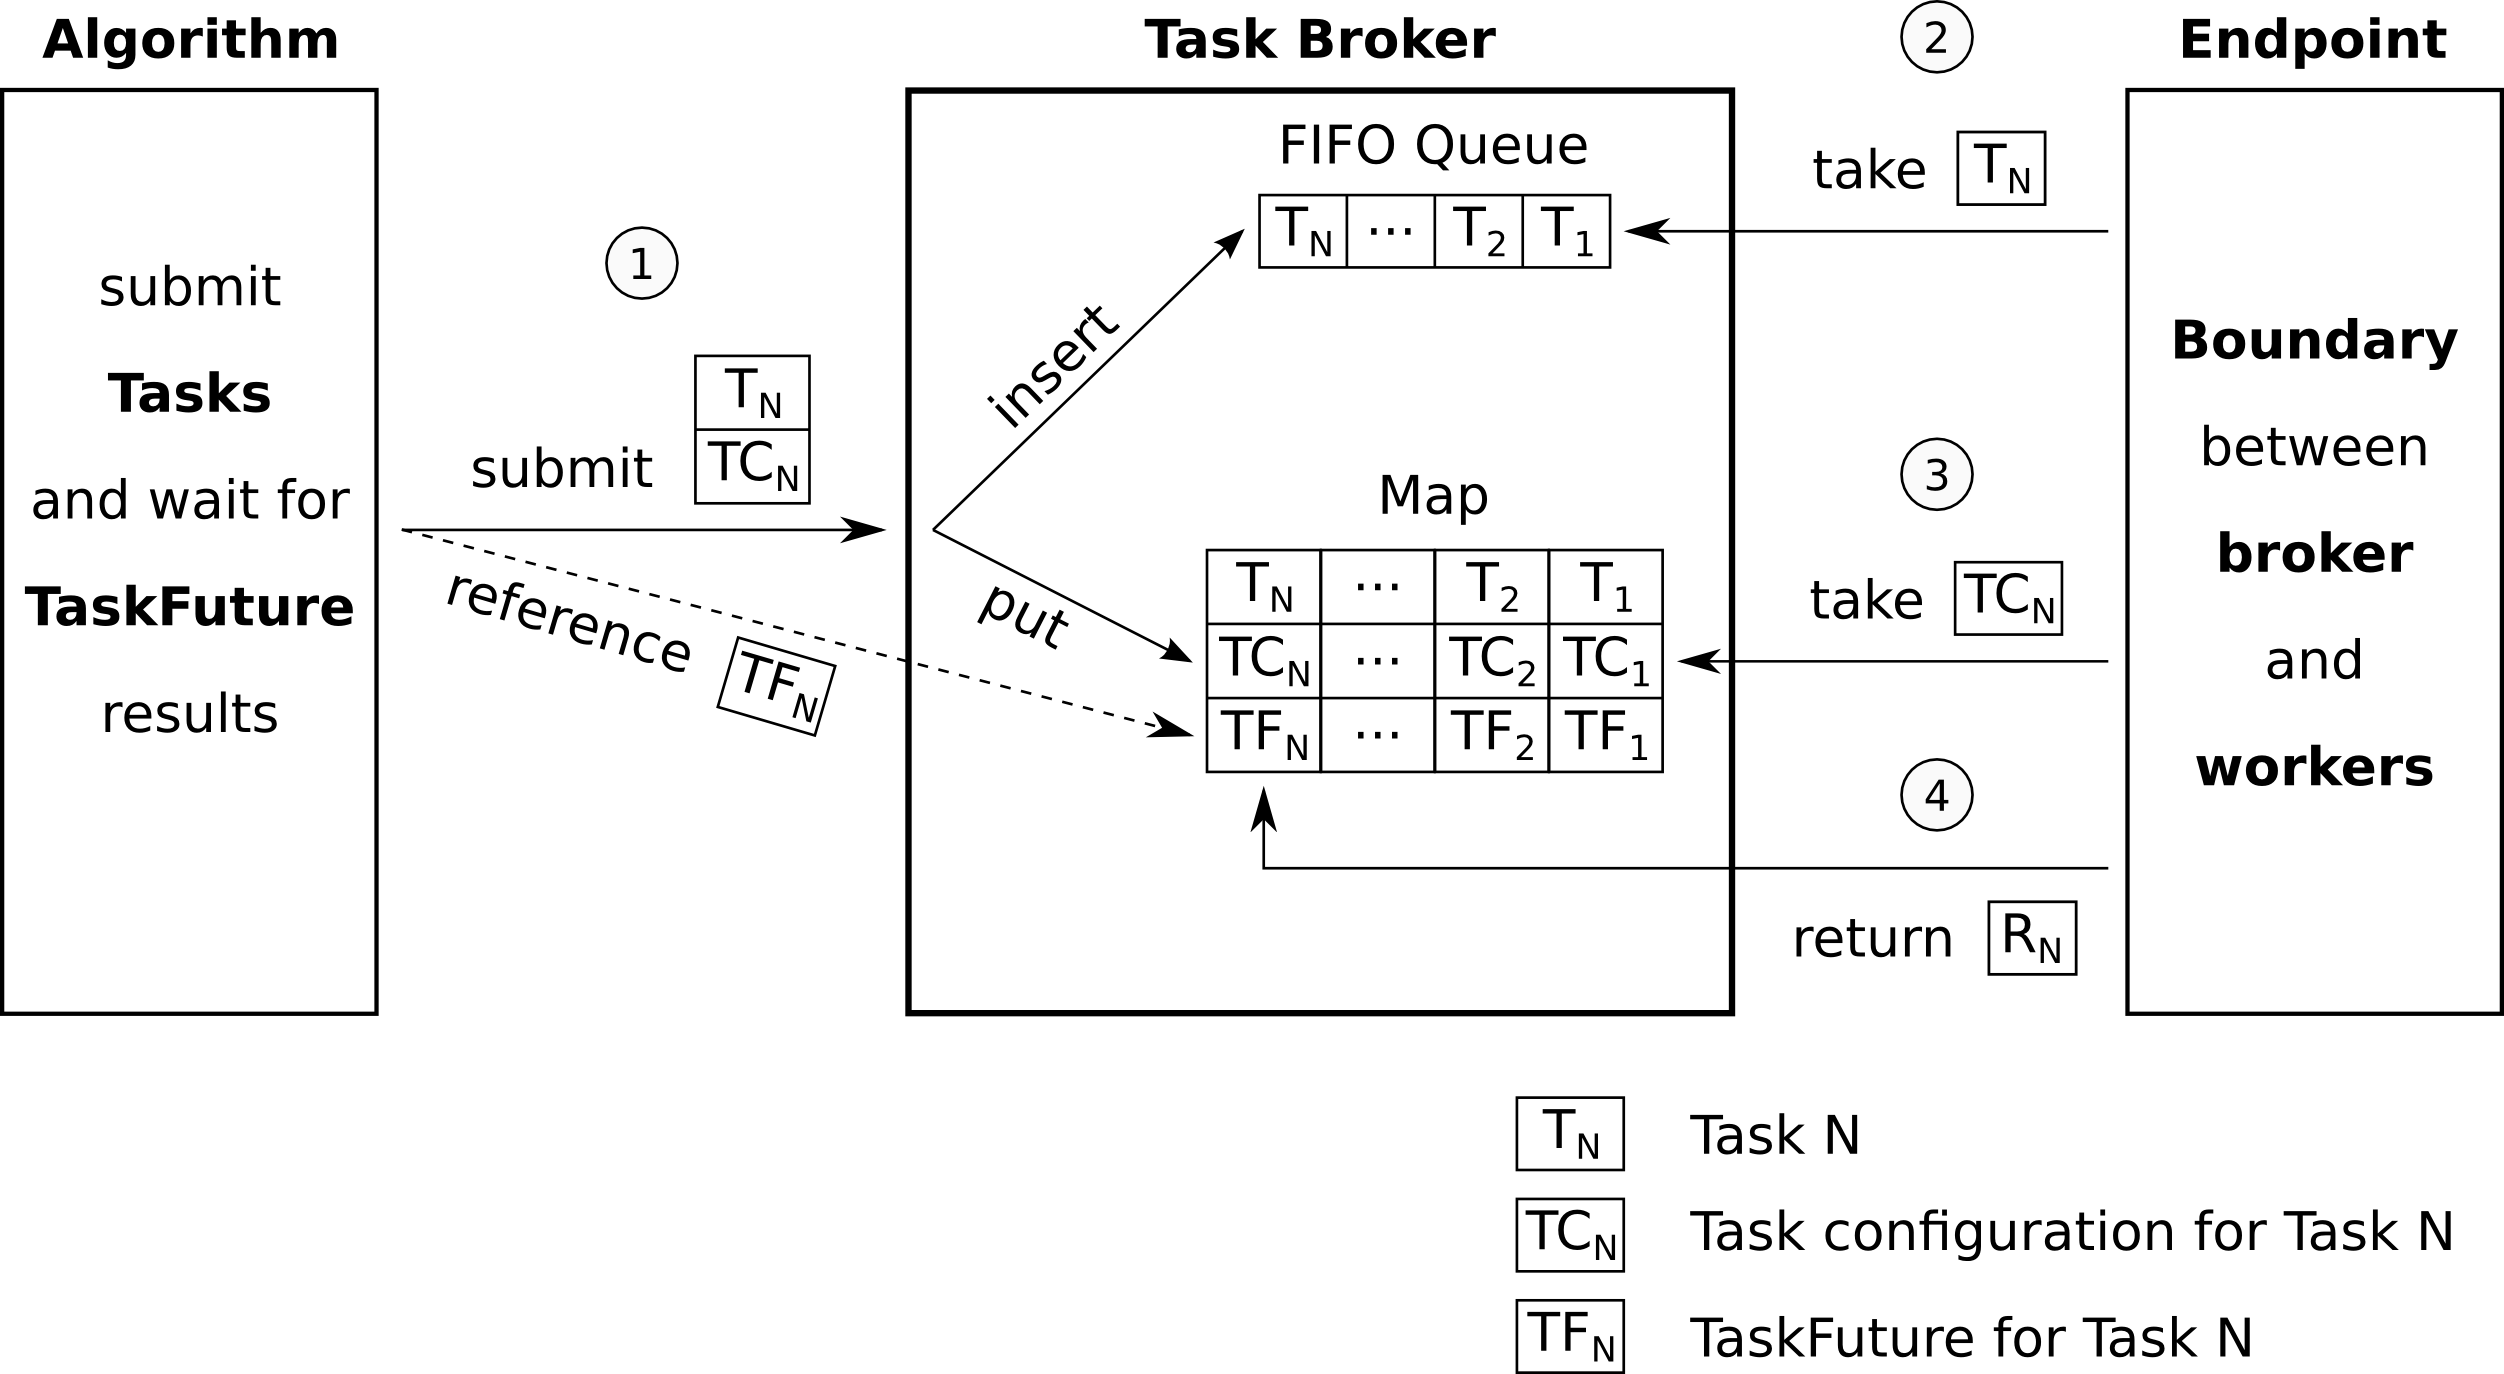
\includegraphics[width=130mm]{task-broker.png}
  \caption{Internal structure of the task broker}
  \label{fig:task-broker}
\end{figure}

In addition to task and result exchange, the task broker provides methods to resubmit a task. This is needed in the case of a failure during the computation of the task result.

\subsection{Endpoint}
\label{chap:impl:endpoint}
An endpoint is a boundary between the task broker and the workers. It's main purpose is the communication with the workers. By hiding the technical details of the communication from the algorithm and the task broker, any type of communication facility between the master and the workers can be implemented. This property lead to the implementation of two different communication protocols for Biohadoop. Section \ref{chap:impl:communication} talks in greater detail about the communication.

Communication is not the only purpose of an endpoint. It interacts also with the task broker, taking tasks and task configurations out of it or returning results that were received from the workers. The attempt of an endpoint to get a task from the broker blocks, if the brokers internal FIFO queue is empty. As soon as new tasks are available, the endpoint continues to work. A blocked endpoint blocks also its waiting workers.

An endpoint is allowed to resubmit a task to the task broker, if there is the need to. For example, lets suppose a task is taken from the task broker and send to a worker. This worker encounters a problem and terminates before returning the result. The endpoint can detect the issue with different methods (e.g. connection closed, heartbeat, time out, etc.) and resubmit the task to the task broker. This way, no task gets lost.

It is possible to run an arbitrary amount of endpoints, but usually this is not necessary. Nevertheless, it can be useful to run different endpoints for different communication protocols (see section \ref{chap:impl:communication}).

The endpoints run in the YARN ApplicationMaster and are started and stopped automatically by Biohadoop. It is configurable which endpoints should be started, section \ref{chap:impl:configuration} gives details about the configuration aspects.

\subsection{Worker}
\label{chap:impl:worker}
A worker computes the result for a given task using the configuration that is referenced by the task. The task itself contains the data needed for the computation. The configuration contains information about how to compute the result for the task. The ``how'' is specified by a Java class that implements the \texttt{AsyncComputable} interface. In addition, the task configuration can contain an immutable data set, shared by all tasks that reference the same configuration. The immutable data set is called  ``initial data''.

In the GA example, a task generates and evaluates an offspring. The task data consists of the parent individuals and the task configuration points to a class that implements offspring generation and fitness evaluation. The ``initial data'' contains static parameters for offspring creation and fitness evaluation. The worker uses the configuration to instantiate the given \texttt{AsyncComputable} class. The class and the ``initial data'' are then used to compute the result for the task, which is a new offspring and its related fitness value. The result is then send to the endpoint.

Tasks are send to the workers without task configuration. The task configuration is delivered only on demand and is afterwards cached by the worker. This can be done, as most tasks will share a common configuration. Sending the configuration only on demand, reduces the amount of transmitted data and increases therefore the performance of the whole system. Figure \ref{fig:async-computable} shows how tasks and task configurations are handled by the workers.

\begin{figure}[ht!]
  \centering
  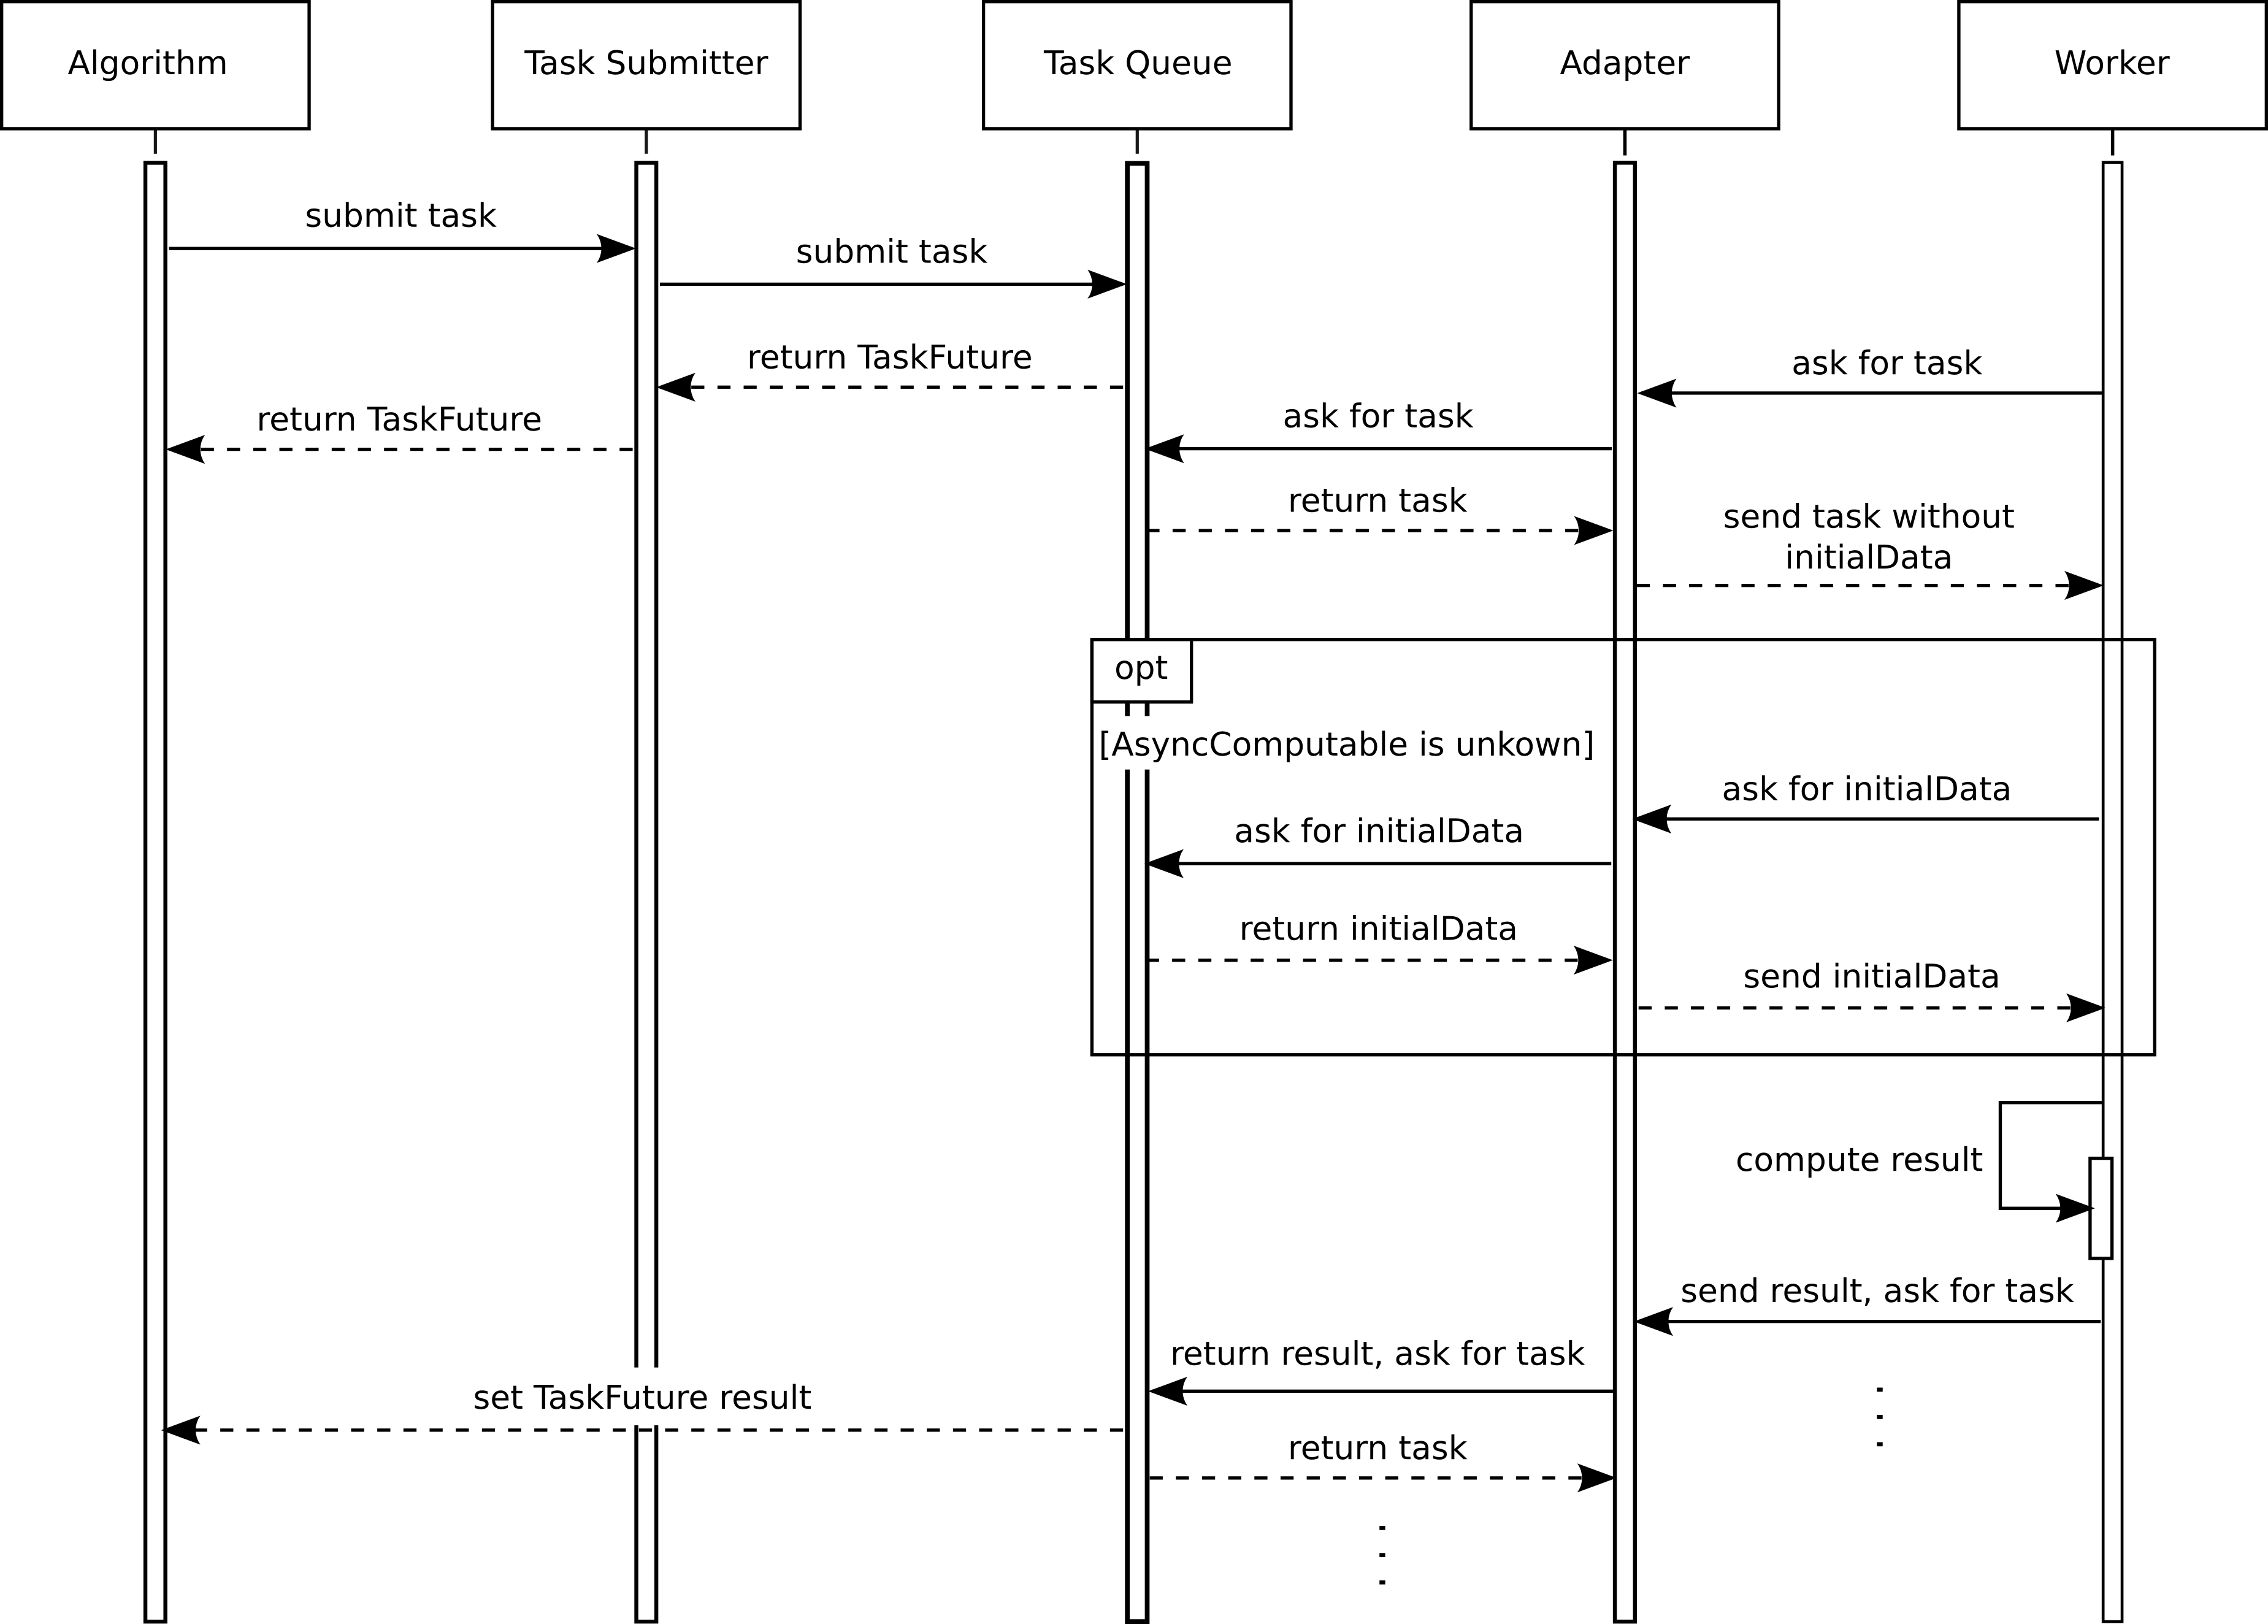
\includegraphics[width=130mm]{flow-asyncComputable.png}
  \caption{Life cycle of a task, the result is computed by a worker using an AsyncComputable}
  \label{fig:async-computable}
\end{figure}

A worker needs to communicate with an endpoint to get tasks. If the endpoint has currently no work to offer, for example because the running algorithms have not submitted any tasks to the task system, then the worker waits until new work is available. Of course the worker need some resources during the waiting times too, like CPU, RAM and storage or, in YARN terms, containers. One should consider and measure how many workers are really needed.

Biohadoop supports two different kinds of workers: the ones that run under the control of the Apache Hadoop system (from now on called embedded workers) and the ones that run outside of this system (from now on called external workers).

Embedded workers must be configured in Biohadoop, which controls their life cycle. In contrast, external workers can not be configured by Biohadoop, their whole life cycle must be controlled in some other way that is not part of Biohadoop. This can pose some problems, as external workers need to know e.g. when and where Biohadoop is running. The solution to this problems is outside of the scope of this thesis.

If there are no special needs, embedded workers are just fine. There are although some good reasons to use external workers:

\begin{itemize}
  \item external worker don't necessarily depend on the Hadoop ecosystem, they may run wherever they want, as long as they are able to communicate to at least one endpoint. It is possible to develop external workers that run in completely different environments, for example on mobile phones.
  \item there is no restriction on the program language for an external worker, as long as it knows how to talk to an endpoint. For example it is possible to implement a worker in JavaScript \cite{bioworker-browser} or Python \cite{bioworker-python}. In contrast to this, embedded workers have to be written in Java.
  \item there is no limit to the number of external workers that may run. On the other side, the number of embedded workers is limited by the Hadoop environment on which Biohadoop runs.
\end{itemize}

Biohadoop provides the possibility to run different endpoints to support external workers. The endpoints may implement arbitrary communication protocols, e.g. WebSockets with JSON serialization for external workers written in JavaScript.

\section{Communication}
\label{chap:impl:communication}
The communication between the algorithms, the broker and the endpoints is not difficult, as they run in the YARN ApplicationMaster and therefore in the same JVM. It is just a matter of sharing variables between the different threads, possibly protected by concurrency protocols. For example, the task broker contains a FIFO queue based on the Java \texttt{LinkedBlockingQueue}, which is a thread safe queue that supports concurrent writers and readers.
  
Communicating between endpoints and workers is more complicated, as the endpoints and workers may run in different processes or even on different machines, so variable sharing is not that easy. A more sophisticated communication method must be used.

Biohadoop uses Netty \cite{netty} for all communication purposes that span different processes or machines. Netty is a high performance framework for network applications that hides the underlying socket implementation from the user and provides a useful and well tested API to build distributed applications. Netty provides TCP and UDP support, only TCP is used for Biohadoop. All provided endpoints and workers use Netty as their communication base.

The communication protocols on top of Netty can be of arbitrary type. Biohadoop provides two implementations for endpoints and workers that use sockets (hidden by Netty) or the WebSocket protocol. The socket protocol uses Kryo \cite{kryo} for object serialization, while the WebSocket protocol relies on JSON serialization. The two protocols are discussed in more detail in section \ref{chap:impl:protocols}.

The reason for the support of different protocols lies in their different use cases. While the performance of sockets with Kryo serialization is higher than for WebSockets, WebSockets have the advantage of great compatibility and broad support in different languages. This is important for external workers as they don't have to be implemented in Java.

On top of the communication protocols, Biohadoop establishes its own application protocol for task, configuration and result exchange between endpoints and workers. This protocol defines a communication flow further described in section \ref{chap:impl:communication-flow}. Figure \ref{fig:communication-layers} shows the different layers that Biohadoop uses for data exchange.

\begin{figure}[ht!]
  \centering
  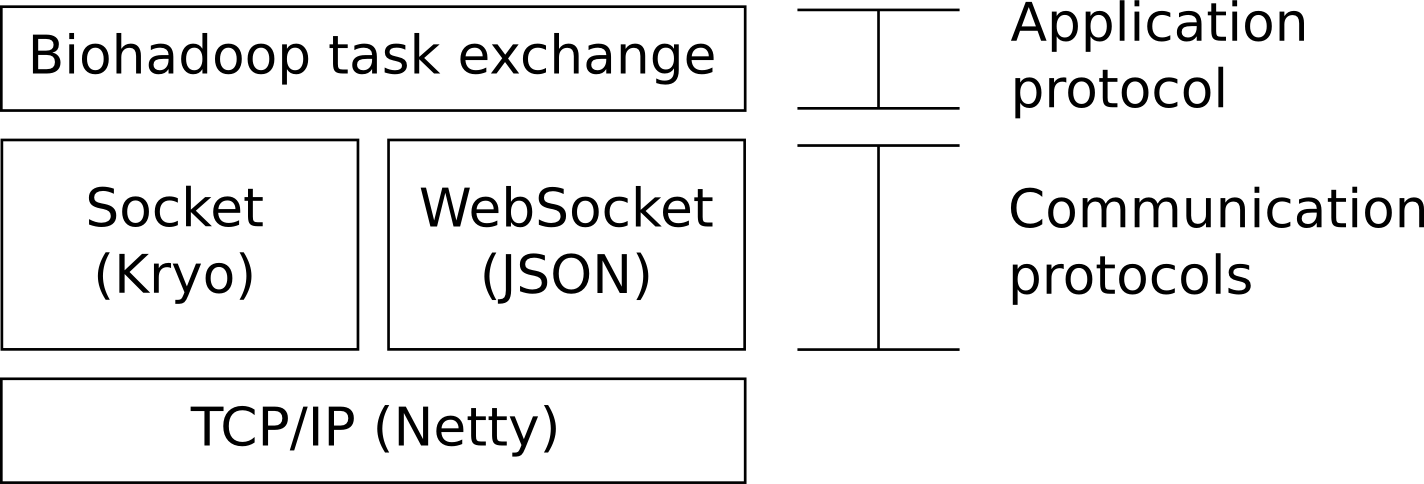
\includegraphics[width=80mm]{communication-layers.png}
  \caption{Biohadoops communication layers}
  \label{fig:communication-layers}
\end{figure}

Biohadoop enables the use of custom protocols, by implementing the appropriate parts of \texttt{Endpoint} and \texttt{Worker} interfaces. Corresponding endpoints and workers have to agree about the communication and application protocol.

\subsection{Protocols}
\label{chap:impl:protocols}
In this section, the two provided communication protocols of Biohadoop are described, each one has its advantages and disadvantages.

\subsubsection{Sockets}
The socket communication between endpoints and workers is implemented on top of Netty that provides an abstraction of the underlying raw TCP/IP socket. The advantage of using Netty over raw sockets is, that Netty provides a simple to use API for non-blocking asynchronous communication. A manual implementation would have been more error prone.

Kryo \cite{kryo} is used for object serialization. It is a library for high speed serialization of Java objects and usually faster than the build-in serialization features of Java \cite{jvm-serializers}.

A disadvantage of Kryo is, that its object serialization is not a standard and therefore in broad usage. This restricts the worker implementations to be written in Java, which may not be a problem at all, especially if only embedded workers are used. But if external workers should be used, they have to be written in Java, or need to provide a custom Kryo implementation.

If the data exchanged between endpoints and workers is huge, the Kryo buffer sizes must be increased. This can be done by setting the according configuration options in the configuration file (see section \ref{chap:impl:configuration}).

\subsubsection{WebSocket}
The WebSocket implementation also uses Netty to hide the underlying TCP/IP socket. In contrast to the socket communication, it adds the WebSocket protocol on top of it. JSON is used for object serialization.

WebSockets are usually used for the communication between a web application and its application server. They rely on the HTTP protocol for the handshake, during which the communication partners agree to upgrade to the WebSocket protocol. After the upgrade is done, the communication between an endpoint and a worker can be performed using binary or text streams.

WebSockets have a very small overhead when data is exchanged, for example 2 byte for text stream messages. This is a major difference to the HTTP protocol where the HTTP headers are sent on each request and response. It improves the communication performance, especially for the transmission of small amounts of data. Another difference between WebSockets and HTTP is, that the WebSocket communication can be performed in full duplex, HTTP needs a request - response cycle. This can further improve the performance, but has no impact for Biohadoop, as the communication between endpoints and workers is performed in a request - response manner (see section \ref{chap:impl:communication-flow} for more information).

The biggest advantage of WebSockets and JSON lies in their standardization. This is important in combination with external workers, as those workers can be written in any language. Most languages have support for WebSockets and JSON - because they are standards. The biggest disadvantage of WebSockets with JSON is, that they are slower than sockets with Kryo serialization.

\subsection{Communication flow}
\label{chap:impl:communication-flow}
The communication protocols presented in the prior section are used as a base to the application protocol, that implements a well defined communication flow between endpoints and workers. This communication flow, depicted in figure \ref{fig:communication-flow}, is the same for both provided communication protocols. Custom protocols don't need to implement this flow, they are free to implement their own communication pattern.

\begin{figure}[ht!]
  \centering
  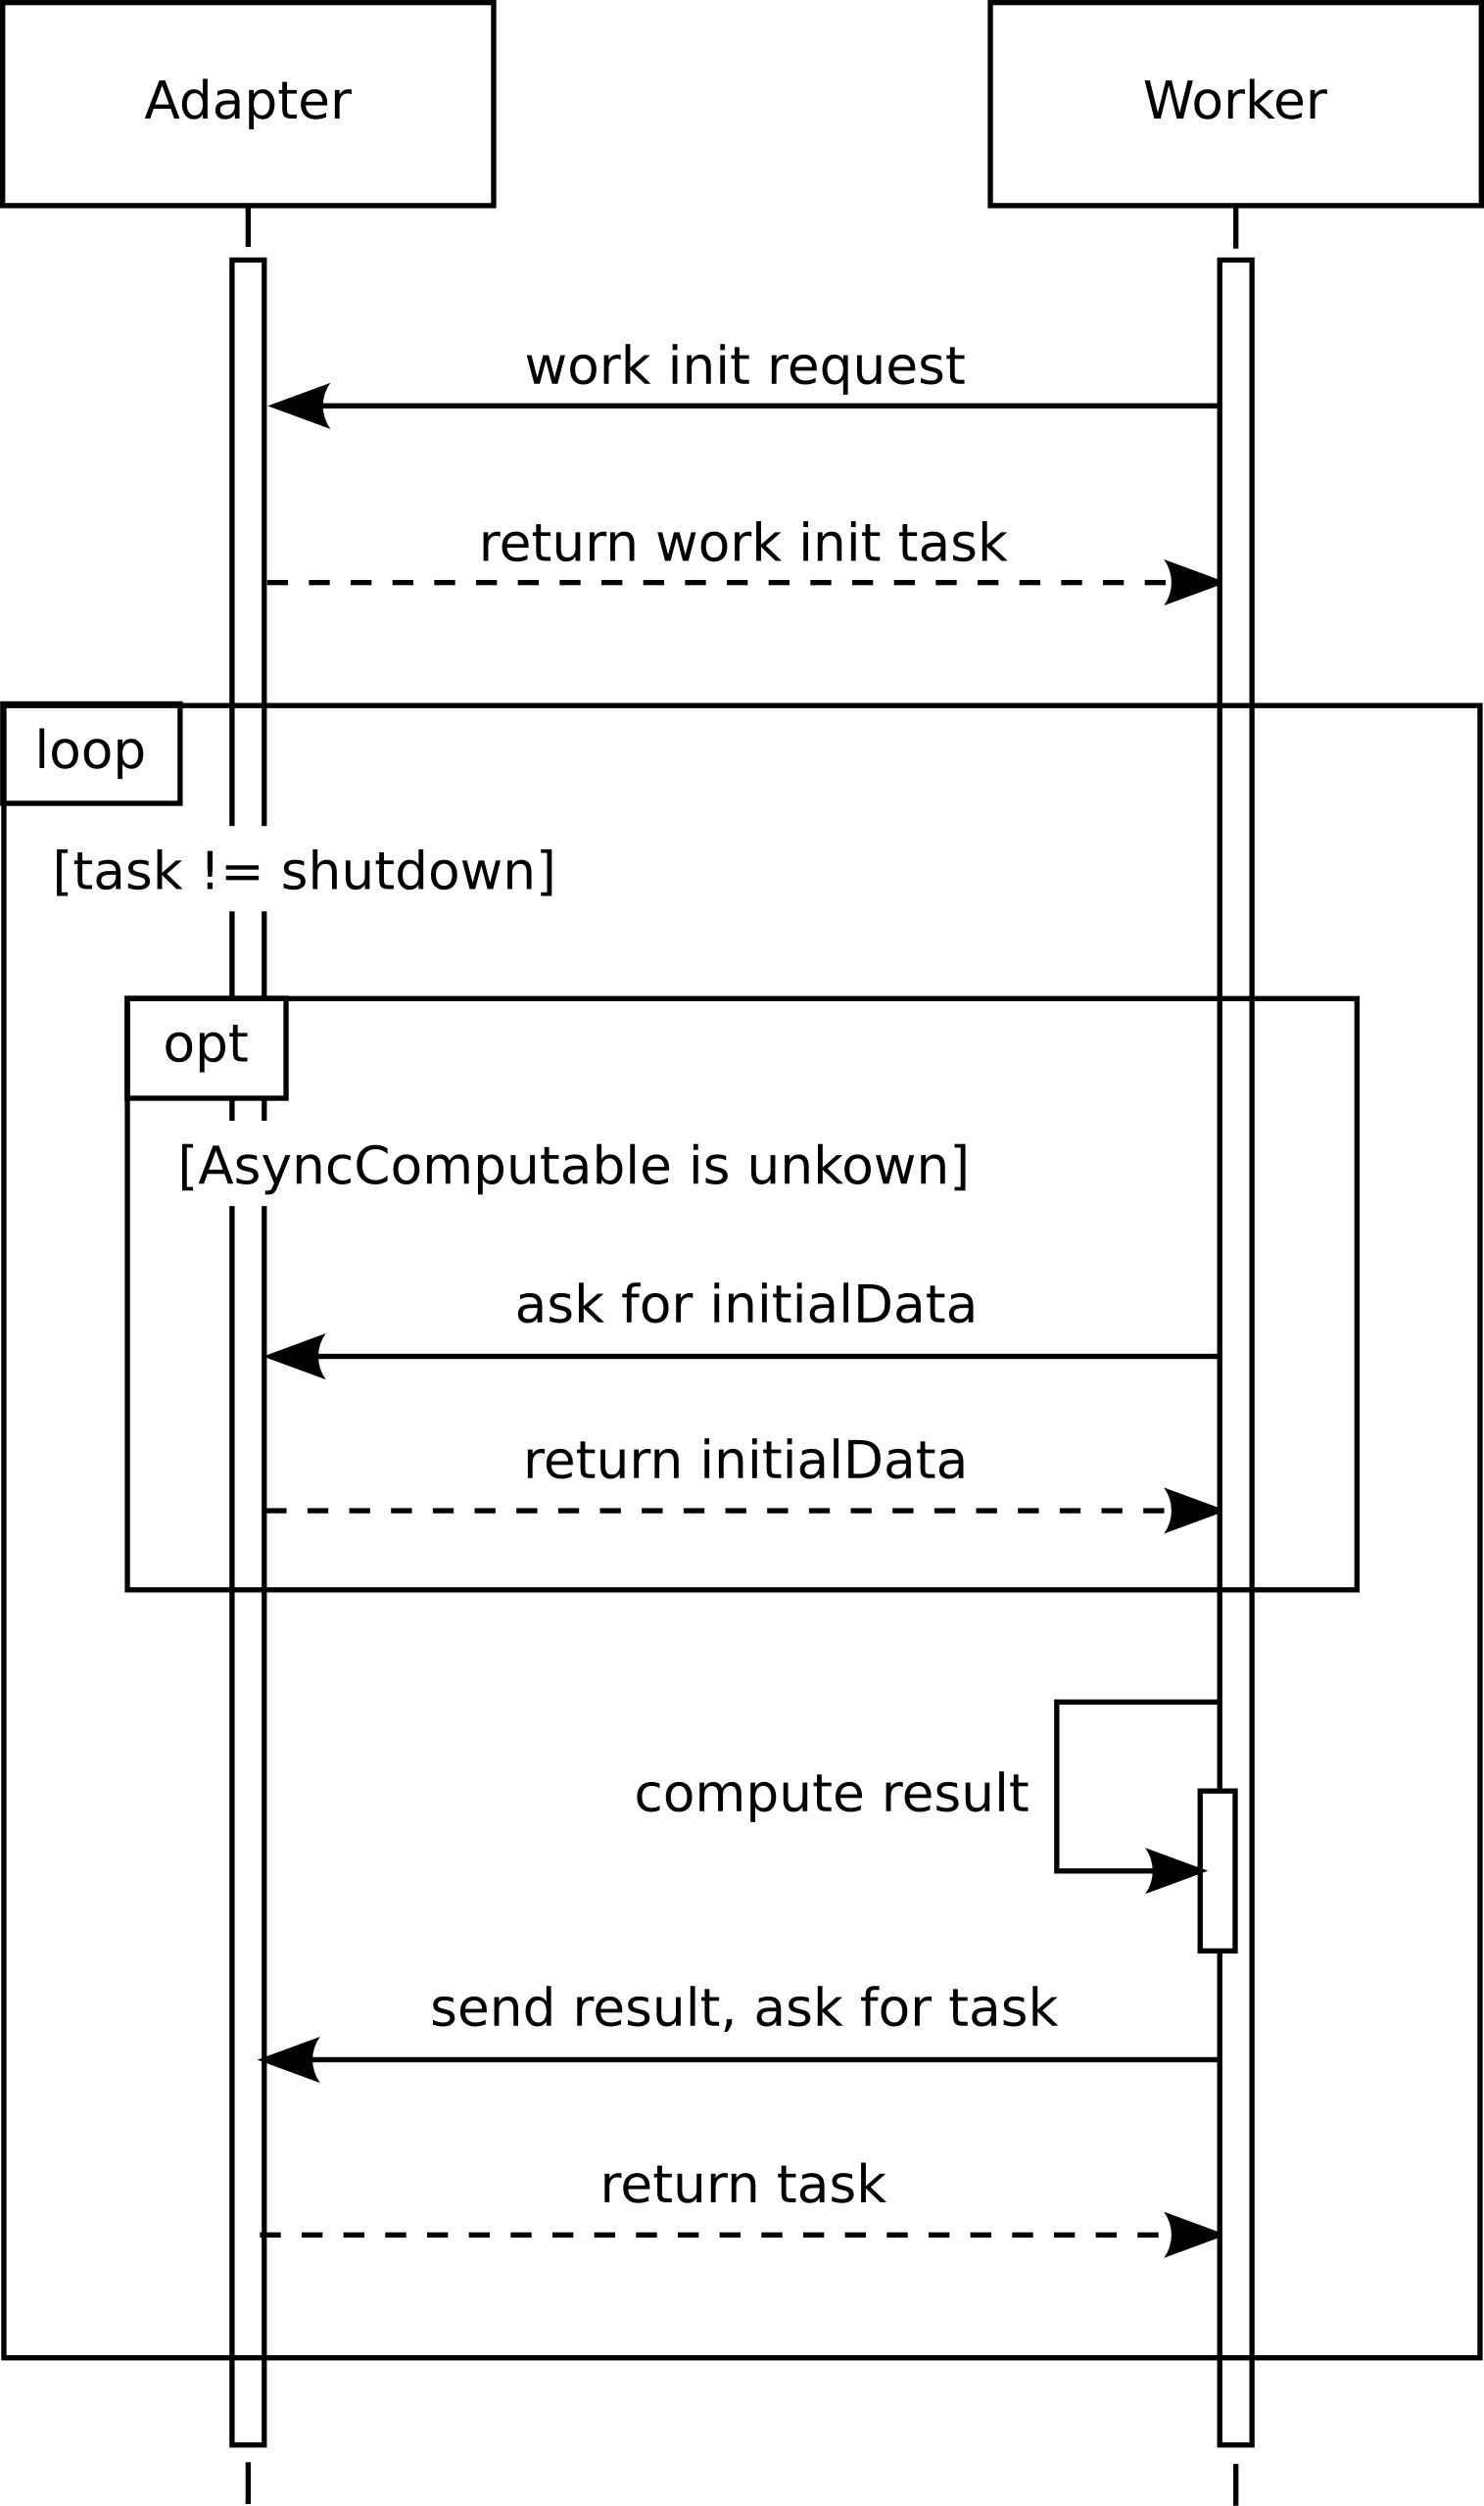
\includegraphics[width=70mm]{communication-flow.png}
  \caption{Communication flow between endpoints and workers}
  \label{fig:communication-flow}
\end{figure}

As one can see in figure \ref{fig:communication-flow}, the communication between endpoints and workers is initialized by the worker. After the worker gets a task from an endpoint, it looks if the needed task configuration is already stored in its internal cache. If the configuration is unknown, the worker requests it from the endpoint. The endpoint responds with the configuration, which is cached by the worker, in case that it is needed again. The worker computes the result for the task using the task data, and the corresponding configuration. The result is then transmitted to the endpoint and a new task is requested.

\section{Enhancements}
\label{chap:impl:enhancements}
Biohadoop provides two enhancements for algorithms, beside the task system presented in section \ref{chap:impl:task-system}. The first one is for persistence, where it is possible to load and store arbitrary data to and from a file system (see section \ref{chap:impl:persistence}). The second enhancement provides high level parallelism between parallel running algorithms, called the ``island model'' (see section \ref{chap:impl:island-model}).

\subsection{Persistence}
\label{chap:impl:persistence}
There are a lot of reasons to store algorithm results to a file system. The most important is to save the final result of a computation. Another reason is to store intermediate results in case something happens. If this data is reloaded afterwards, the computation can continue from that point on. Intermediate results can also be used for other computations or for visualization.

The conclusion is that some kind of persistence is useful. It should include both the saving and loading of data. Biohadoop provides this kind of service by offering a simple API, accessible through the class \texttt{FileUtils}. The API stores provided data in JSON format in a file with a given name. When a file is loaded, the API supposes that the contained data is also in JSON format and tries to deserialize it. An exception is thrown if this is not possible.

The API covers the fundamental persistence use cases, but a programmer is free to use its own mechanism of data storage and retrieval.

\subsection{The island model}
\label{chap:impl:island-model}
The island model is a high level parallelization model that is sometimes used in optimization problems. In the island model, several algorithms run in parallel, trying to compute the result to the same problem. The parallel running algorithms are called the islands. Each of these algorithms is independent of the others, and each one may have a different solution at a given point of time. By exchanging their data after some intervals, islands may get interesting solutions from other islands that can be integrated in their own computation to enhance their solution. If we take the GA as an example, the islands would consist of independently running GAs that exchange individuals to improve the solution. Figure \ref{fig:island-model} shows an example island model with 3 GAs that exchange individuals.

\begin{figure}[ht!]
  \centering
  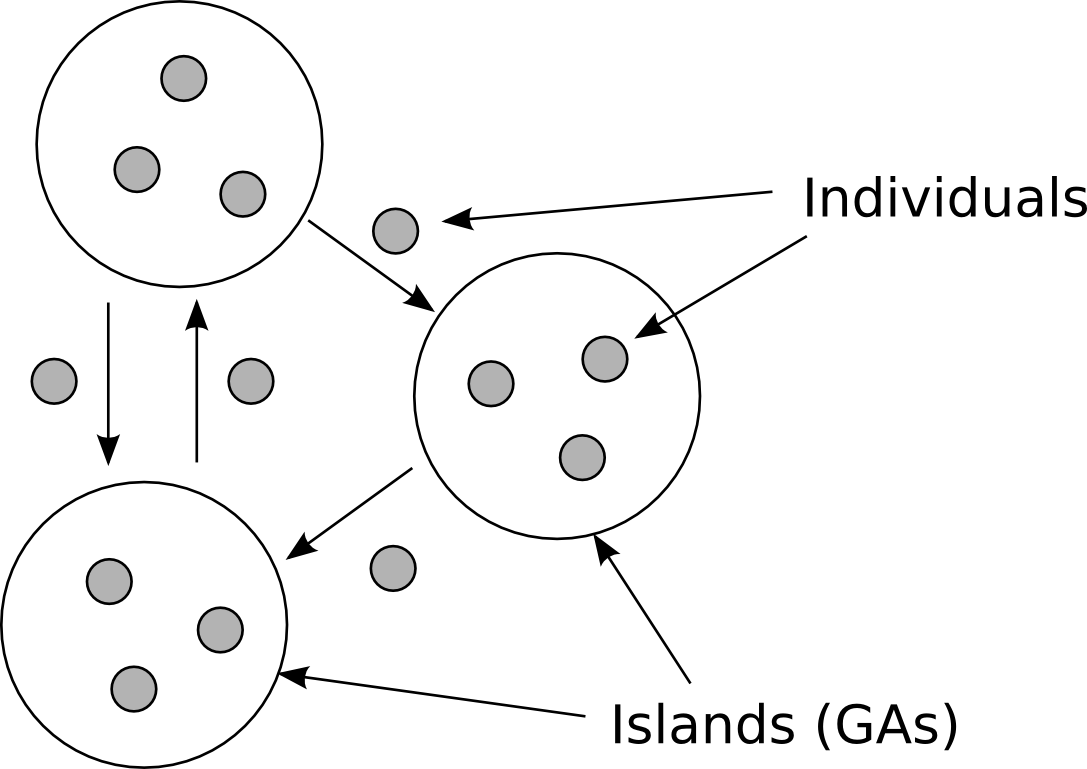
\includegraphics[width=70mm]{island-model.png}
  \caption{Example island model with 3 GAs, exchanging individuals}
  \label{fig:island-model}
\end{figure}

The island model enhances the exploratory behavior of optimization algorithms, which often results in better overall solutions. As the data exchange is only done at certain points of time, the islands have the chance to exploit their own solution. When they get stuck in a local optima, they get the chance to escape this optima by considering solutions from other islands.

Biohadoop provides an API, implemented in the class \texttt{IslandModel}, that can be used to build an island model between any number of algorithms. It provides methods to publish the own solutions to other islands or to merge remote solutions with the own solutions. Data merging can be configured by implementing the interfaces \texttt{RemoteResultGetter} and \texttt{DataMerger}. The \texttt{RemoteResultGetter} defines from which remote island the data should be retrieved. It may take into account different properties, like the number of iterations, the fitness of individuals, etc. The \texttt{DataMerger} defines, how two solutions should be merged.

The island model API uses ZooKeeper \cite{zookeeper}, which is a server that provides distributed configuration and synchronization services and a naming registry. Therefore, a running ZooKeeper instance must be accessible by Biohadoop, if an algorithm wants to use the island model.

By using ZooKeeper as central registry for the island model, it doesn't matter if the algorithms run in the same Biohadoop instance or in different Biohadoop instances. They find each other through their ZooKeeper registrations.

The main advantage of running several algorithms in the same Biohadoop instance is, that it guarantees that they all run at the same time. Scheduling several Biohadoop instances in parallel doesn't guarantee that they also run at the same time, as YARN decides when to launch an application. The island model is useless if the algorithms don't run at the same time.

\section{Configuration}
\label{chap:impl:configuration}
Biohadoop uses a configuration file in JSON format. The advantage of JSON is, that its understandable for humans and usually smaller in size than e.g. XML.

The path to the configuration file must be given on invocation of Biohadoop as its first parameter (more information on how to run Biohadoop can be found in \ref{chap:usage:run}). Biohadoop stops immediately with an exception if the path is empty or wrong or the configuration file can not be parsed.

The configuration file itself consists of the following four top-level objects:
\begin{itemize}
  \item \texttt{communicationConfiguration}: defines a list of endpoints and a list of workers that Biohadoop should start. The worker configuration provides additional information about the number of workers that should be started
  \item \texttt{globalProperties}: a map with strings as keys and values. This properties are used for global settings that should be available in the ApplicationMaster. Examples for such global settings are configurations for Kryo and ZooKeeper.
  \item \texttt{includePaths}: a list of strings that define the paths where needed libraries can be found. This isn't important for a local running instance of Biohadoop (e.g. during development), as the necessary classpaths must be set when starting Biohadoop. But it is important when Biohadoop runs in the Hadoop environment, as this are the paths to libraries that Hadoop should provide to Biohadoop when running. If the paths to the necessary libraries are wrong when running on Hadoop, Biohadoop won't run correctly.
  \item \texttt{algorithmConfigurations}: a list of algorithms that should be run by Biohadoop. Each element in the list describes the configuration for an algorithm. The configured algorithms are started in parallel in the same Biohadoop instance.
\end{itemize}

It is not always convenient to write a configuration by hand, although it is possible. Biohadoop provides two builder classes to make it more easy to produce configuration files. The builder in \texttt{BiohadoopConfiguration} offers methods to configure the top level elements of a configuration file. Algorithm configuration is simplified by the builder in \texttt{AlgorithmConfiguration}. The result of this algorithm configuration can then be handed over to the \texttt{BiohadoopConfiguration} builder.

\section{Biooozie}
\label{chap:impl:oozie}
Biooozie implements a custom action for Apache Oozie (see \ref{chap:hadoop:oozie}) that schedules one or several instances of Biohadoop. The action can be part of a workflow of arbitrary size. The outcome of the custom action is ``ok'' if no error happened during the execution of the action. This is also true for the case that several Biohadoop instances are defined in one action. If any Biohadoop instance fails, the outcome of the action is ``error''.

A short example workflow with three stages copies data sets to a HDFS file system, on which some MapReduce action is performed that produces new data sets. Those data sets in turn are the base for a GA computation, performed by Biohadoop (see figure \ref{fig:biooozie}).

\begin{figure}[ht!]
  \centering
  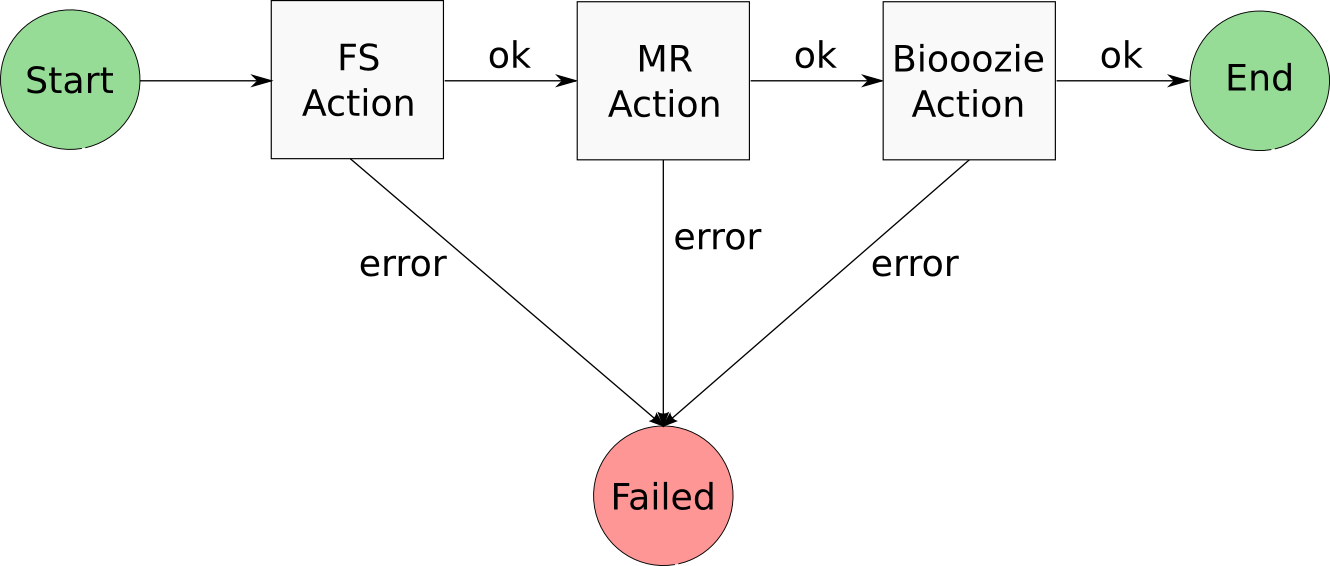
\includegraphics[width=100mm]{biooozie.png}
  \caption{Example Oozie workflow, including Biooozie action}
  \label{fig:biooozie}
\end{figure}

The action is configured in an Oozie workflow as an XML element with name \texttt{biohadoop}. It contains one \texttt{name-node} element that defines the URL of the HDFS NameNode, and one or several \texttt{config-file} elements. Each \texttt{config-file} element represents a Biohadoop instance that starts with the given configuration file. This way it is possible to schedule several Biohadoop instances in parallel, using a single action. The parallel instances are for example useful for running an island model.

The term ``schedule'' is used here on purpose, because Hadoop doesn't guarantee that the instances also run in parallel, this depends on the available Hadoop resources (i.e. on the available YARN containers). It is for example possible that a custom action schedules three instances of Biohadoop, but due to a lack of Hadoop resources, the instances run one after another.

Biohadoop could also be invoked using Oozies \texttt{java} action, the advantage of Biooozie is that its tailored to Biohadoop and there is no need to provide all the parameters that a simple \texttt{java} action needs. 
% DELETABLE!!!!

\chapter{Using Biohadoop}
\label{chap:usage}
One of the design goals of Biohadoop was to provide a framework for distributed computation on the Hadoop platform, that is easy to use. The result is a simple API, that can be used to implement algorithms. This chapter introduces into the necessary steps to write an algorithm that is capable of being run by Biohadoop on a Hadoop environment. In addition, the presented algorithm uses the capabilities of the task system to distribute parts of its work to Biohadoops workers, to achieve a higher level of parallelism.

% \section{Example algorithm}
% \label{chap:usage:algorithm}
% For the sake of simplicity we reuse the example algorithm \texttt{Sum} of chapter \ref{chap:impl:system-architecture}. As mentioned there, it is a simple algorithm, whose only purpose is to sum the values of an integer array. In listing \ref{listing:sum} we have already a first implementation, that is capable of being run by Biohadoop. But in that example, no usage of the task system and therefor distribution is taken. Also, all the parameters are fixed. In the next sections, we will create step by step an implementation that is configurable using Biohadoops configuration file, and that is able to distribute its work (see section \ref{chap:impl:configuration} for more details about the configuration file).
% 
% To make it more transparent how and when we use the task system, we modify the algorithm a little bit. It should use a number of integer arrays (the number is called \texttt{CHUNKS} from here on), each array should be of a fixed size (the size is called \texttt{CHUNK\_SIZE} from here on). If we would append all the chunks one after another, we would have one big integer array of size $\texttt{CHUNCKS} * \texttt{CHUNCK\_SIZE}$. If you look at it from the other side, a big integer array would have to be split into several chunks, to make it suitable for parallel computation. So there is no real difference to the original algorithm, it just preserves us from doing some computations to split a big integer array into smaller arrays. 
% 
% Listing \ref{lst:usage-build-data} shows how the data is created. The method \texttt{buildData(int chunks, int chunkSize)} takes \texttt{CHUNCKS} and \texttt{CHUNCK\_SIZE} as input argument and returns \texttt{CHUNKS} integer arrays, each of size \texttt{CHUNCK\_SIZE}. The arrays are filled with consecutive numbers, starting from 0. The consecutive numbers continue between the boundaries of adjacent arrays. For example, array0=[0,1,2], array1=[3,4,5], ...
% 
% \lstinputlisting[caption=Building the integer arrays for the \texttt{Sum} algorithm,label=lst:usage-build-data]{../listings/chap-usage-buildData.lst}
% 
%   \subsection{Configuring the algorithm}
%   \label{chap:usage:configuration}
%   Lets begin with modifying the algorithm in a way, such that it can be configured by Biohadoops configuration file. The configuration file is read by Biohadoop at its startup, and the private parameters for an algorithm instance are provided when the \texttt{compute(SolverId solverId, Map<String, String> properties)} method of the algorithm is called. If we use the configuration file of listing \ref{lst:sum-configuration}, we see that we get two properties:
%   \begin{itemize}
%     \item \texttt{CHUNKS}: the number of integer arrays, that should be produced by the algorithm.
%     \item \texttt{CHUNK\_SIZE}: the size of each integer array.
%   \end{itemize}
%   Those parameters are of type \texttt{String}, so we need to convert them first to integer values, to make them suitable for the \texttt{buildData(int, int)} method, mentioned in listing \ref{lst:usage-build-data}. After this steps are taken, we have configured our algorithm through a Biohadoop configuration file, and we have initialized the data. Listing \ref{lst:usage-configured} shows, how the algorithm looks at the current stage. The \texttt{buildData(int, int)} method was skipped, to make the code more concise, it can be found in listing \ref{lst:usage-build-data}.
%   
%   \lstinputlisting[caption=Configuring the \texttt{Sum} algorithm and initializing the data,label=lst:usage-configured]{../listings/chap-usage-configured.lst}
% 
%   \subsection{Parallelization using the task system}
%   \label{chap:usage:parallel-algorithm}
%   The parallelization of an algorithm using Biohadoop consists of four steps:
%   \begin{enumerate}
%     \item provide an implementation of \texttt{AsyncComputable}, that can be used to compute the task results by the workers.
%     \item create a task submitter, that can be used to add new tasks to the task system.
%     \item submit tasks to the task system, by using the before mentioned submitter.
%     \item wait for the tasks to complete. It is possible to block during the wait process, but is also possible to do other work in between.
%   \end{enumerate}
%   
%   In step 1 we have to implement \texttt{AsyncComputable}. The resulting class can be used by the workers to compute the results for the tasks. In our case, the workers get as input arguments an integer array and have to compute the sum over all of its elements. Listing \ref{lst:usage-async-computable} shows how this would be done in a class with name \texttt{AsyncSumComputation}. We see that this class is typed, the types have to match the task submitter in step 2. The types are \texttt{Object} for the \texttt{initialData}, but we don't take usage of it in this case. The input data is of type \texttt{int[]}, which matches our integer arrays. As output we have a single integer, which is the result of the summation. The content of the method itself is straight forward.
%   
%   \lstinputlisting[caption=Summation of all values in an integer array\, done in an \texttt{AsyncComputable} class\, that is suitable to be run by workers,label=lst:usage-async-computable]{../listings/chap-usage-asyncComputable.lst}
%   
%   Step 2 demands the creation of a task submitter, to be able to add tasks to the task system. Lets clarify at this point, what a single task means in our example program: each single task consists of computing the sum of an integer array. The data for this task is the given integer array. This data is send to workers, that use a given \texttt{AsynComputable} class to compute the result - in our case the sum of the integer array computed by the \texttt{AsyncSumComputation} class. The result is then returned to the algorithm, at which point the task has completed.
%   
%   The \texttt{Sum} example algorithm uses many integer arrays, therefor we have many tasks, one task for every integer array. Tasks are submitted to the task system, by submitting their data through a task submitter. The usage of a task submitter is advised, as it hides some complexity from the algorithm author. But it is possible to communicate to the task system without a submitter. We choose to use the task submitter, and create a new one the following way:
%   
%   \begin{lstlisting}
% TaskSubmitter<int[], Integer> taskSubmitter = new SimpleTaskSubmitter<Object, int[], Integer>(AsyncSumComputation.class);
%   \end{lstlisting}
%   
%   This task submitter is configured to get an object of type \texttt{Object} as \texttt{initialData}. As we don't want to use this feature, we don't provide such an \texttt{initialData}. The submitter is further configured to receive tasks of type \texttt{int[]} and to return \texttt{TaskFutures} of type {Integer}, that can be used by the algorithm to retrieve the results from the task system. The tasks of type \texttt{int[]} that we are going to submit are exactly the arrays, that we created in the previous section, using the \texttt{buildData(int, int)}. We store all those arrays in a single 2-dimensional array of type \texttt{int[][]} and call this array \texttt{data}. The only parameter that we provide to the new instance of \texttt{SimpleTaskSubmitter} is the \texttt{AsyncSumComputation} class. This class is used by the workers to compute the results for the tasks, that are submitted through this task submitter.
% 
%   In step 3 we start to submit tasks to the task system. As we want to submit a number of arrays, it is best to do it in a loop. We also want to be able to use the results of the different sums to compute the final sum. Therefor we have to store the \texttt{TaskFutures}, to be able to retrieve their results:
%   
%   \begin{lstlisting}
% List<TaskFuture<Integer>> taskFutures = new ArrayList<>();
% for (int i = 0; i < chunks; i++) {
%   TaskFuture<Integer> future = taskSubmitter.add(data[i]);
%   taskFutures.add(future);
% }
%   \end{lstlisting}
%   
%   Step 4 consists of waiting for the results. The \texttt{get()} method of a \texttt{TaskFuture} provides us the result, but blocks until a result is available. \texttt{TaskFuture} provides also a \texttt{isDone()} method, which we can use to check for finished computations in a non-blocking way. If \texttt{isDone()} returns true, we can get the results by invoking \texttt{get()}, that doesn't block anymore at that time.
%   
%   We choose the simpler \texttt{get()} approach at the cost of blocking the algorithm. As we need all results to proceed, this makes no difference to the non-blocking variant. Because we got several \texttt{TaskFuture} objects from our task submissions in step 3, we have to loop on all the \texttt{TaskFuture} objects to get all of their results. By summing up the results, we get the final sum over all arrays:
%   
%   \begin{lstlisting}
% int sum = 0;
% for (TaskFuture<Integer> future : taskFutures) {
%   sum += future.get();
% }
%   \end{lstlisting}
%   
%   After this step completes, we have the final sum over all arrays, and the algorithm can terminate.
%   
%   Something that wasn't mentioned until now is, that the task submission and result retrieval operations may throw checked exceptions. This exceptions must be caught, therefor the submission and retrieval must be surrounded by a \texttt{try ... catch} block. In the example code above, this step was omitted to keep the code clear and concise. In the appendix, the whole code can be found, once for the \texttt{Algorithm} (see listing \ref{lst:appendix-sum-full}), and once for the \texttt{AsyncComputable} (see listing \ref{lst:appendix-sum-async}). More examples can be found at \cite{biohadoop-algorithms}.
  
\section{Run Biohadoop}
\label{chap:usage:run}
Although the main purpose of Biohadoop is to be run in a Hadoop environment, it can also be run in a local environment. This is for example useful when new algorithms are developed. In this case, the whole process of compilation, deployment to a Hadoop environment and testing can be abbreviated.

To run Biohadoop, three components must be available (four if Biohadoop is started in a Hadoop environment):

\begin{itemize}
  \item An installation of Java in version 1.7 or higher. From here on it is assumed, that Java is installed and configured and that the \texttt{JAVA\_HOME} variable points to this installation.
  \item All necessary libraries must be present and accessible in one or several folders.
  \item A valid configuration file must be present and accessible.
  \item The fourth component is only necessary when running Biohadoop in a Hadoop environment. This component is Hadoop itself, which must be available in a version $\geq 2$.
\end{itemize}

If those three components are provided (four for running on Hadoop), Biohadoop can be started. In a local environment, this is done by setting the right class paths when launching the program. In a Hadoop environment, the configuration option \texttt{includePaths} must be set, to include the necessary files (see \ref{chap:impl:configuration} on more information about configuring Biohadoop). Those paths have to point to valid locations of an accessible HDFS file system.

Biohadoop was developed using Maven. \footnote{\url{http://maven.apache.org/} last access: 11.09.2014} Therefor it is rather easy to get all the needed libraries, as they are declared as dependencies. The source code for Biohadoop can be found at \cite{biohadoop}. By invoking the following command on the projects root folder, all dependencies are accumulated and put to the sub folder \texttt{target/dependency}:

\begin{lstlisting}[language=bash]
mvn dependency:copy-dependencies
\end{lstlisting}

From there, they can be directly referenced through Javas \texttt{classpath} option when running in a local environment. When running in a Hadoop environment, the libraries need to be copied to an accessible HDFS file system, and this location must be present in the before mentioned \texttt{includePaths} configuration option.

For a quick tutorial on how to compile and run Biohadoop from the sources, please refer to appendix \ref{chap:appendix:biohadoop-quickstart}. To use Biohadoop in a Hadoop environment, such an environment must be present. It can be a difficult task to configure such a Hadoop environment, therefor in appendix \ref{chap:appendix:biohadoop-docker} a simple method can be found, to use a pre-build Hadoop environment. The only dependency this environment has, is Docker \cite{docker}, which is a simple and lightweight runtime for containers, available on all major operating systems.

\subsection{Local environment}
\label{chap:usage:local}
To start Biohadoop in a local environment, the class paths need to be set to include the necessary libraries. The necessary libraries can be obtained by invoking the Maven command, outlined above. As an additional parameter, the \texttt{-Dlocal} option must be provided to Java. This is the only way to tell Biohadoop that it is launched in a local environment. If this parameter is missing, Biohadoop will complain that it can't connect to Hadoop.

Lets assume, that all of the necessary libraries can be found at the location \path{/home/user/biohadoop/libs}, and the configuration file can be found at \path{/home/user/biohadoop/configs/simple-config-json}. Then, Biohadoop can be started in local mode by running the following command:

\begin{lstlisting}[language=bash]
java -Dlocal -cp /home/user/biohadoop/libs/* at.ac.uibk.dps.biohadoop.hadoop.BiohadoopApplicationMaster /home/user/biohadoop/configs/simple-config-json
\end{lstlisting}

A little bit hidden in the command we find the main class that starts Biohadoop, \texttt{at.ac.uibk.dps.biohadoop.hadoop.BiohadoopApplicationMaster}. This class takes care of starting the configured algorithms, adapters and workers. After all of the algorithms have terminated, either because they have finished their computation or because they had errors, Biohadoop shuts down.

When running Biohadoop in the local environment, all workers are started as threads in the same JVM as Biohadoop (in contrast to a Hadoop environment, where the workers are started in separate JVMs on perhaps different machines). This leads to the fact, that the workers have full access to all (static) objects of Biohadoop, for example the \texttt{Environment} object (see \ref{chap:impl:configuration} for a description of this object). But when those workers are started in a Hadoop environment, this access is not given anymore. So, one has to take care to rely only on the objects and properties, that are provided to the used methods.

\subsection{Hadoop environment}
\label{chap:usage:hadoop}
To start Biohadoop in a Hadoop environment (for example in the one provided in appendix \ref{chap:appendix:biohadoop-docker}), all needed libraries and configuration files must be present in the HDFS file system. In addition, Biohadoops jar file must be accessible through the local file system, as it is started directly by Hadoop. The location of the libraries and configuration files in the HDFS file system must be configured in the configuration file, that is provided to Biohadoop on startup.

Lets assume, that all of the necessary libraries can be found at the HDFS location \path{/biohadoop/libs}, the configuration file can be found at the HDFS location \path{/biohadoop/configs/simple-config-json} and that those paths are part of the configuration file that is provided to Biohadoop at startup. Further more, Biohadoops jar file can be found at \path{/home/user/biohadoop/biohadoop.jar}. Then, Biohadoop can be started in Hadoop mode by running the following command:

\begin{lstlisting}[language=bash]
yarn jar /home/user/biohadoop/biohadoop.jar at.ac.uibk.dps.biohadoop.hadoop.BiohadoopClient /biohadoop/configs/simple-config-json
\end{lstlisting}

As one can see, now the command \texttt{yarn} is used to launch Biohadoop. This command takes care of setting all the needed Hadoop environment variables, after which it starts the provided main class. The \texttt{yarn} command is part of Hadoop since version 2, and should be available if Hadoop is configured in the right way. If it is not available, please contact the system administrator.

In contrast to running Biohadoop in local mode, we have now a different main class, that is launched. This is due to the fact, that Yarn needs a startup class, from where it loads the main program. By looking at the source code of \texttt{at.ac.uibk.dps.biohadoop.hadoop.BiohadoopClient}, one will notice that it starts the \texttt{BiohadoopApplicationMaster} behind the curtains (\texttt{BiohadoopApplicationMaster} is the class that is directly started in local mode).

When running Biohadoop in a Hadoop environment, all workers are started in their own containers, which are under the control of Hadoop. The result is, that the workers can not access the (static) objects of Biohadoop, if one wants to access some properties of Biohadoop, this must be done through the provided communication facilities of Biohadoop. It is nevertheless possible to implement some different communication facilities, if this is needed.
% \chapter{Evaluation}
\label{chap:evaluation}
Biohadoops purpose is to facilitate the implementation of parallel algorithms on Hadoop. It is expected that the execution time of an algorithm reduces if it is parallelized (assuming the algorithm is suitable for parallelization). As this cannot be guaranteed without proper measurement, this chapter is devoted to the study of Biohadoops speedup characteristics.

Two bio-inspired optimization algorithms are used as benchmarks. Both use Biohadoop and its task system to solve a test problem. The algorithms and test problems are described in section \ref{chap:evaluation:testproblems}.

The algorithms are executed on a Hadoop cluster to study the impact on their execution times by varying problem sizes and number of workers. Benchmark details can be found in section \ref{chap:evaluation:benchmarks}. Results are presented in section \ref{chap:evaluation:benchmarks}.

\section{Hardware}
All experiments were performed on a Hadoop cluster with 6 identical computers. Each machine has the following specifications:

\begin{itemize}
  \item Intel Core2 Duo CPU E8200 @ \unit[2.66]{GHz} (2$\times$\unit[2.66]{GHz}, no hyperthreading)
  \item \unit[6]{MB} shared L2 cache, \unit[32]{KB} L1 data cache, \unit[32]{KB} L1 instruction cache
  \item \unit[4]{GB} (2$\times$\unit[2]{GB}) DDR2 RAM @ \unit[667]{MHz}
\end{itemize}

The computers are directly connected to the same Switch through a 1Gb (Gigabit) Ethernet network.

\section{Test Problems}
\label{chap:evaluation:testproblems}
Both implemented algorithms are part of the GA family. They differ in the number of objectives that they can handle. While NSGA-II is used to solve the MOP in section \ref{chap:evaluation:zdt3}, a simple GA is used to solve the SOP in section \ref{chap:evaluation:tiledmul}.

\subsection{ZDT-3}
\label{chap:evaluation:zdt3}
The first optimization algorithm is NSGA-II that is used to find optimal solutions for the Zitzler–Deb–Thiele's function nr. 3 \cite{zitzler2000comparison}. ZDT-3 is a well known MOP and therefore suited as a test problem. The task is to find an approximation to the optimal Pareto Front, given in figure \ref{fig:zdt3}.

\begin{figure}
  \centering
  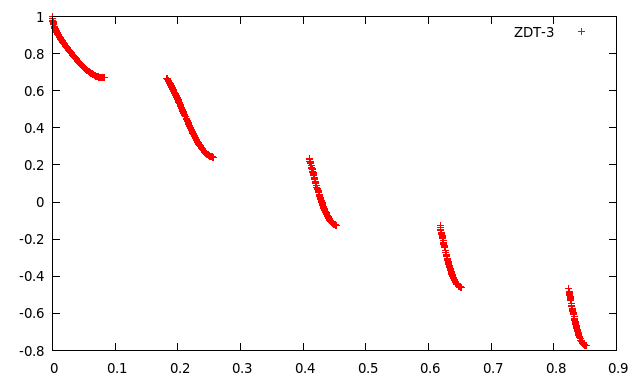
\includegraphics[width=110mm,natwidth=640,natheight=384]{zdt3.png}
  \caption[Optimal Pareto Front for ZDT-3]{Optimal Pareto Front for ZDT-3}
  \label{fig:zdt3}
\end{figure}

The implementation uses Biohadoop workers to create and evaluate the offsprings. Simulated Binary Crossover (SBX) and Parameter based mutation \cite{deb2000efficient} are used for the offspring creation. The fitness is computed using the ZDT-3 function. The selection of the fittest individuals for the next population is based on ranking and crowding distance and is performed on the master.

\subsection{Tiled Matrix Multiplication}
\label{chap:evaluation:tiledmul}
The second benchmark implements a GA to solve the SOP for finding optimal tile sizes for the tiled matrix multiplication (TMM). The objective is to minimize the execution time for a matrix multiplication.

A matrix multiplication can be performed in different ways. The most obvious one is the standard algorithm:
\begin{lstlisting}
for i = 1 to n
  for j = 1 to m
    for k = 1 to l
      C(i,j) = C(i,j) + A(i,k) * B(k,j)
\end{lstlisting}

The matrix multiplication can be improved by loop tiling \cite{wolfe1989more}. The computation is performed on smaller blocks (tiles) of the matrices:
\begin{lstlisting}
for i0 = 1 to n, step blocksize_i
  for j0 = 1 to m, step blocksize_j
    for k0 = 1 to l, step blocksize_k
      for i = i0 to min(i0 + blocksize_i, n)
        for j = j0 to min(j0 + blocksize_j, m)
          for k = k0 to min(k0 + blocksize_k, l)
            C(i,j) = C(i,j) + A(i,k) * B(k,j)
\end{lstlisting}

If the blocks are small enough they fit into the L1 CPU cache which results in a speedup. For example, the average of ten consecutive test multiplications of two matrices of size 1024$\times$1024 took 11.384 seconds for the simple matrix multiplication and 2.669 seconds for the tiled multiplication with tile sizes $i=32$, $j=32$ and $k=32$, using a single computer of the test system mentioned above. This numbers show that it is appropriate to use the tiled approach for the matrix multiplication. But the speed of TMM depends heavily on the tile sizes, the same tiled multiplication as above with tile sizes of $i=1$, $j=1$ and $k=1$ took 25.683 seconds to finish, an increase of about than 10 times compared to a good tile size. Because of the number of possible tile size combinations and the time it takes to execute a matrix multiplication (e.g. matrix size=1024, 2 seconds for a matrix multiplication: $1024^3 \times 2 = 2\times{10^9} $ seconds), it is not feasible to do an exhaustive search for the optimal tile sizes.

An optimization algorithm can be used to find the (near) optimal tile sizes for the different loops. In this case, the optimization is done using a GA. The implementation uses Biohadoops workers to create and evaluate an offspring. For the offspring creation, Simulated Binary Crossover (SBX) and Parameter based mutation are used. The fitness is computed as the time it takes to multiply two matrices using a given tile size. The selection of the fittest individuals for the next population is performed on the master.

\section{Benchmarks}
\label{chap:evaluation:benchmarks}
The task of the benchmarks is to find the speedup characteristics of Biohadoop. The assumption is that the execution time of an algorithm depends both on the problem size and the number of workers. To evaluate this assumption, the algorithms presented in section \ref{chap:evaluation:testproblems} are executed with different problem sizes and different numbers of workers. The execution times are measured and used to calculate the speedup using the formula $S = T_S / T_P$, where $S$ is the speedup, $T_S$ is the time for a serial execution and $T_P$ is the time for parallel execution. The results are discussed in section \ref{chap:evaluation:result}.

%  Amdahl's law \cite{amdahl1967validity}

A benchmark is defined by a given algorithm (e.g. NSGA-II) and its settings (e.g. number of workers, number of iterations, etc.). All performed benchmarks have the following settings in common:
\begin{itemize}
  \item The number of iterations is set to 250.
  \item The population size is set to 100.
  \item The distribution index $n_c$ for the SBX crossover is set to 20.
  \item The distribution index $n_m$ for the mutation is set to 20.
  \item The mutation probability for each offspring value is set to $1/n$, i.e., on average one offspring value is mutated.
\end{itemize}

The test problems have also exclusive settings that only apply to them. For ZDT-3 this is the genome size. The genome size corresponds to the number of values of an individual and the dimension of the solution space. Each individual is represented by its genome. ZDT-3 can handle any genome size. Changing this number influences two properties of the ZDT-3 benchmark. First, increasing the number of genomes also increases the computation effort for the workers that generate new offsprings and compute their fitness. This is due to the fact that workers generate new individuals using parent genomes and that the ZDT-3 algorithm, used for the fitness computation, loops over all genomes. Second, the genome size influences the amount of data that has to be transferred between the master and the workers. Each worker repeatedly receives two parent individuals and returns an offspring and its computed fitness. The amount of data send between master and workers is, therefore, related to the gnome size of each individual.

The exclusive setting of TMM is the matrix size. It influences the number of computations that need to be performed for a full matrix multiplication and, therefore, also influences the execution time. In contrast to the first problem, the matrix size has no impact on the amount of data transferred between the master and the workers. The matrices are part of the ``initial data'' (see chapter \ref{chap:impl:worker}) and, hence, transferred exactly once to every worker. The task data consists of two parent individuals that are transferred from the master to the workers to create a new offspring and compute its fitness. The data transferred from a worker to the master contains the offspring and its computed fitness value. Each individual consists of its tile sizes for $i$, $j$ and $k$.

The genome size for different ZDT-3 benchmarks is set to 10, 100, 1000 and 10000. The matrix size for TMM is set to 128$\times$128 and 256$\times$256. The execution time for each setting is measured for a number of workers that range from 1 to 15. Each benchmarks is repeated five times to improve the reliability of the results, making it 300 benchmark runs for ZDT-3 (4 genome sizes $\times$ 15 worker setting $\times$ 5 repetitions) and 150 benchmark runs for TMM (2 tile sizes $\times$ 15 worker settings $\times$ 5 repetitions).

\section{Results}
\label{chap:evaluation:result}
The execution time of a Biohadoop application is composed of the time Biohadoop needs to start up and the algorithm execution time. The start up begins with Biohadoops submission to Hadoop and ends when the algorithms \texttt{run} method is invoked. The algorithm execution time starts with the invocation of the algorithms \texttt{run} method and ends when this method returns.

The distinction between start up time and algorithm execution time is made because the main part of the start up time is spent between the application submission to YARN and the beginning of its execution. It is not possible to predict when an application is executed by Hadoop, it depends on different factors like the available cluster resources. To minimize the impact of this uncertainty, the following measurements are based on the algorithm execution time, without the application start up time. The start up time over all benchmarks range from \unit[2.378]{s} to \unit[6.147]{s}, with a median of \unit[3.864]{s}, a \unit[25]{\%} quartile of \unit[3.145]{s} and a \unit[75]{\%} quartile of \unit[4.258]{s}. The mean value is \unit[3.781]{s}. These start up times are close to each other, because the used cluster was completely dedicated to the benchmarks. The start up may take longer when the cluster usage is higher.

Table \ref{table:theoretical_speedup} gives an impression how well the benchmark problems are suited to parallelization by showing the maximum theoretical speedup. The theoretical speedup was calculated using the formula $S = T / (T - t_p)$ from Amdahl's law \cite{amdahl1967validity}, where $S$ is the speedup, $T$ the algorithm execution time and $t_p$ is the time spent in code parts that are parallelized using Biohadoops task system. $T$ and $t_p$ were taken from the average benchmark times with one worker.

\begin{table}
  \centering
  \caption{Theoretical speedups}
  \begin{tabular}{lr}\toprule[2pt]
    Test Problem & Theoretical Speedup \\ \midrule
    NSGA-II, 10 genomes & 7.028 \\
    NSGA-II, 100 genomes & 7.600 \\
    NSGA-II, 1000 genomes & 12.008 \\
    NSGA-II, 10000 genomes & 11.124 \\
    128$\times$128 tiled mul & 81.359 \\
    256$\times$256 tiled mul & 212.169 \\ \bottomrule[2pt]
  \end{tabular}
  \label{table:theoretical_speedup}
\end{table}

% One can see from the theoretical speedups that ZDT-3 is not well suited for parallelization. This is due to the fact that the fitness evaluation is not compute intense. Its time consuming part is a sum over the genomes of an individual, implemented as loop. For example, in the case of 10 genomes per individual this loop would be repeated 10 times. Bigger genome sizes mitigate this effect but have the drawback that the communication time between the master and the workers increases, which negatively affects the speedup. TMMs on the other side show a big potential for parallelization.

The algorithm execution time results for the benchmarks can be found in the boxplots in figures \ref{fig:nsga_250_100_10}, to \ref{fig:nsga_250_100_10000} for the ZDT-3 benchmarks and in figures \ref{fig:tiledmul_250_100_128x128} and \ref{fig:tiledmul_250_100_256x256} for the TMM. The number of workers and the algorithm execution time is plotted on the x-axis and y-axis, respectively.

\subsection{Influence of YARN Container Placement}
The first thing to note when looking at the figures is that the five benchmark times for a given setting (e.g. NSGA-II, 10 genomes) and one worker are very different. The explanation for this effect can be found in the YARN container placement. If a worker container is executed on the same machine as the master container, they communicate without using the physical network. This effect brings a huge performance gain, as can be seen for example in figure \ref{fig:nsga_250_100_100}. In the single worker benchmarks, 4 out of 5 benchmarks executed with both the master and worker container running on the same machine. The result was a \unit[50]{\%} better performance (\unit[9.761]{s} average) compared to the fifth benchmark (\unit[14.164]{s}) where the master and worker were executed on different machines.

% This explanation also applies to the single worker ZDT-3 benchmarks with 1000 (figure \ref{fig:nsga_250_100_1000}) and 10000 (figure \ref{fig:nsga_250_100_10000}) genomes and the single worker TMM with 256 elements (figure \ref{fig:tiledmul_250_100_256x256}). The TMM for one worker and 128 elements (figure \ref{fig:tiledmul_250_100_128x128}) shows the results when the containers of all of the five benchmarks run on different machines. The explanation for ZDT-3 with one worker and 10 genomes (figure \ref{fig:nsga_250_100_10}) is a little bit different. The containers on all five benchmarks run on different machines, nonetheless Hadoop delayed the start of the worker container for two benchmarks by about 2s. The underlying reasons are unknown.

The number of worker containers running on the same machine as the master can also have a negative effect on the execution times. This is especially true if the master is already at the limit of the machines resources and must share them with the workers. An example for this can be found in figure \ref{fig:nsga_250_100_10} for 8 workers. Two worker containers were executed on the same machine as the master during 2 out of 5 benchmarks. The execution time results were \unit[87.977]{s} and \unit[88.014]{s}. In the remaining 3 benchmarks, only one worker container was executed on the same machine as the master, leaving more resources to the master. This results in execution times of \unit[68.423]{s} on average, a difference of more than \unit[20]{\%}.

Therefore, it depends on the available resources of a machine if the execution of worker containers on the same machine as the master container provides benefits or drawbacks. If a resource like CPU or network is already at its limit, additional worker containers slow the whole Biohadoop execution down. If there are enough resources available, the execution of worker containers on the same machine as the master provides benefits, as the communication between the master and the workers can be performed without network usage.

The location of the YARN containers can currently not be influenced, but discussions by the YARN developers suggest that future versions of YARN will support this feature.

% Figure \ref{fig:nsga_250_100_100} is used as example: for the setting with one worker, 4 out of 5 benchmarks executed with both the master and worker container running on the same machine, resulting in a 50\% better performance. A worker that is located on the same machine as the master can communicate to the master without using a physical network, which reduces the communication time. During the fifth benchmark, the master and worker were executed on different containers. The 4 benchmarks with master and worker on the same machine took 9,761s on average, the benchmark where master and worker were located on different machines took 14.164s to execute. This explanation also applies to the single worker ZDT-3 benchmark with 1000 and 10000 genomes and the single worker TMM with 256 elements. The TMM for one worker and 128 elements shows how the result looks like if the containers always run on different machines. The explanation for ZDT-3 with one worker and 10 genomes is a little bit different: the start of the worker containers is delayed by about 2s, only after this time the algorithm can make progress. Hadoop is responsible for this delay, the underlying reasons are unknown.

\subsection{ZDT-3}
\label{chap:evaluation:result:zdt3}
The next thing to notice are the speedups for the ZDT-3 benchmarks. ZDT-3 is not well suited for parallelization as can be seen from the theoretical speedups in table \ref{table:theoretical_speedup}, but the results are even worse than expected, with maximum speedups of 1.619 for 10 genomes, 1.513 for 100 genomes, 2.498 for 1000 and 2.479 for 10000 genomes. Figure \ref{fig:speedup} shows the speedup results of the ZDT-3 benchmarks together with the speedups for TMM.

\begin{figure}
  \centering
  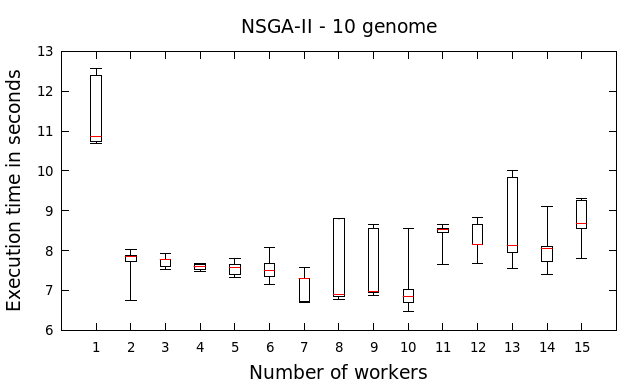
\includegraphics[width=100mm,natwidth=640,natheight=384]{nsgaii_250_100_10.png}
  \caption[ZDT-3 execution times for a genome size of 10]{ZDT-3 execution times for a genome size of 10}
  \label{fig:nsga_250_100_10}
\end{figure}
\begin{figure}
  \centering
  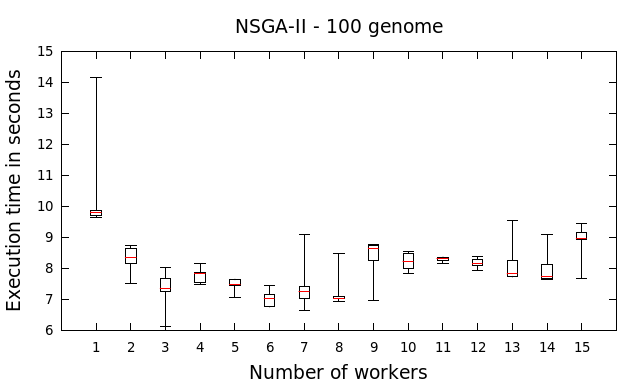
\includegraphics[width=100mm,natwidth=640,natheight=384]{nsgaii_250_100_100.png}
  \caption[ZDT-3 execution times for a genome size of 100]{ZDT-3 execution times for a genome size of 100}
  \label{fig:nsga_250_100_100}
\end{figure}
\begin{figure}
  \centering
  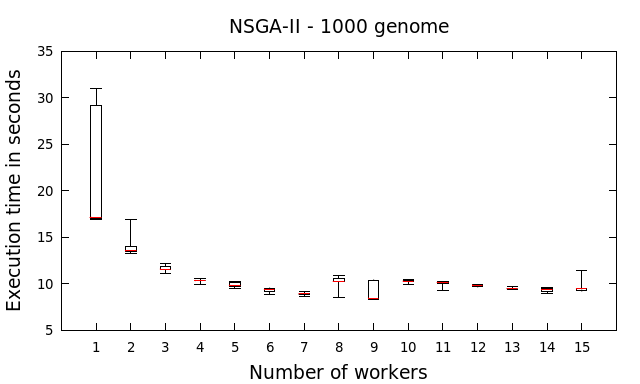
\includegraphics[width=100mm,natwidth=640,natheight=384]{nsgaii_250_100_1000.png}
  \caption[ZDT-3 execution times for a genome size of 1000]{ZDT-3 execution times for a genome size of 1000}
  \label{fig:nsga_250_100_1000}
\end{figure}
\begin{figure}
  \centering
  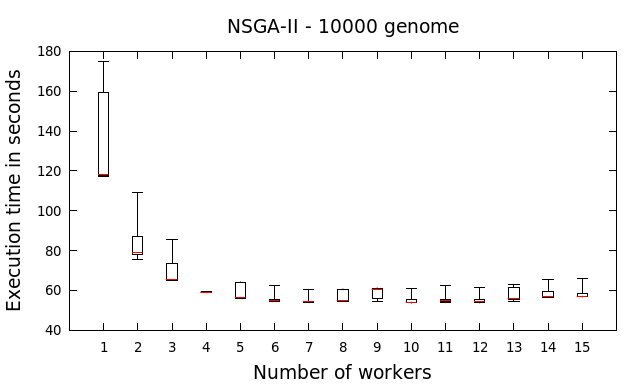
\includegraphics[width=100mm,natwidth=640,natheight=384]{nsgaii_250_100_10000.png}
  \caption[ZDT-3 execution times for a genome size of 10000]{ZDT-3 execution times for a genome size of 10000}
  \label{fig:nsga_250_100_10000}
\end{figure}

The ZDT-3 benchmarks seem to suffer from the lack of one or more resources (bound by the resources), which prohibits further speedup increases. The investigations show that the ZDT-3 benchmarks are not bound by memory, i.e., memory issues don't slow the execution down. All benchmarks start with \unit[256]{MB} of Java heap memory, which is enough for the containers to execute without causing excessive garbage collections. This was established by using the tool jvisualvm (delivered with Java) for the ZDT-3 benchmark with 10000 genomes. The memory usage for the master container is at about \unit[100]{MB} to \unit[150]{MB}. The activity of Java's garbage collector, a good indicator for memory problems, ranges from \unit[3]{\%} to \unit[5.5]{\%} of the CPU time, with an average of \unit[3.8]{\%}. The memory usage for a worker is even lower and lies in the range of \unit[5]{MB} to \unit[30]{MB}. This numbers show no significant memory problems.

% So it must be clarified if the ZDT-3 benchmarks are network or CPU bound. Figures \ref{fig:nsgaii-workertime} and \ref{fig:nsgaii-tasktime} provide some helpful data. Figure \ref{fig:nsgaii-workertime} depicts the mean time spent by the workers in the \texttt{compute} method for a single task. The figure shows that the worker times scale with the number of workers. The maximum scale factor is 4.235 for 10 genomes, 8.571 for 100 genomes, 10.744 for 1000 genomes and 11.923 for 10000 genomes.
% 
% Unfortunately no provable explanation was found why small genome sizes scale worse on the workers, compared to bigger genome sizes. A possible reason is Javas JIT (just in time) compiler that compiles interpreted Java code to machine code, thus providing better performance for the future executions. JIT is applied to code parts that are invoked more than 10000 times. This limit is reached late for small genome sizes. For example, the code of the ZDT-3 loop is compiled only after 1000 tasks in the 10 genome benchmarks. In contrast, the loop compilation is performed already after the first task for a genome size of 10000.
% 
% Increasing the number of workers worsens the problem as it decreases the amount of work performed by each worker, but as already mentioned, this explanation could not be no proved.
% 
% \begin{figure}
%   \centering
%   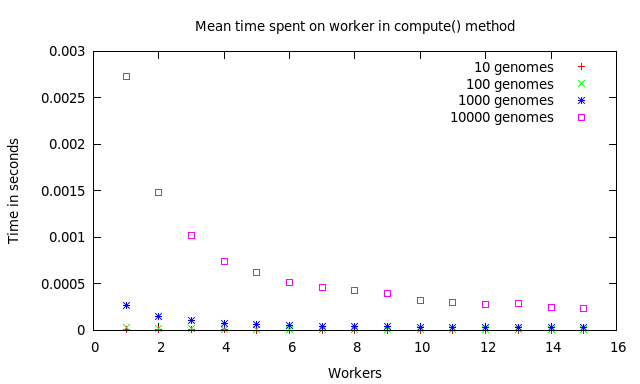
\includegraphics[width=100mm]{nsgaii-workertime.png}
%   \caption{ZDT-3 mean execution times spent on the workers \texttt{compute} method}
%   \label{fig:nsgaii-workertime}
% \end{figure}
% 
% The bad worker speedups for small genome sizes don't explain the bad algorithm speedups for bigger genome sizes, as the worker speedups for big genome sizes scale almost linearly. Figure \ref{fig:nsgaii-tasktime} helps to find a better suited explanation. It shows the mean time for the execution of a single task without the time spent in the workers \texttt{compute} method.
% 
% \begin{figure}
%   \centering
%   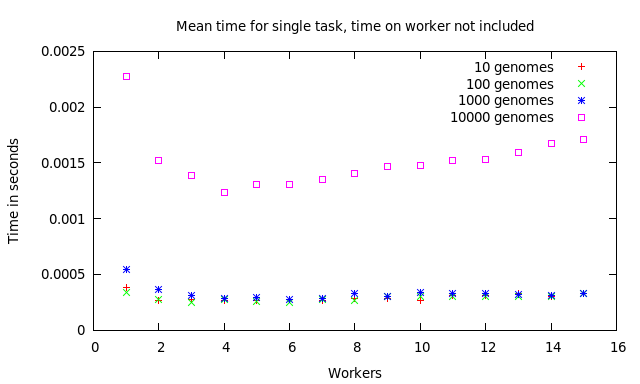
\includegraphics[width=100mm]{nsgaii-tasktime.png}
%   \caption{ZDT-3 mean execution times for a single task, without the time spent on the workers \texttt{compute} method}
%   \label{fig:nsgaii-tasktime}
% \end{figure}
% 
% One can see that the task time decreases for all benchmarks until two to four workers are used. Then it starts to increase. This behavior was not expected, rather it was expected that the task times keep decreasing as the number of workers increase because more tasks are executed in parallel.

The next step is to investigate the network performance. Calculations give a first hint to understand if the bad speedups can be explained with the saturation of the \unit[1]{Gb} network (a small ``b'' denotes bits, a big ``B'' denotes bytes, e.g., \unit[1]{Gb} = 1 gigabit, \unit[1]{GB} = 1 gigabyte). In each benchmark, 250 iterations on 100 individuals are performed, resulting in 25000 tasks. The tasks are send from the master to the workers and the workers return the results. The task data send from the master to the worker contains two individuals. Each individual consists of its genome, where each value in the genome is of type \texttt{double} (8 bytes). For a genome size of 10, this makes 2 (parents) $\times$ 10 (genomes) $\times$ 8 (bytes) $\times$ 25000 (tasks) = 4000000 bytes (\unit[4]{MB}) or \unit[32]{Mb} of data that needs to be transferred from the master to the workers during the benchmark. The size of the results send from the workers to the master is about the half, as it consists of an individual (the offspring) and its fitness (the fitness is composed of two \texttt{double} values). This fact allows to use the outgoing data amount as upper bound for the network usage: if the outgoing data rate doesn't exceed the network bandwidth. This will be true also for the incoming data. Table \ref{table:network} shows the results for all genome sizes together with the best algorithm execution times. One can see from the table that the benchmark data can be transferred on the \unit[1]{Gb} Ethernet network during the according fastest algorithm execution time.

\begin{table}
  \centering
  \begin{tabular}{r|r|r|r}
    genomes & data (Mb) & \parbox[t]{3cm}{theoretical\\transfer time (s)} & \parbox[t]{3cm}{fastest algorithm\\execution time (s)}\\ \hline
    10 & 32 & 0.032 & 7.072 \\
    100 & 320 & 0.32 & 7.031 \\
    1000 & 3200 & 3.2 & 8.910 \\
    10000 & 32000 & 32 & 55.475 \\
  \end{tabular}
  \caption{Amount of network data sent from master to workers, theoretical transfer time and fastest algorithm execution}
  \label{table:network}
\end{table}

% The calculations are supported by observations of the network performance using the iftop utility \cite{iftop}. This tool shows, among other useful statistics, the peak network bandwidth for a given interface. The outgoing peak bandwidth on the Ethernet port of the master machine for a genome size of 10000 was about 400Mb/s. This is clearly below the theoretical limit of 1Gb/s for the used 1Gb Ethernet network.

% But 400Mb/s are to slow to transmit 32Gb data in 55 seconds, so how is it possible that a benchmark for 10000 genomes terminates after 55s? The explanation can be found once more in the YARN container placement. The 400Mb/s is the data rate that is send through the Ethernet port to the cluster, but worker containers that run on the same machine as the master don't use this port for communication. Instead, they communicate through the local interface. iftop showed an additional combined data transfer rate of 400Mb/s on the local interface when workers were running on the same machine as the master. This gives an aggregated peak data rate of 600 - 700Mb/s for the outgoing traffic, which is fast enough to transmit 32Gb of data in less than 55s.
 
% In cases where no workers executed on the same machine as the master the peak data rates on the Ethernet port and the algorithm execution times were higher. The results of three different tests with a genome size of 10000 were: 445Mb/s peak and 80s execution time, 426Mb/s peak and 86s execution time and 447Mb/s peak and 80s execution time. In all cases the execution time is sufficient to transfer the data from the master through the Ethernet to the workers. The peak data rates were in all cases below maximum network speed of 1Gb/s.

Additional experiments were performed to improve the confidence in the calculations and to establish the true achievable data rate for the network, given different message sizes. The experiments measure the peak network bandwidth using a small Java program and iftop.\footnote{\url{http://www.ex-parrot.com/pdw/iftop/} last access: 08.12.2014} The Java program uses the same communication techniques as Biohadoop (Netty + Kryo) and performs repeated request/response cycles between a master and several workers. The exchanged messages consist of 20, 200, 2000 or 20000 \texttt{double} values, corresponding to two parent individuals in the according ZDT-3 benchmarks. The resulting peak bandwidth was \unit[134]{Mb/s} for 20, \unit[489]{Mb/s} for 200, \unit[901]{Mb/s} for 2000 and \unit[552]{Mb/s} for 20000 \texttt{double} values. The CPU on the master was the limiting factor for 20, 200 and 20000 \texttt{double} values. For 2000 \texttt{double} values, the network was saturated at \unit[901]{Mb/s} and, therefore, the limiting factor. No studies were performed to explain why the experiments delivered the best results with 2000 values as this lies out of the scope of this thesis.

One phenomena regarding the network bandwidth needs further investigation. The above measurements show a peak data rate of \unit[552]{Mb/s} for the case of 20000 \texttt{double} values. If this data rate is taken as a basis for the ZDT-3 benchmark with 10000 genomes, one can calculate that more than \unit[55]{s} are needed to exchange \unit[32]{Gb} of data over the network between the master and its workers (\unit[32000]{Mb} / \unit[552]{Mb/s} = \unit[57.97]{s}). The explanation can be found once more in the YARN container placement. The \unit[552]{Mb/s} peak bandwidth is the data rate that is send through the Ethernet port to the cluster, but worker containers that run on the same machine as the master don't use this port for communication. Instead, they communicate through the local interface. iftop showed an additional combined data transfer rate of \unit[400]{Mb/s} (send and receive data rates are added) on the local interface when workers were running on the same machine as the master. This gives an aggregated peak data rate of \unit[700]{Mb/s} to \unit[800]{Mb/s} for the outgoing traffic, which is fast enough to transmit \unit[32]{Gb} of data in less than \unit[55]{s}. The execution times were higher in cases where no workers executed on the same machine as the master.

The calculations and additional experiments show that the network is fast enough to transfer the ZDT-3 benchmark data. The reason for the bad ZDT-3 speedups lie elsewhere.

This leads to the assumption that the benchmarks are CPU bound which was confirmed through observations of the CPU usage of the master. In the case of 10 and 100 genomes the CPU limit was reached by the master with two workers, for 1000 and 10000 genomes the limit was reached with four workers.

The high CPU utilization is caused by two effects: the first one is the object serialization/deserialization overhead that ranges between \unit[30]{\%} to \unit[40]{\%} for genome sizes of 10 and goes up to \unit[60]{\%} to \unit[70]{\%} for a genome size of 10000. Small genome sizes mean a high rate of both exchanged messages and serializations/deserializations. Large genome sizes reduce the rate of exchanged messages but increase the amount of work for a single serialization/deserialization.

The second effect is a direct consequence of computationally small worker tasks like in the case of 10 to 100 genomes: the master performs (beside the communication aspects) the algorithms for ranking and crowding distance. The workers return their results fast as the computation is not intense. Therefore, the master has to compute the ranking and crowding distance at short intervals. This results in a CPU utilization of about \unit[25]{\%} to \unit[30]{\%} only for this computations.

In conclusion, the ZDT-3 benchmarks are CPU bound by the master due to the small computational effort on the workers and the resulting fast exchange of many small messages. Increased genome sizes provide better speedup results, but are again limited by the CPU of the master, as they have higher demands for object serialization/deserialization. The performance of the \unit[1]{Gb} network and the available memory are sufficient to not slow down the ZDT-3 benchmarks.

\subsection{Tiled Matrix Multiplication}
The optimization goal of this benchmark was to find optimal tile sizes such that a matrix multiplication performs as fast as possible. The theoretical speedups for TMM promise better results (see table \ref{table:theoretical_speedup}) as matrix multiplications are compute intense and clearly dominate the algorithm execution time. Figure \ref{fig:tiledmul_250_100_128x128} and \ref{fig:tiledmul_250_100_256x256} show the execution times. One can see that the execution times decrease with the number of workers. This scales until 12 workers, after which the execution times remain constant or even increase slightly. The reason for this is that the cluster offers 12 CPU cores in total. When all cores are fully utilized, which happens with 12 workers, additional workers have to share CPU resources. This negatively impacts the execution times. So, TMM is CPU bound by the workers.

\begin{figure}
  \centering
  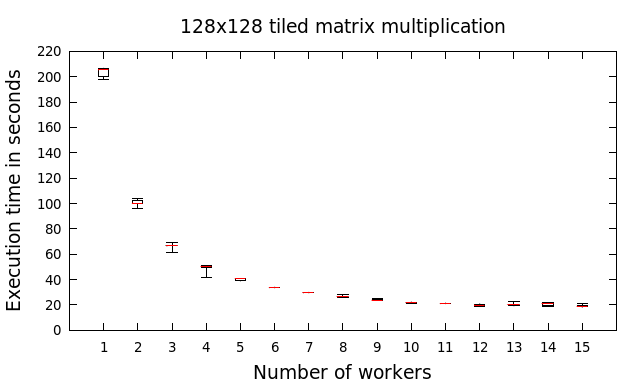
\includegraphics[width=100mm,natwidth=640,natheight=384]{tiledmul_250_100_128x128.png}
  \caption[TMM execution times for a matrix size of 128$\times$128]{TMM execution times for a matrix size of 128$\times$128}
  \label{fig:tiledmul_250_100_128x128}
\end{figure}
\begin{figure}
  \centering
  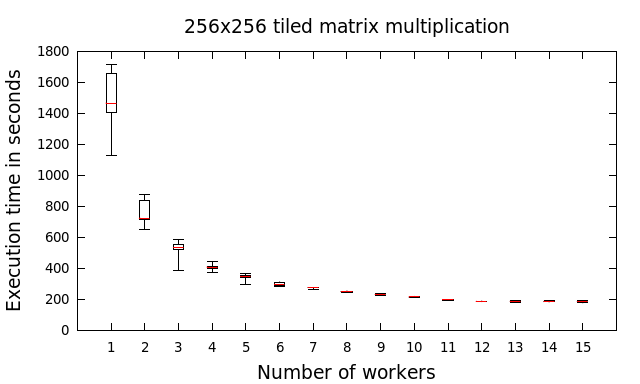
\includegraphics[width=100mm,natwidth=640,natheight=384]{tiledmul_250_100_256x256.png}
  \caption[TMM execution times for a matrix size of 256$\times$256]{TMM execution times for a matrix size of 256$\times$256}
  \label{fig:tiledmul_250_100_256x256}
\end{figure}

% The master is not as strongly demanded as in the ZDT-3 benchmarks, because the worker execution times are higher which results in less CPU stress on the master for object serialization/deserialization. Also, the master doesn't have to compute the ranking and crowding distance. 

An additional advantage of TMM benchmarks over the ZDT-3 benchmarks is the small amount of data that needs to be transmitted. Like in the ZDT-3 benchmarks, each task data consists of two parents that are sent from the master to the worker, the result is an offspring with its fitness value. In contrast to ZDT-3 --- where an individual consists of a number of \texttt{double} values according to its genome size --- a TMM individual consists of the tile sizes for the $i$, $j$ and $k$ loop. Each of them is a single \texttt{integer} with 4 bytes. The total amount of data that needs to be transmitted from the master to the workers is therefore $2 \times 3 \times 4 \times 25000 = 600000$ bytes or \unit[4.8]{Mb}. Together with the computationally intense tasks of matrix multiplication on the workers (leading to lower network usage) and the absence of time consuming ranking and crowding distance algorithms on the master, this provides speedups of up to 10.507 for 128$\times$128 matrices and 7.961 for 256$\times$256 matrices.

The reason for the better performance of the 128$\times$128 benchmark over the 256$\times$256 benchmark is unknown. A possible explanation is that the tile sizes are taken from a bigger range (256 instead of 128) which makes it more likely that bad tile sizes are chosen. This is, however, pure speculation.

% The results show less scattering in contrast to ZDT-3. This is due to the fact, that the matrix multiplications dominate the execution times. The location of the YARN containers and the time needed for the communication between the master and its workers have therefore a smaller impact on the execution times. Only the five benchmarks for \ref{fig:tiledmul_250_100_256x256} with one worker shows an elevated amount of scattering. The reason is unknown, as the master and the worker were located on different machines in all benchmarks with this settings. 

\subsection{Speedups}
Figure \ref{fig:speedup} depicts the speedups for all test problems with respect to increasing worker sizes. The ZDT-3 benchmarks show poor results. This is not surprising as the maximum theoretical speedups of this problem are small (see table \ref{table:theoretical_speedup}) and the communication overhead is bigger compared to TMM. The only unexpected outcome was that the benchmarks scale very bad with a maximum speedup of 2.498 for 1000 genomes. The reason is that the ZDT-3 benchmarks are CPU bound by the master, as the investigations in section \ref{chap:evaluation:result:zdt3} suggest.

TMM demonstrate better results, the maximum speedup was 10.507 for a matrix size of 128$\times$128. In this case, the speedup grows near linear or even slightly better than linear with the number of workers. That a speedup is better than linear is usually suspicious but can be explained by the fact that each benchmark was repeated five times and the average times of this five executions were taken to compute the speedups. Five executions seem to be too small for getting smooth results, especially when taking into account that the YARN container placement has big influences on the execution times.

The speedups for the 128$\times$128 TMM increase until a worker size of 12 is reached. At this point, no more improvements are achieved. The reason for this is the limited number of CPUs in the cluster.

The speedup for the 256$\times$256 TMM benchmark is worse compared to the 128$\times$128 TMM, although it also grows nearly linear until 12 workers.

\begin{figure}
  \centering
  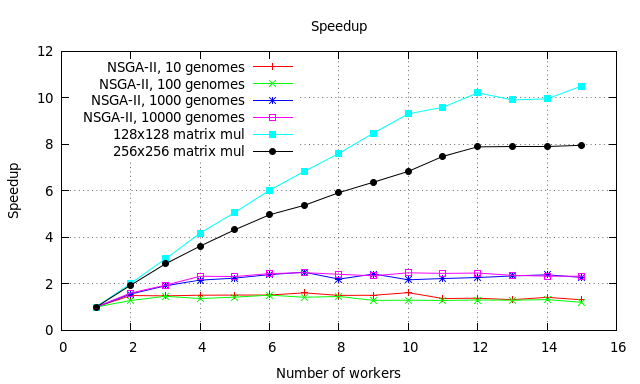
\includegraphics[width=130mm,natwidth=640,natheight=384]{speedup.png}
  \caption[Speedups for ZDT-3 and TMMs]{Speedups for ZDT-3 and TMMs}
  \label{fig:speedup}
\end{figure}

% 
% 
% Each physical machine in the cluster provides two cores, the master reaches its theoretical limit when it uses 200\% of the CPU resources, which means that both CPU are fully utilized by the master. The practical CPU limit is at about 150\%, because other processes run at the same time on the same machine. This limit is further reduced if worker containers are executed at the same time on the same machine. 
% 
% As each physical machine in the cluster provides two cores, the master reaches its theoretical limit when it uses 200\% of the CPU resources, which means that both CPU are fully utilized by the master. The practical CPU limit is at about 150\%, because other processes run at the same time on the same machine. This limit is further reduced if worker containers are executed at the same time on the same machine. 


% The ZDT-3 benchmarks show that the speedup does not scale well with the number of workers. The reason for this is that the time spent by the worker on offspring creation and fitness evaluation is only a small fraction of the time it takes to complete a task. For a genome size of 10 and one worker, this fraction is for example 2.124\% and reduces to 0.596\% for 15 workers. For a genome size of 100 the fraction ranges from 8.765\% for one worker to 1.138\% for 15 worker. For a genome size of 1000 it ranges from 33.100\% to 7.044\% and for a genome size of 10000 it ranges from 54.556\% to 11.789\%. So the ZDT-3 benchmark is clearly bound by the communication between the master and its workers. This explains also the overall poor scaling when workers are  added.
% 
% The execution time results for ZDT-3 are shown in figure \ref{fig:nsga_250_100_10}, \ref{fig:nsga_250_100_100}, \ref{fig:nsga_250_100_1000} and \ref{fig:nsga_250_100_10000}. One thing to notice is that the benchmark results for given settings are distributed in a broad range, e.g. they range from 9.637s to 14.164s for ZDT-3 with a genome size of 100 and one worker (see figure \ref{fig:nsga_250_100_100}).
% 
% % \begin{figure}
% %   \centering
% %   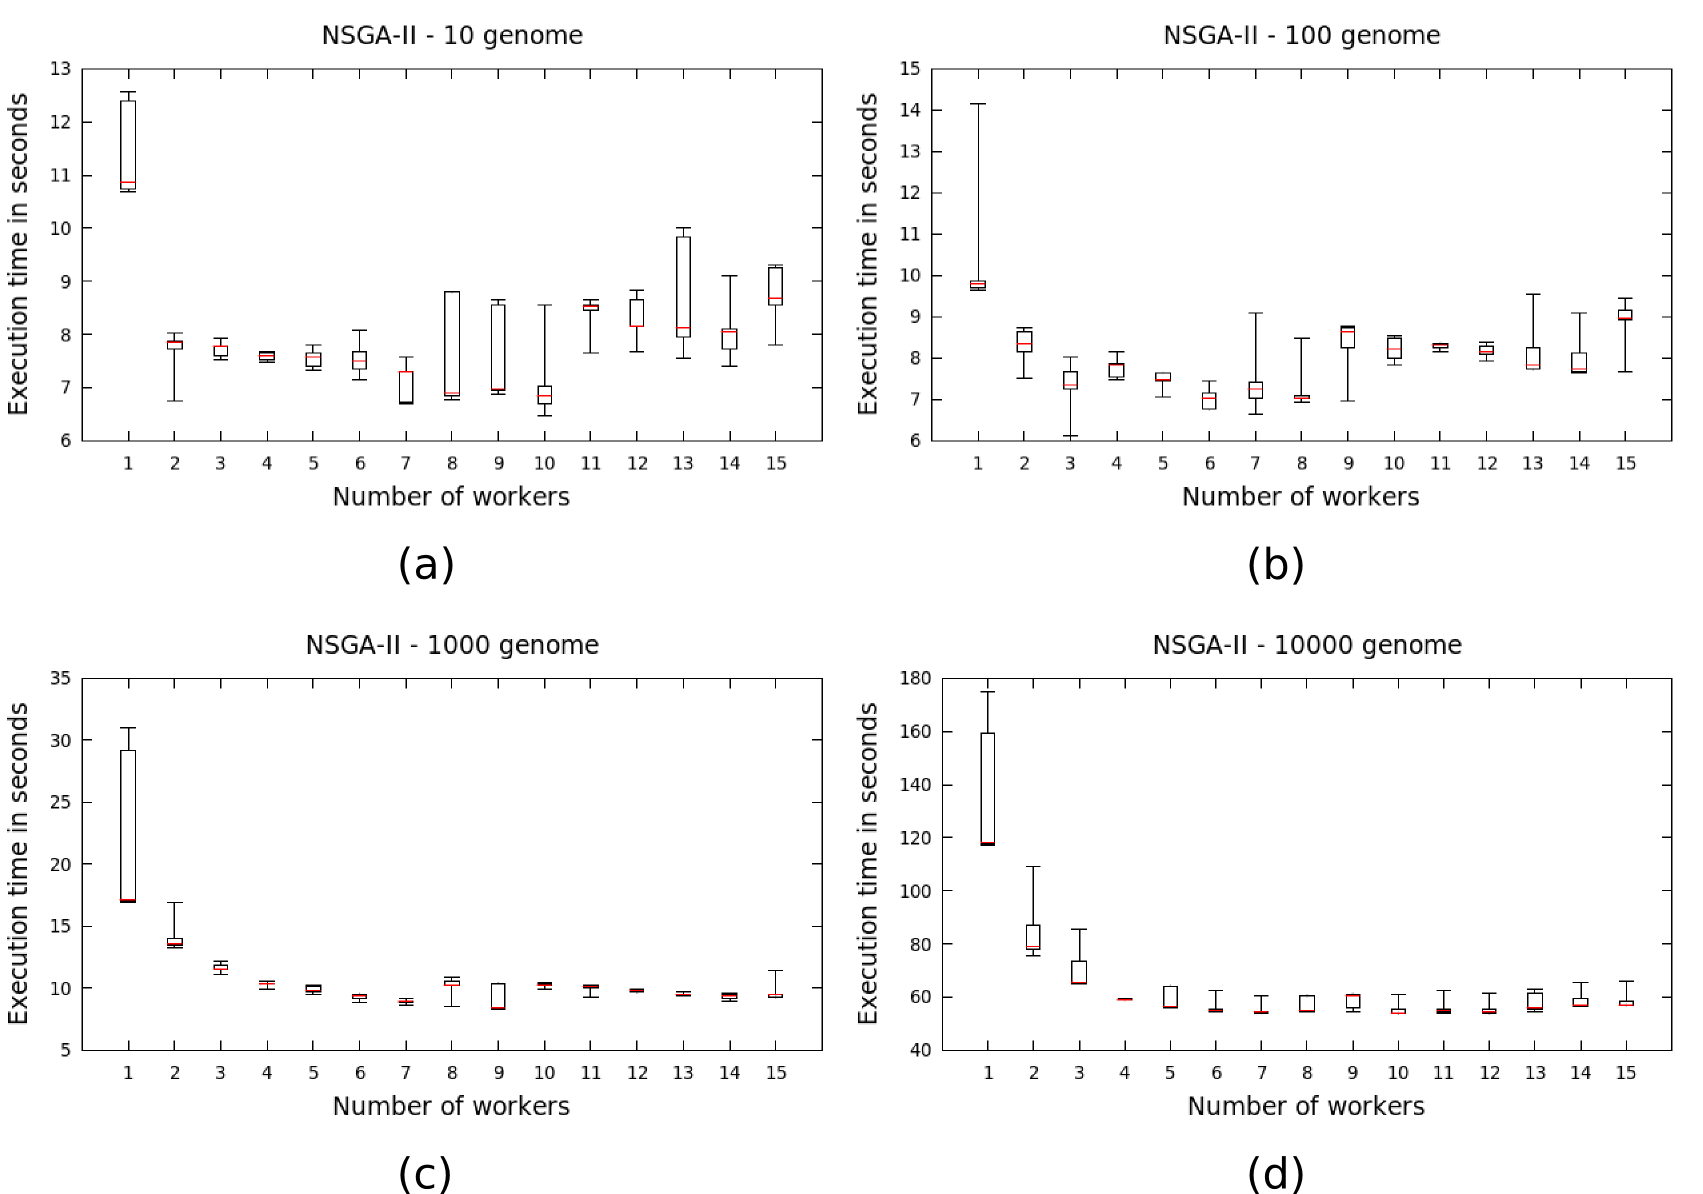
\includegraphics[width=130mm]{nsgaii_250_100.png}
% %   \caption{ZDT-3 execution times. All benchmarks were performed with 250 iterations and a population size of 100. (a) genome size=10, (b) genome size=100, (c) genome size=1000, (d) genome size=10000}
% %   \label{fig:nsga_250_100}
% % \end{figure}
% 
% 
% 
% The reason for this is the location of the YARN containers in the cluster while a benchmark runs. Figure \ref{fig:nsga_250_100_100} is used as example: for the benchmark with one worker, 4 out of 5 benchmarks executed with both the master and worker container running on the same machine, resulting in better performance. A worker that is located on the same machine as the master can communicate to the master without using a physical network, which reduces the communication time. During the fifth benchmark, the master and worker were executed on different containers. The 4 benchmarks with master and worker on the same machine took 9,761s on average, the benchmark where master and worker were located on different machines took 14.164s to execute.
% 
% The same explanation applies to the other benchmarks with 1 to 6 workers in figure \ref{fig:nsga_250_100_10} to \ref{fig:nsga_250_100_10000}, except for the benchmark for one worker in figure \ref{fig:nsga_250_100_10}. This deviation is not due of container placement, the scattered results are the result of other factors that couldn't be established.
% 
% The container placement is done automatically by YARN and can not be influenced, without modifying the YARN environment - which was not done for this thesis. The placement can have advantages like in the example above, but can also negatively impact the performance.
% 
% As an example, look at the benchmark for 8 workers in figure \ref{fig:nsga_250_100_10}. For two benchmarks, YARN placed the master and two worker containers on the same machine. As each machine has only two cores, this worsens the execution time results. The master container has to share its CPU resources with two other containers, that have already a high resource demand. This slows the master down and with it the whole application. The numbers for this example are 6.842s (on average) for the benchmarks where the master had to share its machine with only one worker. In the case the master were placed together with two other containers on the same machine the execution time was on average 8.799s.
% 
% The more the cluster is utilized, the more it is likely that more than two containers execute on the same machine. This can be particularly seen in figures \ref{fig:nsga_250_100_10} and \ref{fig:nsga_250_100_100} for the benchmarks with six and more workers.
% 
% Figure \ref{fig:nsga_250_100_1000} and \ref{fig:nsga_250_100_10000} show a similar but less pronounced behavior for more than six workers, as they are less communication bound than the previous examples. Both figures show a high dependency on the container placement for a small number of workers, e.g. for one worker.
% 
% Figure \ref{fig:nsga_250_100_10} shows that more than two workers have no significant impact on the execution time for a genome size of 10. The execution time remains almost the same when workers are added. The reason for this is the bad work time to task time ratio mentioned above. Figure \ref{fig:nsga_250_100_100} shows advantages for up to 9 workers for a genome size of 100 - if the container placement comes in favor. More workers increase the execution time. Figure \ref{fig:nsga_250_100_1000} shows also advantages for up to 9 workers for a genome size of 1000. The scattering is reduced in most of the figures benchmark, compared to the previous benchmarks. Figure \ref{fig:nsga_250_100_10000} shows the results for a genome size of 10000. The best results are obtained between 6 to 12 workers, more workers increase the execution time. The speedup properties for this benchmark are better compared to the previous ones, as the work time to task time ratio is way better.

% The theoretical speedups for TMM show better results (see table \ref{table:theoretical_speedup}), as matrix multiplications are compute intense and clearly dominate the algorithm execution time. Figure \ref{fig:tiledmul_250_100_128x128} and \ref{fig:tiledmul_250_100_256x256} shows the execution times for TMM test problem. The execution times for a matrix size of 128x128 are given in figure \ref{fig:tiledmul_250_100_128x128}. One can see that the execution time decreases with the number of workers. This scales until 12 workers, after which the execution time remains the same or slightly increases. The reason for this is, that the cluster offers 12 CPU cores in total. When all cores are fully utilized, which happens with 12 workers, additional workers have to share CPU cores. This negatively impacts the execution times. The same observations are true for figure \ref{fig:tiledmul_250_100_256x256}.
% 
% The results show less scattering in contrast to ZDT-3. This is due to the fact, that the matrix multiplications dominate the execution times. The location of the YARN containers and the time needed for the communication between the master and its workers have therefore a smaller impact on the execution times. Only the five benchmarks for \ref{fig:tiledmul_250_100_256x256} with one worker shows an elevated amount of scattering. The reason is unknown, as the master and the worker were located on different machines in all benchmarks with this settings. 
% 
% \begin{figure}
%   \centering
%   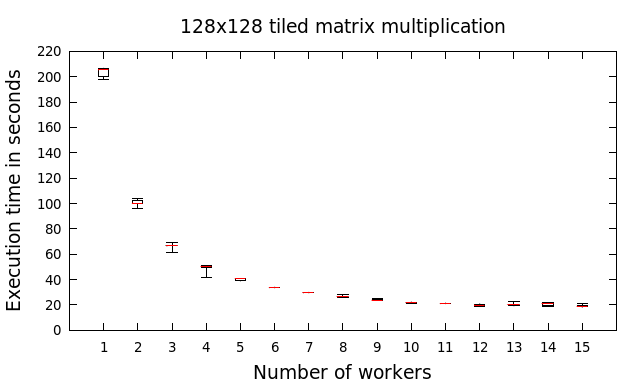
\includegraphics[width=100mm]{tiledmul_250_100_128x128.png}
%   \caption{TMM execution times. All benchmarks were performed with 250 iterations and a population size of 100. (a) matrix size=128x128, (b) matrix size=256x256}
%   \label{fig:tiledmul_250_100_128x128}
% \end{figure}
% \begin{figure}
%   \centering
%   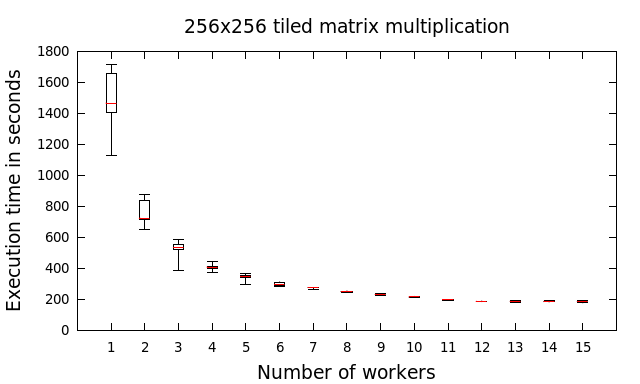
\includegraphics[width=100mm]{tiledmul_250_100_256x256.png}
%   \caption{TMM execution times. All benchmarks were performed with 250 iterations and a population size of 100. (a) matrix size=128x128, (b) matrix size=256x256}
%   \label{fig:tiledmul_250_100_256x256}
% \end{figure}
% 
% Figure \ref{fig:speedup} shows the speedups for all test problems with respect to increasing worker sizes. TMM shows good results. In the case of 128x128 TMM, the speedup grows near linear or even slightly better with the number of workers. That a speedup is better than linear was not expected but can be explained by the fact that each benchmark was repeated 5 five times, which seems to be to small to get smooth results. After 6 workers, the 128x128 benchmark shows good speedups until a worker size of 12 is reached. At this point, no more improvements are achieved, the reason for this is the number of CPUs in the cluster. The speedup for the 256x256 TMM benchmark is worse compared to the 128x128 TMM, although it grows nearly linear until 12 workers.
% 
% The speedups for the ZDT-3 benchmarks are not so good. Specially small genome sizes deliver poor results with speedups of less than 2 for genome sizes of 10 and 100, no matter how many workers are used. Increasing the genome size provides better results, using 1000 genomes provides a speedup of 2.498 using 7 workers. A genome size of 10000 provides a maximum speedup of 2.479 using 8 workers. Overall, the ZDT-3 benchmarks show only small improvements when workers are added, increasing the number of workers beyond 8 to 10 doesn't provide any benefit. This is not surprising as the maximum theoretical speedups of this problems are small (see table \ref{table:theoretical_speedup}) and the communication overhead is bigger compared to TMM.
% 
% \begin{figure}
%   \centering
%   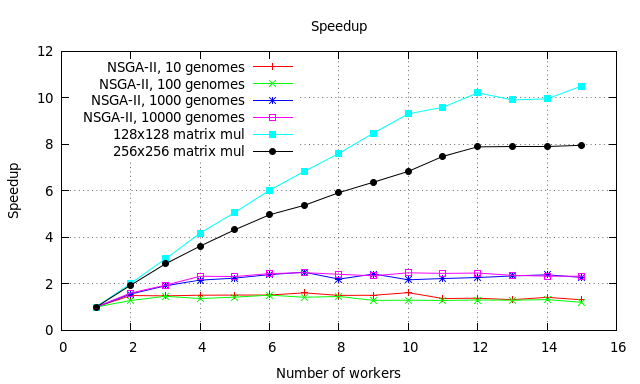
\includegraphics[width=130mm]{speedup.png}
%   \caption{Speedup for ZDT-3 and TMM}
%   \label{fig:speedup}
% \end{figure}
% 
% Another observation was, that the number of worker containers running on the same machine as the master could affected the execution times negatively.
% \chapter{Conclusions}
\label{chap:conclusions}
This thesis presented Biohadoop, a new framework to build bio-inspired optimization techniques executable on Apache Hadoop. Two different GAs were implemented on top of Biohadoop. Their performance was evaluated on a Hadoop cluster with 6 dual-core computers that were connected to a \unit[1]{Gb} Ethernet network.

The results show that algorithms implemented with Biohadoop have the potential to scale efficiently if the parallel part of the problem dominates the whole execution time. An example of such a problem is the tiled matrix multiplication (TMM). It provided speedups of up to 10 when compared to the execution with less resources (one worker). ZDT-3 as the other benchmark exposed a behavior that lead to poor speedups of about 2. The problem with this benchmark was that the parallel running parts were very short in terms of computational time. The sequential time and communication overhead dominated the whole runtime.

The execution time comparison with standalone, sequential implementations demonstrated further advantages of Biohadoop. TMM provided in this case speedups of about 8. In contrast, the performance of ZDT-3 was worse to the point that the parallel execution took longer than the sequential version.

In conclusion, Biohadoop demonstrated to be a useful framework for the implementation of bio-inspired optimization techniques on Hadoop. It provides a powerful non-blocking API that simplifies the design of distributed applications. Hadoop as solid and well tested basis provides the necessary cluster management and reliable application execution. Further, the evaluation results show that algorithms suited to parallelization and implemented with Biohadoop achieve good speedups. Those properties make Biohadoop a good match for the implementation and execution of parallelized bio-inspired optimization techniques on Hadoop.
% 
% 
% The evaluation results show that algorithms suited to parallelization can achieve good speedups when implemented with Biohadoop. Using Hadoop for cluster management and reliable application execution, 
% 
% 
% 
% In conclusion, the evaluation results show that Biohadoop is a useful framework for the implementation of bio-inspired optimization techniques. It provides a simple and powerful non-blocking API for distributed computations. It was demonstrated that algorithms suited to parallelization can achieve good speedups. This is accomplished by 
% 
%  and . Biohadoop relies on Hadoop for cluster management and reliable execution of parallelized algorithms
% Biohadoop uses Hadoop for reliable execution of parallelized algorithms on a cluster. It was demonstrated that algorithms suited to parallelization can achieve good speedups. This properties make Biohadoop a good match for the implementation and execution of parallelized bio-inspired optimization techniques on Hadoop.
% 
% 
% Given that an algorithm is well suited for parallelization, Biohadoop offers an easy way for its implementation. The evaluation demonstrated also that such parallelized algorithms are able to perform very well on Hadoop.
% 
% In conclusion, the evaluation results show that Biohadoop is a useful framework for the implementation of bio-inspired optimization techniques. The underlying Hadoop system provides with HDFS and YANR a solid basis for the execution. Biohadoop provides a simple but powerful non-blocking API for distributed computations
% 
% 
% 
% In conclusion, the evaluation results show that Biohadoop is a useful framework for the implementation of bio-inspired optimization techniques on Hadoop. It provides a simple but powerful non-blocking API for distributed computations that otherwise needs to be implemented manually. Hadoop as basis layer simplifies cluster usage and reliable application execution.
% END: content -------------------------------------------------------

%%\input{literaturverzeichnis}
%%\printglossary
% BEGIN: appendix ----------------------------------------------------
\appendix
\addappheadtotoc

\chapter{}

\section{How to Run Biohadoop}
\label{chap:usage:run}
Although, the main purpose of Biohadoop is to be run in a Hadoop environment, it can also be run in a local environment. This is for example useful when new algorithms are developed. In this case, the whole process of compilation, deployment to a Hadoop environment and testing can be abbreviated.

To run Biohadoop, three components must be available (four if Biohadoop is started in a Hadoop environment):

\begin{itemize}
  \item An installation of Java in version 1.7 or higher. From here on it is assumed, that Java is installed and configured and that the \texttt{JAVA\_HOME} environment variable points to this installation.
  \item All necessary libraries must be present and accessible in one or several folders.
  \item A valid configuration file must be present and accessible.
  \item The fourth component is only necessary when running Biohadoop in a Hadoop environment. This component is Hadoop itself, which must be available in a version $\geq 2$.
\end{itemize}

If those three components are provided (four for running on Hadoop), Biohadoop can be started. In a local environment, this is done by setting the right class paths when launching the program. In a Hadoop environment, the configuration option \texttt{includePaths} must be set, to include the necessary files (see section \ref{chap:impl:configuration} on more information about how to configure Biohadoop). Those paths have to point to valid locations of an accessible HDFS file system.

Biohadoop was developed using Maven.\footnote{\url{http://maven.apache.org/} last access: 11.09.2014} Therefore, it is rather easy to get all the needed libraries, since they are declared as dependencies. The source code for Biohadoop can be found on GitHub: \url{https://github.com/gappc/biohadoop/}. By invoking the following command on the projects root folder, all dependencies are accumulated and put to the sub folder \texttt{target/dependency}:

\begin{lstlisting}[language=bash]
mvn dependency:copy-dependencies
\end{lstlisting}

From there, they can be directly referenced through Javas \texttt{classpath} option when running in a local environment. When running in a Hadoop environment, the libraries need to be copied to an accessible HDFS file system, and this location must be present in the \texttt{includePaths} configuration option mentioned above.

% For a quick tutorial on how to compile and run Biohadoop from the sources, please refer to appendix \ref{chap:appendix:biohadoop-quickstart}. 
To use Biohadoop in a Hadoop environment, such an environment must be present. It can be a difficult task to configure such a Hadoop environment, therefore, in appendix \ref{chap:appendix:biohadoop-docker} a simple method can be found, to use a pre-build Hadoop environment. The only dependency which this environment has is Docker.\footnote{\url{https://www.docker.com/} last access: 11.09.2014} Docker is a simple and lightweight runtime for virtual containers available on all major operating systems.

\subsection{Local Environment}
\label{chap:usage:local}
To start Biohadoop in a local environment, the class paths need to be set to include the necessary libraries. The necessary libraries can be obtained by invoking the Maven command, outlined above. As an additional parameter, the \texttt{-Dlocal} option must be provided to Java. This is the only way to tell Biohadoop that it is launched in a local environment. If this parameter is missing Biohadoop can't connect to Hadoop.

Lets assume, that all of the necessary libraries can be found at the location \path{/home/user/biohadoop/libs}, and the configuration file can be found at \path{/home/user/biohadoop/configs/simple-config-json}. Then, Biohadoop can be started in local mode by running the following command:
  
\begin{lstlisting}[language=bash]
java -Dlocal -cp /home/user/biohadoop/libs/* at.ac.uibk.dps.biohadoop.hadoop.BiohadoopApplicationMaster /home/user/biohadoop/configs/simple-config-json
\end{lstlisting}

A little bit hidden in the command we find the main class that starts Biohadoop, \texttt{at.ac.uibk.dps.biohadoop.hadoop.BiohadoopApplicationMaster}. This class takes care of starting the configured algorithms, endpoints and workers. After all of the algorithms have terminated, either because they have finished their computation or because of errors, Biohadoop shuts down.

When running Biohadoop in the local environment, all workers are started as threads in the same JVM as Biohadoop (in contrast to a Hadoop environment, where the workers are started in separate JVMs on perhaps different machines). This leads to the fact, that the workers have full access to all (static) objects of Biohadoop. But when those workers are started in a Hadoop environment, this access is not given anymore. So, one has to take care to rely only on the objects and properties that are provided to the used methods.

\subsection{Hadoop Environment}
\label{chap:usage:hadoop}
To start Biohadoop in a Hadoop environment (for example in the one provided in appendix \ref{chap:appendix:biohadoop-docker}), all needed libraries and configuration files must be present in the HDFS file system. In addition, Biohadoops jar file, i.e., the compiled library, must be accessible through the local file system, as it is started directly by Hadoop. The location of the libraries and configuration files in the HDFS file system must be configured in the configuration file that is provided to Biohadoop on startup.

Lets assume, that all of the necessary libraries can be found at the HDFS location \path{/biohadoop/libs}, the configuration file can be found at the HDFS location \path{/biohadoop/configs/simple-config-json} and that those paths are part of the configuration file that is provided to Biohadoop at startup. Furthermore, Biohadoops jar file can be found at \path{/home/user/biohadoop/biohadoop.jar}. Then, Biohadoop can be started in Hadoop mode by running the following command:

\begin{lstlisting}[language=bash]
yarn jar /home/user/biohadoop/biohadoop.jar at.ac.uibk.dps.biohadoop.hadoop.BiohadoopClient /biohadoop/configs/simple-config-json
\end{lstlisting}

As one can see, now the command \texttt{yarn} is used to launch Biohadoop. This command takes care of setting all the needed Hadoop environment variables, after which it starts the provided main class. The \texttt{yarn} command is part of Hadoop since version 2, and should be available if Hadoop is configured correctly.

In contrast to running Biohadoop in local mode, we have now a different main class that is launched. This is due to the fact, that Yarn needs a startup class, from where it loads the main program. By looking at the source code of \texttt{at.ac.uibk.dps.biohadoop.hadoop.BiohadoopClient}, one will notice that it starts the \texttt{BiohadoopApplicationMaster} behind the curtains (\texttt{BiohadoopApplicationMaster} is the class that is directly started in local mode).

When running Biohadoop in a Hadoop environment, all workers are started in their own containers, which are under the control of Hadoop. The result is, that the workers can not access the (static) objects of Biohadoop, if one wants to access some properties of Biohadoop, this must be done through the provided communication facilities of Biohadoop. It is nevertheless possible to implement some different communication facilities, if this is needed.

% \section{JSON Schema for Biohadoops configuration file}
% \lstinputlisting[caption=JSON Schema \cite{json-schema} for the Biohadoop configuration file,label=lst:json-schema]{../listings/appendix-configuration-schema.lst}

% \section{Example algorithm: Sum}
% \lstinputlisting[caption=Source code for the example \texttt{Sum} algorithm\, elaborated in chapter \ref{chap:usage},label=lst:appendix-sum-full]{../listings/appendix-sum-full.lst}
% 
% \section{Example algorithm: Sum - AsyncComputable}
% \lstinputlisting[caption=Source code for the \texttt{AsyncSumComputation} part of the \texttt{Sum} algorithm\, elaborated in chapter \ref{chap:usage},label=lst:appendix-sum-async]{../listings/appendix-sum-async.lst}

% \section{Biohadoop quickstart}
% \label{chap:appendix:biohadoop-quickstart}
% The quickstart uses the pre-configured Hadoop environment, that can be found in appendix \ref{chap:appendix:biohadoop-docker}. This environment is installed during the following steps. In addition, some example algorithms are installed, that can be found at \cite{biohadoop-algorithms}. 
% 
% The requirements for this quickstart are Docker $\geq 1.0$, Maven with MVN\_HOME set to the correct path and an installed gnome-terminal (provided by default in Ubuntu). The quickstart takes usage of some scripts, all of them are provided by the used sources.
% 
% \subsection{Build and start the Hadoop environment}
% The first step is to build and start a Hadoop environment with one master and two slave nodes. The master node is started inside a red gnome-terminal window, at the end it prints the password for the root user:
% 
% \begin{lstlisting}[language=bash]
% git clone https://github.com/gappc/docker-biohadoop.git
% sudo docker build -t="docker-biohadoop" ./docker-biohadoop
% chmod +x ./docker-biohadoop/scripts/*.sh
% ./docker-biohadoop/scripts/docker-run-hadoop.sh 2
% \end{lstlisting}
% 
% \subsection{Build Biohadoop and copy it to the Hadoop environment}
% The second step is to build and copy Biohadoop to the Hadoop environment:
% 
% \begin{lstlisting}[language=bash]
% git clone https://github.com/gappc/biohadoop.git
% chmod +x ./biohadoop/scripts/*.sh
% ./biohadoop/scripts/copy-files.sh
% \end{lstlisting}
% 
% \subsection{Build example algorithms and copy them to the Hadoop environment}
% The third step is to build and copy the example algorithms to the Hadoop environment:
% 
% \begin{lstlisting}[language=bash]
% git clone https://github.com/gappc/biohadoop-algorithms.git
% chmod +x ./biohadoop-algorithms/scripts/*.sh
% ./biohadoop-algorithms/scripts/copy-algorithms.sh
% \end{lstlisting}
% 
% \subsection{Run Biohadoop in the Hadoop environment}
% To run the Echo example in Hadoop , the following command must be issued in the red terminal - if there is no red terminal, please check \cite{biohadoop-docker}. This example assumes that the jar \texttt{biohadoop-0.3.0-SNAPSHOT.jar} is used:
% 
% \begin{lstlisting}[language=bash]
% yarn jar /tmp/lib/biohadoop-0.3.0-SNAPSHOT.jar at.ac.uibk.dps.biohadoop.hadoop.BiohadoopClient /biohadoop/conf/biohadoop-echo.json
% \end{lstlisting}
% 
% Other examples of Biohadoop programs can be found at \cite{biohadoop-algorithms}. You can use them to try out Biohadoop and as a template for your own experiments. Good luck and have fun :)

\section{Pre-build Hadoop Environment using Docker}
\label{chap:appendix:biohadoop-docker}
This section provides a method to run a pre-configured Hadoop environment using Docker. Docker uses its so called Dockerfiles for its configuration. The solution presented here installs Apache Hadoop 2.5.0, Apache Oozie 4.0.1 and Apache ZooKeeper 3.4.6 as a cluster environment.

\subsection{Build the Hadoop Environment}
The following commands are used to clone the repository to the current local directory and to build the Docker image. Be aware that during the cloning process about 400MB of data is transferred. This is due to Oozie, which is delivered in a precompiled form.
\begin{lstlisting}[language=bash]
git clone https://github.com/gappc/docker-biohadoop.git
cd docker-biohadoop
sudo docker build -t="docker-biohadoop" .
\end{lstlisting}

The project \texttt{docker-biohadoop} provides two scripts, located in the scripts directory, that can be used to start and stop \texttt{docker-biohadoop} instances. Those scripts need to be executable:

\begin{lstlisting}[language=bash]
chmod +x scripts/*.sh
\end{lstlisting}

\subsection{Run Hadoop}
After that, we are able to start Hadoop instances by using the first script: \texttt{docker-run-hadoop.sh}. This script starts a number of Hadoop instances. It takes the number of slaves (nr-of-slaves) as argument. The script starts one Docker container as Hadoop master and additional nr-of-slaves Docker containers as Hadoop slaves. For example, one Hadoop master instance and two slaves are started by the following command:

\begin{lstlisting}[language=bash]
scripts/docker-run-hadoop.sh 2
\end{lstlisting}

Note that also the master is used for computational purposes. Therefor, Hadoop has 3 machines for computation with the settings above.

After invoking \texttt{docker-run-hadoop.sh}, a gnome-terminal is started for every Docker container. The master containers terminal has a red color, the slaves terminals are yellow. The master container starts the Hadoop environment, which may take some time (depending on the hardware and the number of slaves). After this initialization, the Hadoop cluster is ready for usage. Try to invoke the command \texttt{jps} on all running containers to look if Hadoop is running:

\begin{lstlisting}[language=bash]
jps
\end{lstlisting}

On the master node, it should output:
\begin{itemize}
  \item DataNode
  \item JobHistoryServer
  \item NodeManager
  \item NameNode
  \item QuorumPeerMain
  \item ResourceManager
  \item SecondaryNameNode
\end{itemize}

On the slave nodes it should output:
\begin{itemize}
  \item DataNode
  \item NodeManager
\end{itemize}

\subsection{Stopping Hadoop}
By using the following command, all running Docker containers are forcefully stopped and their interfaces are removed from the host. It is no problem to forcefully stop Docker containers, as they don't keep any state by default.
\begin{lstlisting}[language=bash]
scripts/docker-stop-all.sh
\end{lstlisting}

\subsection{SSH access}
The master node is accessible with user root, a password is generated on each startup and printed on the master terminal. Consider adding your SSH key to the Dockerfile if you are going to use \texttt{docker-biohadoop} often.

% \section{Biohadoop example workflow.xml}
% \begin{lstlisting}[label=lst:biooozie, language=XML]
% <workflow-app xmlns="uri:oozie:workflow:0.2" name="biohadoop-wf">
%     <start to="biohadoop-node"/>
%     <action name="biohadoop-node">
%         <biohadoop xmlns="uri:custom:biohadoop-action:0.1">
%             <name-node>hdfs://master:54310</name-node>
%             <config-file>/biohadoop/conf/biohadoop-algorithm-1.json</config-file>
%             <config-file>/biohadoop/conf/biohadoop-algorithm-2.json</config-file>
%         </biohadoop>
%         <ok to="end"/>
%         <error to="fail"/>
%     </action>
%     <kill name="fail">
%         <message>Biohadoop failed, error message[${wf:errorMessage(wf:lastErrorNode())}]</message>
%     </kill>
%     <end name="end"/>
% </workflow-app>
% \end{lstlisting}
% END: appendix ------------------------------------------------------




\listoffigures

\listoftables

\lstlistoflistings

% -+-+-+-+-+     .bib FILE MUST BE CALLED biblio.bib -+-+-+-+-+-+-+-
\bibliographystyle{unsrt}
\selectlanguage{english}
\bibliography{biblio}

\end{document}


